% $Header$
% MBDyn (C) is a multibody analysis code.
% http://www.mbdyn.org
%
% Copyright (C) 1996-2011
%
% Pierangelo Masarati  <masarati@aero.polimi.it>
%
% Dipartimento di Ingegneria Aerospaziale - Politecnico di Milano
% via La Masa, 34 - 20156 Milano, Italy
% http://www.aero.polimi.it
%
% Changing this copyright notice is forbidden.
%
% This program is free software; you can redistribute it and/or modify
% it under the terms of the GNU General Public License as published by
% the Free Software Foundation (version 2 of the License).
% 
%
% This program is distributed in the hope that it will be useful,
% but WITHOUT ANY WARRANTY; without even the implied warranty of
% MERCHANTABILITY or FITNESS FOR A PARTICULAR PURPOSE.  See the
% GNU General Public License for more details.
%
% You should have received a copy of the GNU General Public License
% along with this program; if not, write to the Free Software
% Foundation, Inc., 59 Temple Place, Suite 330, Boston, MA  02111-1307  USA
%
% Copyright (C) 2008
%
% Marco Morandini

\chapter{Elements}\label{sec:ELEMENTS}
The \kw{elements} section is enclosed in the cards:
%\begin{verbatim}
\begin{Verbatim}[commandchars=\\\{\}]
    \kw{begin} : \kw{elements} ;
        # ...
    \kw{end} : \kw{elements} ;
\end{Verbatim}
%\end{verbatim}
Every element card has the following format:
%\begin{verbatim}
\begin{Verbatim}[commandchars=\\\{\}]
    \bnt{card} ::= \bnt{elem_type} :
        \bnt{arglist}
        [ , \kw{output} , \{ \kw{yes} | \kw{no} \} ] 
        [ , \bnt{extra_arglist} ] ;
\end{Verbatim}
%\end{verbatim}
where \nt{elem\_type} is one of the following:
\begin{itemize}
\item structural elements:
\begin{itemize}
\item \kw{automatic structural}
\item \kw{beam}
\item \kw{body}
\item \kw{couple}
\item \kw{gravity}
\item \kw{joint}
\item \kw{joint regularization}
\item \kw{plate}
\end{itemize}

\item aerodynamic elements:
\begin{itemize}
\item \kw{aerodynamic beam2}
\item \kw{aerodynamic beam3}
\item \kw{aerodynamic body}
\item \kw{aeromodal}
\item \kw{aircraft instruments}
\item \kw{air properties}
\item \kw{induced velocity}
\end{itemize}

\item electric elements:
\begin{itemize}
\item \kw{electric}
\end{itemize}

\item hydraulic elements:
\begin{itemize}
\item \kw{hydraulic}
\end{itemize}

\item thermal elements:
\begin{itemize}
\item TODO \ldots
\end{itemize}

\item output elements:
\begin{itemize}
\item \kw{RTAI output}
\item \kw{stream output}
\item \kw{stream motion output}
\end{itemize}

\item generic elements:
\begin{itemize}
\item \kw{bind}
\item \kw{bulk}
\item \kw{force}
\item \kw{genel}
\item \kw{loadable}
\item \kw{user defined}
\end{itemize}

\item miscellaneous element cards
\end{itemize}


In case of elements that can be instantiated only once, like
the \kw{gravity} or the \kw{air properties} elements, the \nt{arglist}
does not contain any label; otherwise, a label is expected first, to allow 
for checks on duplicated elements, namely: 
%\begin{verbatim}
\begin{Verbatim}[commandchars=\\\{\}]
    \bnt{arglist} ::= \bnt{label} , \bnt{normal_arglist}
\end{Verbatim}
%\end{verbatim}
The data manager reads the element type and the label and checks for
duplication. If the element is not defined yet, the proper read function is
called, which parses the rest of the card and constructs the element.
The elements are read as follows.



% $Header$
% MBDyn (C) is a multibody analysis code.
% http://www.mbdyn.org
%
% Copyright (C) 1996-2010
%
% Pierangelo Masarati  <masarati@aero.polimi.it>
%
% Dipartimento di Ingegneria Aerospaziale - Politecnico di Milano
% via La Masa, 34 - 20156 Milano, Italy
% http://www.aero.polimi.it
%
% Changing this copyright notice is forbidden.
%
% This program is free software; you can redistribute it and/or modify
% it under the terms of the GNU General Public License as published by
% the Free Software Foundation (version 2 of the License).
% 
%
% This program is distributed in the hope that it will be useful,
% but WITHOUT ANY WARRANTY; without even the implied warranty of
% MERCHANTABILITY or FITNESS FOR A PARTICULAR PURPOSE.  See the
% GNU General Public License for more details.
%
% You should have received a copy of the GNU General Public License
% along with this program; if not, write to the Free Software
% Foundation, Inc., 59 Temple Place, Suite 330, Boston, MA  02111-1307  USA

\section{Aerodynamic Elements}
\label{sec:EL:AERO}


\subsection{Aerodynamic Body/Aerodynamic Beam2/3}
\label{sec:EL:AERO:BODY-BEAM23}
These elements share the description of the aerodynamics.
The former assumes the aerodynamic surface to be rigid,
and takes its configuration from a single node, while the latter
respectively relie on a two or three-node beam
and use the same interpolation functions of the beam to compute
the configuration at an arbitrary point.

The input format is:
%\begin{verbatim}
\begin{Verbatim}[commandchars=\\\{\}]
    \bnt{elem_type} ::= \{ \kw{aerodynamic body} | \kw{aerodynamic beam2} | \kw{aerodynamic beam3} \}

    \bnt{normal_arglist} ::= \bnt{connectivity} ,
        (\ty{Shape<1D>})          \bnt{surface_chord} ,
        (\ty{Shape<1D>})          \bnt{surface_aerodynamic_center} ,
        (\ty{Shape<1D>})          \bnt{surface_b_c_point} ,
        (\ty{Shape<1D>})          \bnt{surface_twist} ,
        [ \kw{tip loss} , (\ty{Shape<1D>}) \bnt{tip_loss} , ]
        \bnt{integration_points}
        [ , \kw{control} , (\ty{DriveCaller}) \bnt{control_drive} ] 
        [ , \bnt{airfoil_data} ]
        [ , \kw{unsteady} , \{ \kw{bielawa} \} ]
        [ , \kw{jacobian} , \{ \kw{yes} | \kw{no} | \bnt{bool} \} ]
        [ , \bnt{custom_output} ]

    \bnt{extra_arglist} ::= \{ \kw{std} | \kw{gauss} | \kw{node} \}
\end{Verbatim}
%\end{verbatim}
where
%\begin{verbatim}
\begin{Verbatim}[commandchars=\\\{\}]
    \bnt{connectivity} ::= \{ \bnt{body_conn} | \bnt{beam2_conn} | \bnt{beam3_conn} \}

    # \bnt{elem_type} ::= \kw{aerodynamic body}
    \bnt{body_conn} ::= \bnt{node_label}
        [ , [ \kw{user defined} ] \kw{induced velocity} , \bnt{induced_velocity_label} ] ,
        (\ty{Vec3})              <relative_surface_offset> , 
        (\ty{OrientationMatrix}) <relative_surface_orientation> ,
        (\ty{Scalar})            <surface_span>

    # \bnt{elem_type} ::= \kw{aerodynamic beam2}
    \bnt{beam2_conn} ::= \bnt{beam2_label}
        [ , [ \kw{user defined} ] \kw{induced velocity} , \bnt{induced_velocity_label} ] ,
        (\ty{Vec3})              \bnt{relative_surface_offset_1} ,
        (\ty{OrientationMatrix}) \bnt{relative_surface_orientation_1} ,
        (\ty{Vec3})              \bnt{relative_surface_offset_2} ,
        (\ty{OrientationMatrix}) \bnt{relative_surface_orientation_2} ,

    # \bnt{elem_type} ::= \kw{aerodynamic beam3}
    \bnt{beam3_conn} ::= \bnt{beam3_label} 
        [ , [ \kw{user defined} ] \kw{induced velocity} , \bnt{induced_velocity_label} ] ,
        (\ty{Vec3})              \bnt{relative_surface_offset_1} ,
        (\ty{OrientationMatrix}) \bnt{relative_surface_orientation_1} ,
        (\ty{Vec3})              \bnt{relative_surface_offset_2} ,
        (\ty{OrientationMatrix}) \bnt{relative_surface_orientation_2} ,
        (\ty{Vec3})              \bnt{relative_surface_offset_3} ,       
        (\ty{OrientationMatrix}) \bnt{relative_surface_orientation_3} ,

    \bnt{airfoil_data} ::=
        \{ \kw{naca 0012}
            | \kw{rae 9671}
            | [ \kw{theodorsen} , ] \kw{c81} , \bnt{c81_data} \}
\end{Verbatim}
%\end{verbatim}
and
%\begin{verbatim}
\begin{Verbatim}[commandchars=\\\{\}]
    \bnt{c81_data} ::=
        \{ \bnt{c81_label}
            | \kw{multiple} , \bnt{airfoil_number} ,
                \bnt{c81_label} , \bnt{end_point}
                [ , ... ]
            | \kw{interpolated} , \bnt{airfoil_number} ,
                \bnt{c81_label} , \bnt{position}
                [ , ... ] \}
\end{Verbatim}
%\end{verbatim}
The \nt{custom\_output} optional data consists in
%\begin{verbatim}
\begin{Verbatim}[commandchars=\\\{\}]
    \bnt{custom_output} ::= \kw{custom output} , 
        \bnt{custom_output_flag} [ , ... ]
\end{Verbatim}
%\end{verbatim}
The values of \nt{custom\_output\_flag}
are defined in Section~\ref{sec:CONTROLDATA:DEFAULTAERODYNAMICOUTPUT}.

Flags add up to form the custom output request.
Flags may not be repeated.
By default, only forces are output.
The custom output is only available in NetCDF format;
see Section~\ref{sec:NetCDF:Elem:Aerodynamic}.

The field \nt{induced\_velocity} indicates the label
of the \kw{induced velocity} element that this element is linked to.
This means that the element can get information about the
induced velocity and should supply information about the forces it generates.
If the keyword \kw{user defined induced velocity} is used,
then \nt{induced\_velocity} refers to a \kw{user defined} element.
Note: if the keyword \kw{induced velocity} is used
and no induced velocity element is found with the label \nt{induced velocity}
a \kw{user defined} element with that label is looked up.

An arbitrary relative orientation and offset is allowed for all elements with
respect to the nodes they are linked to. 
This means that the aerodynamic beam offsets refer to the position
of the beam's nodes, and have nothing to do with offsets related
to the structural beam element.

The \ty{Shape<1D>} entities are used to compute the physical chord,
aerodynamic center, velocity measurement point (the point where the
kinematic boundary conditions are evaluated) and twist as functions 
of the dimensionless abscissa along the span.

The optional \kw{tip loss} keyword allows to define an additional shape,
\nt{tip\_loss},
whose value is used to scale the value of the normal aerodynamic force.
By default, the scale factor is 1.
The \nt{tip\_loss} shape should have a value comprised between 0 and 1.

In any case, the user must be aware of the fact that Gauss integration
will be used over the span of the element.
This consists in evaluating forces at specific spanwise stations.
This assumes that the function to be integrated over the spanwise domain
is regular.
Sharp variations, like tip loss concentrated in the outmost 2\%
of a rotor blade span, might be entirely missed when using too little
spanwise elements with too little integration points.

The span of the \kw{aerodynamic body} element is set by the user;
the offset vector points to the center-span of the element.
The span of the \kw{aerodynamic beam2} and \kw{aerodynamic beam3} elements
is computed based on the metric of the beam, from the first to the last node.

The aerodynamic center and the velocity measurement points are measured
relative to the centerline of the elements, that is the line in direction 3
of the local frame from the end of the offset vector.
This line is assumed to be at the 25\% of the airfoil chord when steady
aerodynamic coefficients are used (\nt{unsteady\_flag} = 0).
The direction 1 is assumed to be the ``reference'' line of the airfoil, 
from the trailing edge to the leading edge (points ``forward''),
while direction 2 is normal to the other two and goes from the lower 
to the upper side of the airfoil (points ``up''). 
Figure~\ref{fig:AIRFOIL} shows the arrangement of the airfoil geometry 
and properties.

\begin{figure}[h]
  \centering
    %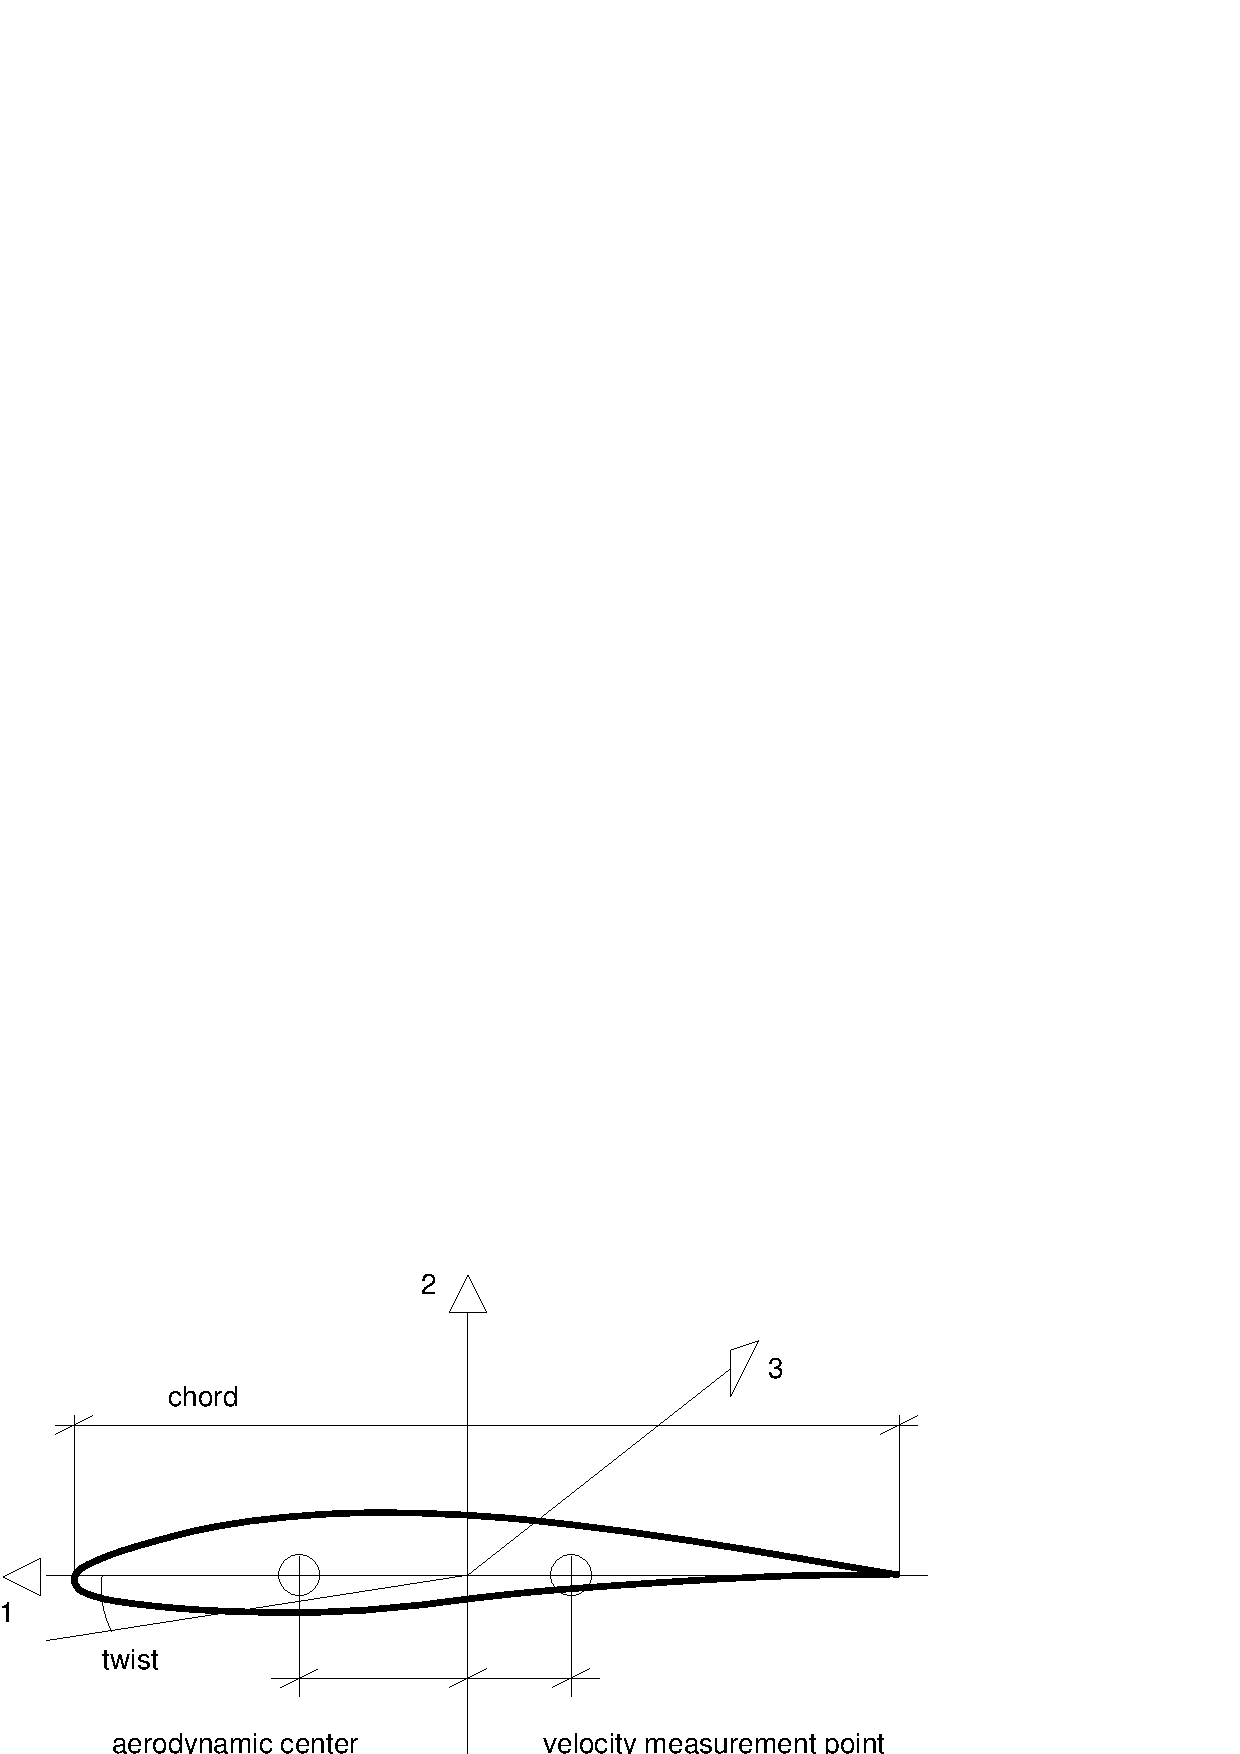
\includegraphics[width=80mm]{airfoil.pdf}
    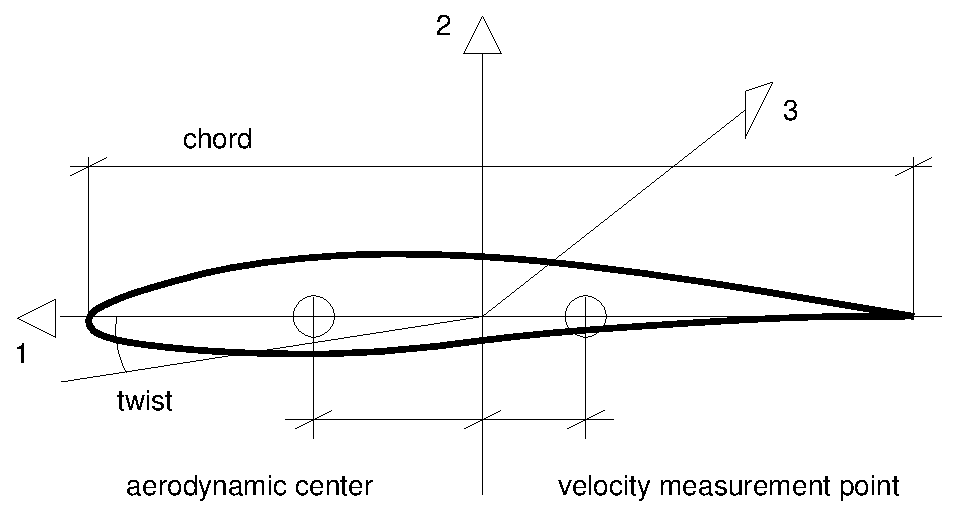
\includegraphics[width=80mm]{airfoil.eps}
  \caption{Airfoil geometry}\label{fig:AIRFOIL}
\end{figure}

The \nt{airfoil\_data} defaults to a built-in NACA 0012 semi-analytical
model (FIXME: the unsteady correction is buggy; use the \kw{c81} 
mode instead).

The \kw{multiple} mode of the c81 data allows to specify
more than one airfoil for an aerodynamic element; the transition
between airfoils is sharp.
The integer \nt{airfoil\_number} indicates how many airfoils are expected;
the real \nt{end\_point} indicates where the influence zone for that
airfoil ends, expressed in terms of a non-dimensional abscissa spanning 
$\plbr{-1,1}$ along the reference line, roughly along axis 3 
of the aerodynamic reference frame; \nt{end\_point} must not lie outside
the element.
So, for example, if airfoil NACA 0015 is used in the leftmost part
of an element up to 1/4 span, NACA 0012 is used from 1/4 to 3/4 span,
and NACA 0009 is used in the remaining rightmost 1/4, the syntax is:
\begin{verbatim}
    set: integer naca0015 = 15;
    set: integer naca0012 = 12;
    set: integer naca0009 = 9;
    c81 data: naca0015, "naca0015.c81";
    c81 data: naca0012, "naca0012.c81";
    c81 data: naca0009, "naca0009.c81";
    # beginning of aerodynamic element definition...
        multiple, 3,
            naca0015, -0.5,    # from -1.0 to -0.5
            naca0012,  0.5,    # from -0.5 to  0.5
            naca0009,  1.0,    # from  0.5 to  1.0
    # ...rest of aerodynamic element definition
\end{verbatim}

The \kw{interpolated} mode of the \kw{c81} data allows to specify 
a smooth transition between different airfoils inside an element.
The interpolation occurs at the integration points where the
aerodynamic data is required, and it is performed once for all
at the beginning of the analysis.
Since this operation is time consuming, and essentially unnecessary,
the interpolated data can be generated once for all with the utility
\texttt{util/c81merge} once the position of the integration point is known,
and the \kw{multiple} mode can be used to directly provide
the interpolated data to the aerodynamic element.

The \kw{theodorsen} aerodynamic data uses C81 data,
and superimposes Wagner's approximation of the Theodorsen incompressible
unsteady correction of 2D lift and moment coefficients.
It is experimental.

The \nt{extra\_arglist} allows to define the style of the output.
The \kw{std} style (the default), the \kw{gauss} and the \kw{node}
styles are illustrated in the output section.


\subsubsection{Output}
Aerodynamic elements, both bodies and beams, write their output with file
extension \texttt{.aer}; for each time step the required elements are output.
In any case the label of the element is output first.
Three different formats are available: \kw{std} (the default),
\kw{gauss} and \kw{node}.

\begin{itemize}
\item[\kw{std}] (or Coefficients at Gauss points):
the output consists in a set of 8 numbers
for each block, that describe data at each Gauss integration point;
multiple blocks for a single element are written on the same line.
The format is:
\begin{itemize}
    \item the angle of attack at that station, in degrees 
	(namely, the angle between the component of the airfoil velocity,
	evaluated at the velocity measurement point, that in the airfoil
	plane and a reference line on the airfoil)
    \item the local yaw angle, in degrees
	(namely, the angle whose tangent is the ratio
	between the axial and the inplane components of the airfoil
	velocity)
    \item the local Mach number
    \item the local lift coefficient
    \item the local drag coefficient
    \item the local aerodynamic moment coefficient
    \item a private number
    \item another private number
\end{itemize}
When \kw{aerodynamic beam2} and \kw{aerodynamic beam3} elements are considered,
the output is repeated for each portion of the beam; so, for example,
a two-node beam is split in two portions, so the output
contains $2\times \nt{integration\_points}$ data blocks,
while a three-node beam is split in three portions,
so the output contains $3\times \nt{integration\_points}$ data blocks.

\item[\kw{node}:]
the format is:
\begin{itemize}
    \item the label of the node
    \item the three components of the force applied to the node
    \item the three components of the couple applied to the node
\end{itemize}
When \kw{aerodynamic beam2} and \kw{aerodynamic beam3} elements are considered,
the output is repeated on the same line for each node
the element is connected to.

\item[\kw{gauss}] (or Forces at Gauss points):
the output consists in the forces and moments
per unit length at each Gauss integration point; the format is:
\begin{itemize}
    \item the direction of the wind velocity relative to the element frame
    \item the lift,
    \item the drag,
    \item and the aerodynamic moment per unit length
\end{itemize}
When \kw{aerodynamic beam2} \and \kw{aerodynamic beam3} elements are considered,
the output is repeated on the same line for each portion of beam.
\end{itemize}



\subsection{Aeromodal Element}
\emph{Note: prepared by Alessandro Scotti.}

\noindent
This element is used to model an aerodynamic modal element,
i.e.\ an unsteady aerodynamic model that inherits the structural 
motion from a  \htmlref{\kw{modal}}{sec:EL:STRUCT:JOINT:MODAL} element
Its definition is very similar to that of the pure modal element, 
but it also includes some data representing unsteady aerodynamics 
in the time domain trough the residualization matrices.
This element is defined as follows:
%\begin{verbatim}
\begin{Verbatim}[commandchars=\\\{\}]
    \bnt{elem_type} ::= \kw{aeromodal}

    \bnt{normal_arglist} ::= 
        \bnt{reference_modal_joint} ,
        (\ty{OrientationMatrix}) \bnt{orientation} ,
        \bnt{reference_chord} ,
        \bnt{number_of_aerodynamic_states} ,
        [ \kw{rigid} , ]
        " \bnt{modal_matrices_file} "
\end{Verbatim}
%\end{verbatim}
With this formulation, anytime an aeromodal element is defined, 
the user needs to declare the number of modal aerodynamic elements 
in use in the \kw{control data} section.
An \htmlref{\kw{air properties}}{sec:EL:AERO:AIRPROPERTIES}
card definition is also required.

The keyword \kw{rigid} indicates that the generalized aerodynamic forces
provided by the model include global forces and moments associated 
to the rigid body motion of the underlying modal element (FIXME: untested).

There is also an optional gust model which is totally undocumented;
for further information, please contact the Author(s).

The \nt{modal\_matrices\_file} file includes the state space model in form 
of matrices $\T{A}$, $\T{B}$, $\T{C}$, $\T{D}_0$, $\T{D}_1$ and $\T{D}_2$,
according to the representation
\begin{align*}
	\dot{\T{x}} &= \T{A}\T{x} + \T{B}\T{q} \\	
	\T{f} &= q\plbr{\T{C}\T{x} + \T{D}_0 \T{q} + \frac{2V_{\infty}}{c} \T{D}_1 \dot{\T{q}} + \plbr{\frac{2V_{\infty}}{c}}^2 \T{D}_2 \ddot{\T{q}}}
\end{align*}
where $\T{q}$ are the modal variables that describe the structural motion,
and $\T{f}$ are the unsteady aerodynamic forces that apply to the structural
dynamics equations.

The file is formatted as follows:
%\begin{verbatim}
\begin{Verbatim}[commandchars=\\\{\}]
    *** MATRIX A
    (\bnt{na} x \bnt{na} coefficients)
    *** MATRIX B
    (\bnt{na} x \bnt{ns} coefficients)
    *** MATRIX C
    (\bnt{ns} x \bnt{na} coefficients)
    *** MATRIX D0
    (\bnt{ns} x \bnt{ns} coefficients)
    *** MATRIX D1
    (\bnt{ns} x \bnt{ns} coefficients)
    *** MATRIX D2
    (\bnt{ns} x \bnt{ns} coefficients)
\end{Verbatim}
%\end{verbatim}

\paragraph{Example.} \
\begin{verbatim}
    aeromodal: WING, WING_JOINT,
        eye,
        131.25, 10, "ha145b.fea";
\end{verbatim}
The \kw{aeromodal} element is declared with the label \texttt{WING}.
This element is attached to a \kw{modal} joint 
named \texttt{WING\_JOINT}.
The orientation of the aerodynamic reference with respect 
to the nodal reference is here expressed by the identity matrix (\kw{eye}).
The aerodynamic element chord is 131.25 inches.
This quantity must be consistent with the system chosen to define 
the whole model (SI, for example; in this case, British Units).
The next field, 10, indicates the number of states needed to use 
the aerodynamic model.
\texttt{ha145b.fea} is the name of the file that contains
the state space model matrices, obtained with an approximation 
chosen by the user.
In this particular case, a 10 states Pad\'e approximation 
has been chosen.
This example is taken from the Bisplinghoff Ashley Halfman
(BAH) Jet Transport Wing cantilevered wing with modal aerodynamic 
frequency responce, computed by a double-lattice method at Mach 0.0.
Data were extracted from the MSC-NASTRAN aeroelastic example file, 
named \texttt{ha145b}, while the aerodynamic state-space fitting 
has been computed using a Pad\'e polynomial approximation
(by Pasinetti \& Mantegazza).
All quantities are expressed in inches and pounds.



\subsection{Aircraft Instruments}
%\begin{verbatim}
\begin{Verbatim}[commandchars=\\\{\}]
    \bnt{elem_type} ::= \kw{aircraft instruments}

    \bnt{normal_arglist} ::= \bnt{aircraft_node}
        [ , \kw{orientation} , (\ty{OrientationMatrix}) \bnt{relative_orientation} ]
\end{Verbatim}
%\end{verbatim}
The \nt{aircraft\_node} represents the aircraft; it is assumed
that the ``nose'' of the aircraft is toward the positive $x$ direction
of the node, and the ``top'' of the aircraft is toward the positive 
$z$ direction of the node.
An optional orientation can be added to change the orientation 
of the aircraft with respect to the node.
This is useful, for example, with helicopters, where conventionally
the positive direction of the $x$ axis is nose to tail.

The available measures are accessed during the simulation 
by defining appropriate \kw{parameter} nodes, and by binding
the \kw{aircraft instruments} element private data to the nodes 
by means of the \kw{bind} mechanism, or directly by means
of the 
\hyperref{\kw{element} drive}{\kw{element} drive (see Section~}{)}{sec:DRIVE:ELEMENT}.

\paragraph{Private Data}
The following data is available:
\begin{itemize}
\item \kw{"airspeed"} the airspeed as seen by the reference 
	point on the aircraft, i.e. the combination 
	of the airstream speed and of the node speed
\item \kw{"groundspeed"} the absolute value of the projection
	of the node speed in the $xy$ plane.
\item \kw{"altitude"} the $z$ component of the node position
\item \kw{"attitude"} $\tan^{-1}\plbr{r_{31}, r_{11}}$
	(FIXME: better $\arcsin\plbr{r_{31}}$?)
\item \kw{"bank"} $\tan^{-1}\plbr{r_{32}, r_{22}}$
	(FIXME: better $\arcsin\plbr{r_{32}}$?)
\item \kw{"turn"} (not available yet)
\item \kw{"slip"} (not available yet)
\item \kw{"verticalspeed"} the $z$ component of the node velocity
\item \kw{"angleofattack"} the angle between the $z$ 
\item \kw{"heading"} the angle between the $x$ axis of the aircraft 
	and the ``north'' (the global $x$ axis) about the global $z$ axis;
	note: heading wraps about South
	(+180 deg from East, -180 deg from West).
\item \kw{"longitude"} (FIXME: not implemented yet)
\item \kw{"latitude"} (FIXME: not implemented yet)
\end{itemize}

\noindent
\emph{Note: this element is eXperimental.}




\subsection{Air Properties}\label{sec:EL:AERO:AIRPROPERTIES}
The properties of the airstream are made of the physical properties
of the air plus the description of the airstream velocity direction
and amplitude.
The former can be expressed in different forms, while the latter
are based on three-dimensional drive callers, \ty{TplDriveCaller<Vec3>}.
%\begin{verbatim}
\begin{Verbatim}[commandchars=\\\{\}]
    \bnt{arglist} ::=
        \{ (\ty{DriveCaller}) \bnt{air_density} , (\ty{Scalar}) \bnt{sound_celerity}
            | \kw{std} , \{ \{ \kw{SI} | \kw{British} \}
                [ , \kw{temperature deviation} , \bnt{delta_T} ]
                | \bnt{p0} , (\ty{DriveCaller}) \bnt{rho0} ,
                    \bnt{T0} , \bnt{dT/dz} , \bnt{R} , \bnt{g0} , \bnt{z1} , \bnt{z2} \}
            [ , \kw{reference altitude} , \bnt{z0} ] \} ,
        (\ty{TplDriveCaller<Vec3>}) \bnt{air_speed}
        [ , \kw{gust} , \bnt{gust_model} [ , ... ] ]
\end{Verbatim}
%\end{verbatim}
The first form consists in the bare input of the air density,
in form of a drive caller, and of the sound celerity, e.g.:
\begin{verbatim}
    air properties: 1.225, 340.,
        1.,0.,0., 150.;
\end{verbatim}
The second form uses standard air properties, both in the
international system (SI) or in British units, possibly
with a temperature deviation and an altitude offset, e.g.:
\begin{verbatim}
    air properties: std, SI, temperature deviation, -55,
        reference altitude, 1000.,
        1.,0.,0., 150.;
\end{verbatim}
where standard properties in SI are used, with a temperature
deviation of -55 K and a reference altitude of 1000 m.
The air properties are computed based on the $z$ position of the
point where the \kw{air properties} are requested (plus the optional
altitude offset).
The last possibility lets the user input all the parameters
required to compute the \kw{air properties} based on the $z$ position
of the point where they are requested, namely the reference
pressure \nt{p0}, the reference density \nt{rho0},
the reference temperature \nt{T0}, the initial temperature
gradient \nt{dT/dz}, the gas constant \nt{R}, the
initial gravity acceleration \nt{g0}, the bottom and top
altitudes of the null temperature gradient region \nt{z1} and
\nt{z2}; e.g., for SI units:
\begin{verbatim}
    air properties: std,
        101325.,       /* Pa */
        1.2250,        /* kg/m^3 */
        288.16,        /* K */
        -6.5e-3,       /* K/m */
        287.,          /* J/kgK */
        9.81,          /* m/s^2 */
        11000.,        /* m */
        25000.,        /* m */
        temperature deviation, -55,
        reference altitude, 1000.,
        1.,0.,0., 150.;
\end{verbatim}
The asymptotic air properties are characterized by the \ty{TplDriveCaller<Vec3>}
of the air speed, in the global reference frame.

\subsubsection{Gust}
If the optional \kw{gust} keyword is used, a gust model can be added.
Note that a very elementary gust model, represented by a uniform change
in airstream speed and direction can be implemented by using
a time-dependent airstream drive.

Gusts can also be appended later to the \kw{air properties} element
by using the statement
%\begin{verbatim}
\begin{Verbatim}[commandchars=\\\{\}]
    \kw{gust} : \bnt{gust_model} ;
\end{Verbatim}
%\end{verbatim}


\paragraph{Front 1D Gust}
The syntax of the \kw{front 1D} gust model is:
%\begin{verbatim}
\begin{Verbatim}[commandchars=\\\{\}]
    \bnt{gust_model} ::= \kw{front 1D} ,
        (\ty{Vec3})        \bnt{front_direction} ,
        (\ty{Vec3})        \bnt{perturbation_direction} ,
        (\ty{Scalar})      \bnt{front_velocity} ,
        (\ty{DriveCaller}) \bnt{front_profile}
\end{Verbatim}
%\end{verbatim}
This model consists in a uniform front, defined as
\begin{displaymath}
	\T{v}\plbr{\T{x}, t} = \T{n} g\plbr{\T{f} \cdot \T{x} + V_{ref} \cdot t}
\end{displaymath}
where
\begin{itemize}
\item $\T{v}$ is the velocity perturbation;
\item $\T{x}$ is the position of the point whose airstream velocity
is being computed;
\item $t$ is the current time;
\item $\T{n}$ is the unit vector \nt{perturbation\_direction} 
that defines the direction of the velocity perturbation;
\item $g\plbr{\cdot}$ is the function \nt{front\_profile} 
that defines the gust profile;
\item $\T{f}$ is the unit vector \nt{front\_direction} 
that defines the direction of propagation of the front;
\item $V_{ref}$ is the velocity \nt{front\_velocity} 
of propagation of the front in direction $\T{f}$.
\end{itemize}
As an example, a transverse cosine-shaped gust, with a wavelength of 100 m
and a peak velocity of 5 m/s moving downstream at the airstream speed,
100 m/s, in standard air, is presented:
\begin{verbatim}
    set: real waveLength = 100.; # m
    set: real V_inf = 100.;      # m/s
    set: real V_g = 5.;          # m/s
    air properties: std, SI,
        1.,0.,0., const, V_inf,  # reference airstream along X
        gust, front 1D,
            1.,0.,0.,            # front moving along X
            0.,0.,1.,            # gust along Z
            V_inf,               # front moving at V_inf
            cosine, 0., pi/waveLength, V_g/2., one, 0.;
\end{verbatim}



\paragraph{Scalar Function Wind Profile}
The syntax of the \kw{scalar function} wind profile,
implemented as a gust model within the \kw{air properties}, is:
%\begin{verbatim}
\begin{Verbatim}[commandchars=\\\{\}]
    \bnt{gust_model} ::= \kw{scalar function} ,
        \kw{reference position} , (\ty{Vec3}) \bnt{X0} ,
        \kw{reference orientation} , (\ty{OrientationMatrix}) \bnt{R0} ,
        (\ty{ScalarFunction}) \bnt{sf}
\end{Verbatim}
%\end{verbatim}
It yields a uniform velocity profile along the $x$ axis of the
reference orientation as a function of the $z$ axis component
of the relative position; namely, given the relative position
\begin{align}
	z &= \T{e}_3 \cdot \plbr{\T{x} - \nt{X0}}
	,
\end{align}
the velocity is
\begin{align}
	\T{v}
	&=
	\T{e}_1 \cdot \nt{sf}(z)
	,
\end{align}
where $\T{e}_i$ is the $i$-th axis of the reference orientation \nt{R0}.



\paragraph{Power Law Wind Profile}
The syntax of the \kw{power law} wind profile, implemented as a gust model
within the \kw{air properties}, is:
%\begin{verbatim}
\begin{Verbatim}[commandchars=\\\{\}]
    \bnt{gust_model} ::= \kw{power law} ,
        \kw{reference position} , (\ty{Vec3}) \bnt{X0} ,
        \kw{reference orientation} , (\ty{OrientationMatrix}) \bnt{R0} ,
        \kw{reference elevation} , \bnt{z_ref} ,
        \kw{reference velocity} , (\ty{DriveCaller}) \bnt{v_ref} ,
        \kw{exponent} , \bnt{exponent}
\end{Verbatim}
%\end{verbatim}
It yields a uniform velocity profile along the $x$ axis of the
reference orientation as a function of the $z$ axis component
of the relative position; namely, given the relative position
\begin{align}
	z &= \T{e}_3 \cdot \plbr{\T{x} - \nt{X0}}
	,
\end{align}
the velocity is
\begin{align}
	\T{v}
	&=
	\T{e}_1 \cdot \nt{v\_ref} \plbr{\frac{z}{\nt{z\_ref}}}^{\nt{exponent}}
	,
\end{align}
where $\T{e}_i$ is the $i$-th axis of the reference orientation \nt{R0}.
Typical values of \nt{exponent} are about 0.1.



\paragraph{Logarithmic Wind Profile}
The syntax of the \kw{logarithmic} wind profile, implemented as a gust model
within the \kw{air properties}, is:
%\begin{verbatim}
\begin{Verbatim}[commandchars=\\\{\}]
    \bnt{gust_model} ::= \kw{logarithmic} ,
        \kw{reference position} , (\ty{Vec3}) \bnt{X0} ,
        \kw{reference orientation} , (\ty{OrientationMatrix}) \bnt{R0} ,
        \kw{reference elevation} , \bnt{z_ref} ,
        \kw{reference velocity} , (\ty{DriveCaller}) \bnt{v_ref} ,
        \kw{surface roughness length} , \bnt{z_0}
\end{Verbatim}
%\end{verbatim}
It yields a uniform velocity profile along the $x$ axis of the
reference orientation as a function of the $z$ axis component
of the relative position; namely, given the relative position
\begin{align}
	z &= \T{e}_3 \cdot \plbr{\T{x} - \nt{X0}}
	,
\end{align}
the velocity is
\begin{align}
	\T{v}
	&=
	\T{e}_1 \cdot \nt{v\_ref} \cdot \frac{
		\log(z/\nt{z\_0}) - \psi_m
	}{
		\log(\nt{z\_ref}/\nt{z\_0}) - \psi_m
	}
	,
\end{align}
where $\T{e}_i$ is the $i$-th axis of the reference orientation \nt{R0}.

The surface roughness length describes the typical roughness
of the surrounding surface.
It is a very small number in case of smooth surface
(e.g.\ 0.01m for grass),
or 1/20 to 1/30 of the typical obstacle's size (e.g.\ 1m for woods).


\paragraph{Output}
The output occurs in the \texttt{.air} file, which contains:
\begin{itemize}
\item a fake label, always set to 1
\item the air density
\item the sound celerity
\item the three components of the reference air speed
with respect to the inertial reference frame
\end{itemize}


\paragraph{Private Data}
The following data is available:
\begin{itemize}
\item \kw{"vxinf"} the $x$ component of the airstream speed (without any gust contribution)
\item \kw{"vyinf"} the $y$ component of the airstream speed (without any gust contribution)
\item \kw{"vzinf"} the $z$ component of the airstream speed (without any gust contribution)
\item \kw{"vinf"} the module of the airstream speed (without any gust contribution)
\end{itemize}



\subsection{Generic Aerodynamic Force}
\label{sec:EL:AERO:GAF}
This element is experimental.
%\begin{verbatim}
\begin{Verbatim}[commandchars=\\\{\}]
    \bnt{elem_type} ::= \kw{generic aerodynamic force}

    \bnt{normal_arglist} ::= \bnt{node_label} ,
        [ \kw{position} , \bnt{relative_position} , ]
        [ \kw{orientation} , \bnt{relative_orientation} , ]
        [ \kw{reference surface} , \bnt{reference_surface} , ]
        [ \kw{reference length} , \bnt{reference_length} , ]
        \{ \bnt{data_file_specification} | \kw{reference} , \bnt{gaf_data_label} \}

    \bnt{data_file_specification} ::= \kw{file} , 
        [ \{ \kw{angle units} , \{ \kw{radians} | \kw{degrees} \}
            | \kw{scale angles} , \bnt{angle_scale_factor} \} , ]
        [ \kw{scale lengths} , \bnt{length_scale_factor} , ]
        " \bnt{data_file_name} "
\end{Verbatim}
%\end{verbatim}

\paragraph{Output}
The following output is available:
\begin{enumerate}
\item column 1: element label
\item column 2: the angle of attack $\alpha$
\item column 3: the sideslip angle $\beta$
\item columns 4--6: force components in local $x$, $y$ and $z$ directions
\item columns 7--9: moment components in local $x$, $y$ and $z$ directions,
	about the reference point (node plus offset)
\item columns 10--12: force components in global $x$, $y$ and $z$ directions
\item columns 13--15: moment components in global $x$, $y$ and $z$ directions,
	about the node
\end{enumerate}

\paragraph{Private Data}
The \kw{generic aerodynamic force} element does not output any private data.

\subsubsection{Generic Aerodynamic Element Data}
Data is stored in ASCII format in a file.

An arbitrary number of comment lines is allowed at the beginning.
Comment lines start with either a percent `\textbf{\%}'
or a hash mark `\texttt{\#}' in the first column.
Their content is discarded until the end of the line.

The first non-comment line must contain two integers separated by whitespace.
The integers represent the expected number of angle of attack
and sideslip angle values, $N_\alpha$ and $N_\beta$.

Another arbitrary number of comment lines is allowed.

A set of $N_\alpha \cdot N_\beta$ lines is expected.
No comments or empty lines are allowed in between.
Each line contains:
\begin{itemize}
\item column 1: the angle of attack, $\alpha$
\item column 2: the sideslip angle, $\beta$
\item columns 3--5: the force coefficients $f_{x/q}$, $f_{y/q}$, $f_{z/q}$
\item columns 6--8: the moment coefficients $m_{x/q}$, $m_{y/q}$, $m_{z/q}$
\end{itemize}

Notes:
\begin{enumerate}
\item lines are sorted as follows:
all values of $\alpha$ are defined for each value of $\beta$;
the same values of $\alpha$ are expected for each value of $\beta$;
\item the angle ranges are $-\pi/2 \le \alpha \le \pi/2$,
$-\pi \le \beta \le \pi$;
\item the angles are expected in radians;
use the mutually exclusive optional keywords \kw{angle units},
to specify either \kw{radians} or \kw{degrees},
or \kw{scale angles}, to specify the \nt{angle\_scale\_factor};
\item $q=1/2 \rho V^2$ is the local reference dynamic pressure,
where $V$ is the norm of the velocity at the reference point;
\item the coefficients express forces and moments in the reference frame
attached to the body;
\item the coefficients are either expected in dimensional
or non-dimensional form.
In the former case, the force coefficients represent areas,
while the moment coefficients represent volumes, since they need
to be multiplied by the dynamic pressure to become forces and moments.
In the latter case, they are pure numbers;
a reference surface and length must be defined in the configuration
of the corresponding \kw{generic aerodynamic force} element.
When dimensional coefficients are specified, they can be rescaled
by using the optional keyword \kw{scale lengths} to specify
the \nt{length\_scale\_factor}.
\end{enumerate}

\paragraph{Example.}
The content of the file \texttt{example.dat} is
\begin{verbatim}
# This is an example of data for the "generic aerodynamic force" element
# 5 values of angle of attack (alpha) and 4 values of sideslip angle (beta)
# are provided
5 4
# alpha beta fx/q fy/q fz/q mx/q my/q mz/q
-90 -180  0  0  0  0  0  0
-20 -180  0  0  0  0  0  0
  0 -180  0  0  0  0  0  0
 20 -180  0  0  0  0  0  0
 90 -180  0  0  0  0  0  0
-90  -20  0  0  0  0  0  0
-20  -20  0  0  0  0  0  0
  0  -20  0  0  0  0  0  0
 20  -20  0  0  0  0  0  0
 90  -20  0  0  0  0  0  0
-90   20  0  0  0  0  0  0
-20   20  0  0  0  0  0  0
  0   20  0  0  0  0  0  0
 20   20  0  0  0  0  0  0
 90   20  0  0  0  0  0  0
-90  180  0  0  0  0  0  0
-20  180  0  0  0  0  0  0
  0  180  0  0  0  0  0  0
 20  180  0  0  0  0  0  0
 90  180  0  0  0  0  0  0
\end{verbatim}
The corresponding statement in the input file is
\begin{verbatim}
    set: integer GAF_NODE = 10;
    set: integer GAF_ELEM = 20;
    generic aerodynamic force: GAF_ELEM, GAF_NODE,
        file, angle units, degrees, "example.dat";
\end{verbatim}



\subsection{Induced velocity}
\label{sec:EL:AERO:INDVEL}
The \kw{induced velocity} element is used to associate the aerodynamic elements
that model the lifting surfaces of an aircraft,
or the blades of a helicopter rotor, when some inflow related computations 
are required.

By means of different inflow models, and by means
of the aerodynamic load contributions supplied by the aerodynamic elements,
the \kw{induced velocity} element is able to compute the induced velocity
at an arbitrary point on the lifting surface or rotor disk.
This velocity term in turn is used by the aerodynamic elements to determine
a better estimate of the boundary conditions.

The syntax of the \kw{induced velocity} elements is:
%\begin{verbatim}
\begin{Verbatim}[commandchars=\\\{\}]
    \bnt{elem_type} ::= \kw{induced velocity}

    \bnt{normal_arglist} ::= \bnt{induced_velocity_type} , \bnt{induced_velocity_data}
\end{Verbatim}
%\end{verbatim}

\subsubsection{Rotor}
\label{sec:EL:AERO:INDVEL:ROTOR}
Currently, induced velocity models are only implemented
for helicopter rotors.
Originally, this type of element was known as \kw{rotor},
and the original syntax is preserved for backwards compatibility.

The syntax of the helicopter rotor \kw{induced velocity} element is:
%\begin{verbatim}
\begin{Verbatim}[commandchars=\\\{\}]
    \bnt{induced_velocity_type} ::= \kw{rotor}

    \bnt{induced_velocity_data} ::= \bnt{craft_node} ,
            [ \kw{orientation} , (\ty{OrientationMatrix}) \bnt{rotor_orientation} , ]
        \bnt{rotor_node} ,
        \kw{induced velocity} , \bnt{induced_velocity_model}
\end{Verbatim}
%\end{verbatim}
The optional \nt{rotor\_orientation} is required when axis 3 
of the \nt{craft\_node} is not aligned with the rotor axis; axis 3
of the \nt{rotor\_node} must be aligned with the rotor axis.

There are five models of induced velocity. 
The first is no induced velocity; the syntax is:
%\begin{verbatim}
\begin{Verbatim}[commandchars=\\\{\}]
    \bnt{induced_velocity_model} ::= \kw{no}
\end{Verbatim}
%\end{verbatim}
There is no argument list. This element does not compute any induced
velocity, but still computes the rotor traction for output purposes,
if output is required.
The others have a fairly common syntax.  The first three are
\kw{uniform}, \kw{glauert} and \kw{mangler} induced velocity
models:
%\begin{verbatim}
\begin{Verbatim}[commandchars=\\\{\}]
    \bnt{induced_velocity_model} ::= \{ \kw{uniform} | \kw{glauert} | \kw{mangler} \} , 
        \bnt{reference_omega} , \bnt{reference_radius}
        [ , \bnt{option} [ , ... ] ]

    \bnt{option} ::=
        \{ \kw{ground} , \bnt{ground_node}
            | \kw{delay} , (\ty{DriveCaller}) \bnt{memory_factor}
            | \kw{max iterations} , \bnt{max_iterations}
            | \kw{tolerance} , \bnt{tolerance}
            | \kw{eta} , \bnt{eta}
            | \kw{correction} , \bnt{hover_correction_factor}, \bnt{ff_correction_factor} \}
\end{Verbatim}
%\end{verbatim}

\begin{itemize}
\item
The \nt{reference\_omega} field is used to decide whether
the induced velocity computation must be inhibited because the rotor speed
is very low.

\item
The \nt{reference\_radius} field is used to make the rotor related parameters
non-dimensional.

\item
The \kw{ground} parameter is used to inform the rotor about the proximity
to the ground; the $z$ component of the distance between the rotor
and the ground nodes, in the ground node reference frame
(direction 3, positive),
is used for an approximate correction of the axial inflow velocity
\cite{NASA-TR-3021}.

\item
The \nt{memory\_factor}, the \nt{hover\_correction\_factor} 
and the \nt{ff\_correction\_factor} (forward flight) are
used to correct the nominal induced velocity, according to the formula
\begin{align*}
	U_{\text{effective}}
	&=
	\plbr{1 - \nt{memory\_factor}} U_{\text{nominal}}
	\\
	&+ \nt{memory\_factor} \ U_{\text{previous}}
\end{align*}
with
\begin{align*}
	U_{\text{nominal}}
	&=
	\frac{T}{2 \rho A V_{\text{tip}} \sqrt{
		\cfrac{\lambda^2}{\nt{hover\_correction\_factor}^4}
		+ \cfrac{\mu^2}{\nt{ff\_correction\_factor}^2}
	}}
\end{align*}
The \kw{delay} parameter is used to linearly combine the current
reference induced velocity with the induced velocity at the previous step;
no delay means there is no memory of the previous value.
The memory factor behaves like a discrete first-order low-pass filter.
As a consequence, its behavior depends on the integration time step.
The \nt{memory\_factor} parameter defaults to 0.
The \nt{hover\_correction\_factor} 
and \nt{ff\_correction\_factor} parameters default to 1.

\item
The \nt{max\_iterations}, \nt{tolerance} 
and \nt{eta} parameters refer to the iteration cycle 
that is performed to compute the nominal induced velocity.
After \nt{max\_iterations}, or when the absolute value 
of the difference between two iterations of the nominal induced 
velocity is less than \nt{tolerance}, the cycle ends.
Only a fraction \nt{eta} of the difference between two
iterations of the nominal induced velocity is actually
used; \nt{eta} defaults to 1.
The default is to make only one iteration, which is backward-compatible
with the original behavior.
\end{itemize}

The last induced velocity model uses a dynamic inflow model,
based on \cite{PITT}, with 3 inflow states.
The syntax is:
%\begin{verbatim}
\begin{Verbatim}[commandchars=\\\{\}]
    \bnt{induced_velocity_model} ::= \kw{dynamic inflow} , 
        \bnt{reference_omega} , 
        \bnt{reference_radius} 
        [ , \bnt{option} [ , ... ] ]

    \bnt{option} ::=
        \{ \kw{ground} , \bnt{<ground_node}
            | \kw{initial value} , \bnt{const_vel} , \bnt{cosine_vel} , \bnt{sine_vel}
            | \kw{max iterations} , \bnt{max_iterations}
            | \kw{tolerance} , \bnt{tolerance}
            | \kw{eta} , \bnt{eta}
            | \kw{correction} , \bnt{hover_correction_factor} , \bnt{ff_correction_factor} \}
\end{Verbatim}
%\end{verbatim}
Most of the parameters are the same as for the previous models.
The optional \kw{delay} parameter is no longer allowed.
The three states, corresponding to uniform, fore-aft and lateral inflow,
can be explicitly initialized by means of the optional 
\kw{initial value} parameter.

\paragraph{Output}
The following output is available for all rotor elements:
\begin{enumerate}
\item column 1: element label
\item columns 2--4: rotor force in $x$, $y$ and $z$ directions
	(longitudinal, lateral and thrust components)
\item columns 5--7: rotor moment about $x$, $y$ and $z$ directions
	(roll, pitch and torque components)
\item column 8: mean inflow velocity, based on momentum theory
\item column 9: reference velocity at rotor center, sum of airstream
	and \nt{craft\_node} node velocity
\item column 10: rotor disk angle
\item column 11: advance parameter $\mu$
\item column 12: inflow parameter $\lambda$
\item column 13: advance/inflow angle $\chi=\tan^{-1}\plbr{\mu/\lambda}$
\item column 14: reference azimuthal direction $\psi_0$,
	related to rotor yaw angle
\item column 15: boolean flag indicating convergence
	in reference induced velocity computation internal iterations
\item column 16: number of iterations required for convergence
\newcounter{elem_rotor_output}
\setcounter{elem_rotor_output}{\value{enumi}}
\end{enumerate}
The \kw{dynamic inflow} model adds the columns
\begin{enumerate}
\setcounter{enumi}{\value{elem_rotor_output}}
\item column 17: constant inflow state
\item column 18: sine inflow state (lateral)
\item column 19: cosine inflow state (longitudinal)
\end{enumerate}
Rotor force and moment (columns 2--4 and 5--7) are the aerodynamic
force and moment exerted by the rotor aerodynamics on the \nt{rotor\_node},
projected in the reference frame of the \nt{craft\_node},
optionally modified by the \nt{rotor\_orientation} matrix.
The conventional naming of longitudinal (or drag), lateral and thrust force,
and roll, pitch and torque moment, refer to a rotorcraft
whose $x$ axis is the longitudinal (nose to tail) axis,
whose $y$ axis is the lateral (portside) axis,
and whose $z$ axis is the vertical (bottom to top) axis.

\paragraph{Private Data}
The following data is available:
\begin{enumerate}
\item \kw{"Tx"} rotor force in $x$ direction (longitudinal force)
\item \kw{"Ty"} rotor force in $y$ direction (lateral force)
\item \kw{"Tz"} rotor force in $z$ direction (thrust)
\item \kw{"Mx"} rotor moment about $x$ direction (roll moment)
\item \kw{"My"} rotor moment about $y$ direction (pitch moment)
\item \kw{"Mz"} rotor moment about $z$ direction (torque)
\end{enumerate}
The rotor force and moment components are expressed in the same reference
frame described in the Output Section above.



\subsection{Rotor}
\label{sec:EL:AERO:ROTOR}
Deprecated; see \kw{induced velocity} (Section~\ref{sec:EL:AERO:INDVEL:ROTOR}).





\section{Automatic structural}
The so called \kw{automatic structural} element is automatically generated
when a dynamic structural node is instantiated.
As such, when defined in the \kw{elements} block,
the element already exists.
The only reason to repeat its definition is to modify the values
of the momentum and of the momenta moment, and to initialize
their derivatives.
The label must match that of the node it refers to.
%\begin{verbatim}
\begin{Verbatim}[commandchars=\\\{\}]
    \bnt{elem_type} ::= \kw{automatic structural}

    \bnt{normal_arglist} ::=
        (\ty{Vec3}) \bnt{momentum} ,
        (\ty{Vec3}) \bnt{momenta_moment} ,
        (\ty{Vec3}) \bnt{momentum_derivative} ,
        (\ty{Vec3}) \bnt{momenta_moment_derivative}
\end{Verbatim}
%\end{verbatim}
All the provided values are recomputed during the initial derivatives phase,
so they should be intended as initial values for the Newton iteration.
In general, there is no need to provide this data; they can speed up
initial convergence in case of systems that are not at rest in the initial
configuration, with kinematic constraints that strongly affect
the motion.

\paragraph{Private Data}
The following data is available:
\begin{enumerate}
\item \kw{"beta[1]"} momentum in global direction 1
\item \kw{"beta[2]"} momentum in global direction 2
\item \kw{"beta[3]"} momentum in global direction 3
\item \kw{"gamma[1]"} momenta moment in global direction 1
\item \kw{"gamma[2]"} momenta moment in global direction 2
\item \kw{"gamma[3]"} momenta moment in global direction 3
\item \kw{"betaP[1]"} momentum derivative in global direction 1
\item \kw{"betaP[2]"} momentum derivative in global direction 2
\item \kw{"betaP[3]"} momentum derivative in global direction 3
\item \kw{"gammaP[1]"} momenta moment derivative in global direction 1
\item \kw{"gammaP[2]"} momenta moment derivative in global direction 2
\item \kw{"gammaP[3]"} momenta moment derivative in global direction 3
\end{enumerate}


% beam element
% $Header$
% MBDyn (C) is a multibody analysis code.
% http://www.mbdyn.org
%
% Copyright (C) 1996-2010
%
% Pierangelo Masarati  <masarati@aero.polimi.it>
%
% Dipartimento di Ingegneria Aerospaziale - Politecnico di Milano
% via La Masa, 34 - 20156 Milano, Italy
% http://www.aero.polimi.it
%
% Changing this copyright notice is forbidden.
%
% This program is free software; you can redistribute it and/or modify
% it under the terms of the GNU General Public License as published by
% the Free Software Foundation (version 2 of the License).
% 
%
% This program is distributed in the hope that it will be useful,
% but WITHOUT ANY WARRANTY; without even the implied warranty of
% MERCHANTABILITY or FITNESS FOR A PARTICULAR PURPOSE.  See the
% GNU General Public License for more details.
%
% You should have received a copy of the GNU General Public License
% along with this program; if not, write to the Free Software
% Foundation, Inc., 59 Temple Place, Suite 330, Boston, MA  02111-1307  USA

\section{Beam Elements}
\label{sec:EL:BEAM}
The family of finite volume beam elements implemented in MBDyn
allows to model slender deformable structural components 
with a high level of flexibility.

The beam is defined by a reference line and by a manifold
of orientations attached to the line.
It is assumed that the direction 1 of the orientations lies along
the reference line, but it is not strictly required to be tangent
to it even in the reference configuration.

The beam element is defined by its nodes; currently, 2 and 3 node 
beam elements are implemented.
Each node of the beam is related to a \kw{structural node} by an offset
and an optional relative orientation, to provide topological flexibility.

The beam element is modeled by means of an original Finite Volume approach
\cite{FV-AIAA}, which computes the internal forces as functions 
of the straining of the reference line and orientation at selected points
along the line itself, called \emph{evaluation points},
which lie somewhere between two pairs of beam nodes.

At each evaluation point, a 6D constitutive law must be defined,
which defines the relationship between the strains, the curvatures
of the beam and their time derivatives
and the internal forces and moments at the evaluation points.

The strains and curvatures and their time derivatives are obtained 
from the nodal positions and orientations by differentiating
the interpolation functions.

The 6D constitutive laws are defined as
\begin{displaymath}
	\cubr{\cvvect{
		F_x \\
		F_y \\
		F_z \\
		M_x \\
		M_y \\
		M_z
	}} = \T{f}\plbr{
		\cubr{\cvvect{
			\varepsilon_x \\
			\gamma_y \\
			\gamma_z \\
			\kappa_x \\
			\kappa_y \\
			\kappa_z
		}},
		\cubr{\cvvect{
			\dot{\varepsilon}_x \\
			\dot{\gamma}_y \\
			\dot{\gamma}_z \\
			\dot{\kappa}_x \\
			\dot{\kappa}_y \\
			\dot{\kappa}_z
		}}
	}
\end{displaymath}
where, if the convention of using $x$ as beam axis is followed:
\begin{itemize}
\item $F_x$ is the axial force component;
\item $F_y$ and $F_z$ are the shear force components;
\item $M_x$ is the torsional moment component;
\item $M_y$ and $M_z$ are the bending moment components;
\item $\varepsilon_x$ is the axial strain component;
\item $\gamma_y$ and $\gamma_z$ are the shear strain components;
\item $\kappa_x$ is the torsional curvature component;
\item $\kappa_y$ and $\kappa_z$ are the bending curvature component;
\item $\T{f}$ is an arbitrary function that defines the constitutive law.
\end{itemize}



\subsection{Beam Section Constitutive Law}
Typically, linear elastic or viscoelastic constitutive laws are used,
although one may want to implement specific nonlinear elastic
or elastic-plastic constitutive laws.



\subsubsection{Beam Section Characterization}
MBDyn allows the broadest generality in defining what a linear elastic 
constitutive law contains, since the entire $6\times{6}$ constitutive
matrix can be input.
This means that internal forces and couples can be arbitrarily related
to generalized strains and curvatures.
However, to make sense, a constitutive matrix at the section level,
must satisfy some constraints, e.g.\ it is expected to be symmetric, 
although this is not strictly enforced by the code.

However, most of the info about the extra-diagonal terms 
of the stiffness matrix are not usually available.
One easy way to work this around is to resort to any so-called
composite beam section characterization analysis available 
in the literature.

For details, the reader is referred to \cite{HODGES-REVIEW90} 
for a review of the topic, to \cite{ANBA-GIAVOTTO-83}
for an early work on the subject, and to \cite{MASARATI-2001}
for a more recent review of the original formulation.
The software that implements this type of analysis is called ANBA++.
It is not free software, so far.
Prospective users can contact the authors, through MBDyn developers.


\subsubsection{Disclaimer}
The following paragraphs are intended as a means to help users
preparing data for MBDyn models in a consistent manner.
By no means they indicate that the beam section stiffness properties
must be provided in a specific reference frame.
On the contrary, MBDyn allows as much generality as possible,
and actually the variety of choices is redundant, since equivalent
properties can be input in different ways.

This is intended to allow the code to suit the users' needs
regardless of the original format of the input data.
As such, all the transformations reported in the following 
are only intended as suggestions and should not be taken literally.
For instance, rotations and offsets of reference points
could be reversed, changing the values of the offsets, without
affecting the final result.

The most important aspect of MBDyn notion of beam section properties
is that the reference point and orientation, although arbitrary,
must be unique, and the common notions of center of axial strain,
shear center (and center of mass) have no special meaning.



\subsubsection{Equivalent $6\times6$ Section of Isotropic Beam}
When an isotropic beam section is considered, the $6\times$ 
constitutive matrix, referred to an arbitrary point in the section,
with an arbitrary orientation, can always be written in terms 
of elementary stiffness and geometrical properties.
These are the properties that are usually available in tabular form
either from simplified beam section analysis or by experiments.
A sketch of a generic section is shown
in Figure~\ref{fig:EL:BEAM:SECTION},
where the arbitrary reference frame indicated by axes 
$x$, $y$ and $z$ originates from an arbitrary reference point
on the section.

Isotropic uniform beam sections allow to group the internal forces 
and couples in two sets, together with their conjugated generalized 
strains:
those related to shear stress and strain, and those related 
to axial stress and strain, as illustrated
in Figure~\ref{fig:EL:BEAM:GROUPS}.
\begin{figure}[h]
\centering
\begin{tabular}{c|c|c|c|c|c|c|}
	&
		$\varepsilon_x$ &
		$\gamma_y$ &
		$\gamma_z$ &
		$\kappa_x$ &
		$\kappa_y$ &
		$\kappa_z$ \\
	\hline
	$F_x$ & A &   &   &   & A & A \\
	\hline
	$F_y$ &   & S & S & S &   &   \\
	\hline
	$F_z$ &   & S & S & S &   &   \\
	\hline
	$M_x$ &   & S & S & S &   &   \\
	\hline
	$M_y$ & A &   &   &   & A & A \\
	\hline
	$M_z$ & A &   &   &   & A & A \\
	\hline
\end{tabular}
\caption{Constitutive coefficients grouping (S: shear, A: axial)}
\label{fig:EL:BEAM:GROUPS}
\end{figure}
There is no direct coupling between the two groups, at the section level,
so the corresponding coupling coefficients are always zero.
This is no longer true when material anisotropy must be taken 
into account.

The $3\times3$ sub-blocks can be separately transformed 
in diagonal form by referring the corresponding properties
to appropriate separate points in the beam section, 
and by applying an appropriate rotation about the axis of the beam.



\subsubsection{Axial Stress and Strain Properties}
This section considers the submatrix represented by the coefficients 
marked as A in Figure~\ref{fig:EL:BEAM:GROUPS}, under the assumption 
that it is symmetric.

First, the problem of obtaining axial stiffness properties referred
to a generic point in a generic orientation is considered,
when the properties referred to the axial strain center
in the principal reference frame are known.

Then, the problem of extracting the location of the axial strain center
and of the principal reference frame, and the principal bending stiffnesses
from generic data is presented as well.

The two problems are complementary.
Usually, the first one needs to be considered when engineering properties
are available and the generic constitutive properties required by MBDyn
need to be computed.

\paragraph{Diagonal to Generic Properties.}
First the transformation from diagonal to generic properties
is considered.
This transformation consists in rotating the section properties
and then in referring them to a common reference point in the blade section.

The diagonal properties are described by the constitutive matrix
\begin{align}
	\cubr{\cvvect{
		F_x \\
		M_y \\
		M_z
	}}^{\dagger}
	&=
	\sqbr{\matr{ccc}{
		EA & 0 & 0 \\
		& EJ_y & 0 \\
		\text{sym.} & & EJ_z
	}} \cubr{\cvvect{
		\varepsilon_x \\
		\kappa_y \\
		\kappa_z
	}} .
\end{align}
This constitutive matrix is expressed in a reference frame that is centered
in the center of axial strain, indicated with the subscript $as$,
and oriented according to the bending principal axes.

A rotation $\alpha$ about axis $x$ is used to transform the properties
into the common reference frame of the beam section.
The internal forces and moments are thus transformed according to 
\begin{align}
	\cubr{\cvvect{
		F_x \\
		M_y \\
		M_z \\
	}}^*
	&=
	\sqbr{R}_{\text{axial}} \cubr{\cvvect{
		F_x \\
		M_y \\
		M_z \\
	}}^{\dagger}
	\nonumber \\
	&=
	\sqbr{\matr{ccc}{
		1 & 0 & 0 \\
		0 & \cos\alpha & -\sin\alpha \\
		0 & \sin\alpha & \cos\alpha
	}} \cubr{\cvvect{
		F_x \\
		M_y \\
		M_z \\
	}}^{\dagger}
	,
\end{align}
while the strains and curvatures are transformed according to
\begin{align}
	\cubr{\cvvect{
		\varepsilon_x \\
		\kappa_y \\
		\kappa_z \\
	}}^*
	&= \sqbr{R}^{-T}_{\text{axial}} \cubr{\cvvect{
		\varepsilon_x \\
		\kappa_y \\
		\kappa_z \\
	}}^{\dagger}
	\nonumber \\
	&= \sqbr{R}_{\text{axial}} \cubr{\cvvect{
		\varepsilon_x \\
		\kappa_y \\
		\kappa_z \\
	}}^{\dagger}
	.
\end{align}
As a consequence, the constitutive relationship becomes
\begin{align}
	\cubr{\cvvect{
		F_x \\
		M_y \\
		M_z \\
	}}^*
	&=
	\sqbr{R}_{\text{axial}} \sqbr{A}^{\dagger} \sqbr{R}_{\text{axial}}^T
	\cubr{\cvvect{
		\varepsilon_x \\
		\kappa_y \\
		\kappa_z \\
	}}^*
	\nonumber \\
	&= \sqbr{\matr{ccc}{
		EA & 0 & 0 \\
		& EJ_y \cos^2\alpha + EJ_z \sin^2\alpha
			& \plbr{EJ_y - EJ_z}\cos\alpha\sin\alpha \\
		\text{sym.} & & EJ_z \cos^2\alpha + EJ_y \sin^2\alpha
	}}
	\cubr{\cvvect{
		\varepsilon_x \\
		\kappa_y \\
		\kappa_z \\
	}}^*
	.
\end{align}

An offset of the reference point results from the internal force
and moment transformation
\begin{align}
	\cubr{\cvvect{
		F_x \\
		M_y \\
		M_z \\
	}}
	&= \sqbr{T}_{\text{axial}} \cubr{\cvvect{
		F_x \\
		M_y \\
		M_z \\
	}}^*
	\nonumber \\
	&=
	\sqbr{\matr{ccc}{
		1 & 0 & 0 \\
		z_{as} & 1 & 0 \\
		-y_{as} & 0 & 1
	}}
	\cubr{\cvvect{
		F_x \\
		M_y \\
		M_z \\
	}}^*
	.
\end{align}
Similarly,
the strains and curvatures are transformed according to the relationship
\begin{align}
	\cubr{\cvvect{
		\varepsilon_x \\
		\kappa_y \\
		\kappa_z \\
	}}
	&=
	\sqbr{T}_{\text{axial}}^{-T}
	\cubr{\cvvect{
		\varepsilon_x \\
		\kappa_y \\
		\kappa_z \\
	}}^*
	.
\end{align}
The constitutive relationship becomes
\begin{align}
	\cubr{\cvvect{
		F_x \\
		M_y \\
		M_z \\
	}}
	&=
	\sqbr{T}_{\text{axial}} \sqbr{A}^* \sqbr{T}_{\text{axial}}^T
	\cubr{\cvvect{
		\varepsilon_x \\
		\kappa_y \\
		\kappa_z \\
	}}
	\nonumber \\
	&= \sqbr{T}_{\text{axial}} \sqbr{R}_{\text{axial}}
		\sqbr{A}^{\dagger}
		\sqbr{R}_{\text{axial}}^T \sqbr{T}_{\text{axial}}^T
	\cubr{\cvvect{
		\varepsilon_x \\
		\kappa_y \\
		\kappa_z \\
	}}
	\nonumber \\
	&=
	\sqbr{\matr{ccc}{
		A_{11} & A_{12} & A_{13} \\
		& A_{22} & A_{23} \\
		\text{sym.} & & A_{33}
	}}
	\cubr{\cvvect{
		\varepsilon_x \\
		\kappa_y \\
		\kappa_z \\
	}}
	.
\end{align}
The values of the coefficients are
\begin{subequations}
\begin{align}
	A_{11} &= EA \\
	A_{12} &= z_{as} EA \\
	A_{13} &= -y_{as} EA \\
	A_{22} &= EJ_y \cos^2\alpha + EJ_z \sin^2\alpha + z_{as}^2 EA \\
	A_{23} &= \plbr{EJ_y - EJ_z}\cos\alpha\sin\alpha - y_{as} z_{as} EA \\
	A_{33} &= EJ_z \cos^2\alpha + EJ_y \sin^2\alpha + y_{as}^2 EA
\end{align}
\end{subequations}



\paragraph{Generic to Diagonal Properties.}
Consider now a generic axial portion of the constitutive properties,
symmetric and usually positive-definite.
The constitutive matrix can be transformed to diagonal form
by moving the reference point by an offset in the plane of the section,
and then by rotating the properties about axis $x$.

The offset is applied by the internal forces and moments transformation
\begin{align}
	\cubr{\cvvect{
		F_x \\
		M_y \\
		M_z
	}}^*
	&=
	\sqbr{T}_{\text{axial}}^{-1}
	\cubr{\cvvect{
		F_x \\
		M_y \\
		M_z
	}}
	\nonumber \\
	&=
	\sqbr{\matr{ccc}{
		1 & 0 & 0 \\
		-z_{as} & 1 & 0 \\
		y_{as} & 0 & 1
	}}
	\cubr{\cvvect{
		F_x \\
		M_y \\
		M_z
	}}
	.
\end{align}
The corresponding strains and curvatures transformation is
\begin{align}
	\cubr{\cvvect{
		\varepsilon_x \\
		\kappa_y \\
		\kappa_z \\
	}}^*
	&=
	\sqbr{T}_{\text{axial}}^T
	\cubr{\cvvect{
		\varepsilon_x \\
		\kappa_y \\
		\kappa_z \\
	}}
	.
\end{align}
The transformed constitutive relationship is
\begin{align}
	\cubr{\cvvect{
		F_x \\
		M_y \\
		M_z
	}}^*
	&=
	\sqbr{T}_{\text{axial}}^{-1} \sqbr{A} \sqbr{T}_{\text{axial}}^{-T}
	\cubr{\cvvect{
		\varepsilon_x \\
		\kappa_y \\
		\kappa_z \\
	}}
	\nonumber \\
	&=
	\sqbr{\matr{ccc}{
		A_{11} & A_{12} - z_{as} A_{11} & A_{13} + y_{as} A_{11} \\
		& A_{22} - 2 z_{as} A_{12} + z_{as}^2 A_{11}
			& A_{23} - z_{as} A_{13} + y_{as} A_{12} - y_{as} z_{as} A_{11} \\
		\text{sym.} & & A_{33} + 2 y_{as} A_{13} + y_{as}^2 A_{11}
	}}
	\cubr{\cvvect{
		\varepsilon_x \\
		\kappa_y \\
		\kappa_z \\
	}}^*
	\label{eq:EL:BEAM:AXIAL:R:*}
	.
\end{align}
The location that decouples the axial force from the bending moments is
\begin{subequations}
\label{eq:EL:BEAM:AXIAL:R:AS}
\begin{align}
	y_{as} &= - \frac{A_{13}}{A_{11}} \\
	z_{as} &= \frac{A_{12}}{A_{11}}
\end{align}
\end{subequations}
When the location of Eq.~(\ref{eq:EL:BEAM:AXIAL:R:AS}) is considered,
Eq.~(\ref{eq:EL:BEAM:AXIAL:R:*}) becomes
\begin{align}
	\cubr{\cvvect{
		F_x \\
		M_y \\
		M_z
	}}^*
	&=
	\sqbr{\matr{ccc}{
		A_{11} & 0 & 0 \\
		& A_{22} - A_{12}^2/A_{11}
			& A_{23} - A_{12} A_{13}/A_{11} \\
		\text{sym.} & & A_{33} - A_{13}^2/A_{11}
	}}
	\cubr{\cvvect{
		\varepsilon_x \\
		\kappa_y \\
		\kappa_z \\
	}}^*
	\nonumber \\
	&=
	\sqbr{\matr{ccc}{
		A_{11}^* & 0 & 0 \\
		& A_{22}^* & A_{23}^* \\
		\text{sym.} & & A_{33}^*
	}}
	\cubr{\cvvect{
		\varepsilon_x \\
		\kappa_y \\
		\kappa_z \\
	}}^*
	.
\end{align}

When a rotation about axis $x$ is considered, the internal forces
and moments are transformed according to the relationship
\begin{align}
	\cubr{\cvvect{
		F_x \\
		M_y \\
		M_z
	}}^{\dagger}
	&= \sqbr{R}_{\text{axial}}^T
	\cubr{\cvvect{
		F_x \\
		M_y \\
		M_z
	}}^*
	,
\end{align}
and the strains and curvatures are transformed according to
\begin{align}
	\cubr{\cvvect{
		\varepsilon_x \\
		\kappa_y \\
		\kappa_z
	}}^{\dagger}
	&= \sqbr{R}_{\text{axial}}^T
	\cubr{\cvvect{
		\varepsilon_x \\
		\kappa_y \\
		\kappa_z
	}}^*
	.
\end{align}
The constitutive relationship becomes
\begin{align}
	\cubr{\cvvect{
		F_x \\
		M_y \\
		M_z
	}}^{\dagger}
	&=
	\sqbr{R}_{\text{axial}}^T \sqbr{A}^* \sqbr{R}_{\text{axial}}
	\cubr{\cvvect{
		\varepsilon_x \\
		\kappa_y \\
		\kappa_z \\
	}}^{\dagger}
	\nonumber \\
	&=
	\sqbr{\matr{ccc}{
		A_{11}^{\dagger} & 0 & 0 \\
		& A_{22}^{\dagger} & A_{23}^{\dagger} \\
		\text{sym.} & & A_{33}^{\dagger}
	}}
	\cubr{\cvvect{
		\varepsilon_x \\
		\kappa_y \\
		\kappa_z \\
	}}^{\dagger}
	,
\end{align}
with
\begin{subequations}
\begin{align}
	A_{11}^{\dagger} &= A_{11}^* \\
	A_{22}^{\dagger} &= A_{22}^* \cos^2\alpha + A_{33}^* \sin^2\alpha + 2 A_{23}^* \cos\alpha\sin\alpha \\
	A_{23}^{\dagger} &= \plbr{A_{33}^* - A_{22}^*} \cos\alpha\sin\alpha + A_{23}^* \plbr{\cos^2\alpha - \sin^2\alpha} \\
	A_{33}^{\dagger} &= A_{33}^* \cos^2\alpha + A_{22}^* \sin^2\alpha - 2 A_{23}^* \cos\alpha\sin\alpha
	.
\end{align}
\end{subequations}
The constitutive relationship is diagonal when $A_{23}^{\dagger}=0$, namely
\begin{align}
	\alpha &= \frac{1}{2} \tan^{-1}\plbr{
		\frac{A_{22}^* - A_{33}^*}{2 A_{23}^*}
	}
	\nonumber \\
	&= \frac{1}{2} \tan^{-1}\plbr{
		\frac{A_{11}\plbr{A_{22} - A_{33}} - A_{12}^2 + A_{13}^2}{A_{11} A_{23} - A_{12} A_{13}}
	}
	.
\end{align}





















\subsubsection{Shear Stress and Strain Properties}
Consider now the submatrix represented by the coefficients 
marked as S in Figure~\ref{fig:EL:BEAM:GROUPS}, under the assumption 
that it is symmetric, as indicated in Equation~(\ref{eq:EL:BEAM:SHEAR}):
\begin{equation}
	\cubr{\cvvect{
		F_y \\
		F_z \\
		M_x
	}} = \sqbr{\matr{ccc}{
		S_{11} & S_{12} & S_{13} \\
		 & S_{22} & S_{23} \\
		\llk{sym.} & & S_{33}
	}}\cubr{\cvvect{
		\gamma_y \\
		\gamma_z \\
		\kappa_x
	}}
	\label{eq:EL:BEAM:SHEAR}
\end{equation}
The orientation of the shear force components about the section axis
can be selected in order to decouple them; by applying the transformation
\begin{eqnarray}
	\cubr{\cvvect{
		F_y \\
		F_z \\
		M_x
	}}^*
	& = & \sqbr{R_{\llk{shear}}}\cubr{\cvvect{
		F_y \\
		F_z \\
		M_x
	}}
	\nonumber \\
	& = & \sqbr{\matr{ccc}{
		\cos\beta & -\sin\beta & 0 \\
		\sin\beta & \cos\beta & 0 \\
		0 & 0 & 1
	}}\cubr{\cvvect{
		F_y \\
		F_z \\
		M_x
	}}
	\label{eq:EL:BEAM:SHEAR-ROTATION}
\end{eqnarray}
The angle that decouples the shear forces is
\begin{equation*}
	\beta = \frac{1}{2}\llk{tan}^{-1}\plbr{\frac{2 S_{12}}{S_{22} - S_{11}}}
\end{equation*}
representing a rotation about the axis $x$ of the beam with respect
to the origin of the initial reference frame as shown 
in Figure~\ref{fig:EL:BEAM:SECTION},
and the resulting coefficients are
\begin{eqnarray}
	GA_y & = & S_{11} \cos^2\beta + S_{22} \sin^2\beta
		- 2 S_{12} \sin\beta \cos\beta \\
	GA_z & = & S_{11} \sin^2\beta + S_{22} \cos^2\beta
		+ 2 S_{12} \sin\beta \cos\beta
\end{eqnarray}
the shear block becomes
\begin{eqnarray*}
	\cubr{\cvvect{
		F_y \\
		F_x \\
		M_x
	}}^*
	& = &
	\sqbr{\matr{ccc}{
		GA_y & 0 & S_{13}\cos\beta - S_{23}\sin\beta \\
		& GA_z & S_{13}\sin\beta + S_{23}\cos\beta \\
		\llk{sym.} &  & S_{33}
	}}\cubr{\cvvect{
		\gamma_y \\
		\gamma_z \\
		\kappa_x
	}}^*
	\\
	& = &
	\sqbr{\matr{ccc}{
		GA_y & 0 & S_{13}^* \\
		& GA_z & S_{23}^* \\
		\llk{sym.} &  & S_{33}
	}}\cubr{\cvvect{
		\gamma_y \\
		\gamma_z \\
		\kappa_x
	}}^*
\end{eqnarray*}
The transformation of Equation~(\ref{eq:EL:BEAM:SHEAR-TRANSFORM})
moves the point of application of the shear force 
of an arbitrary amount $\cubr{y,z}$ in the beam section,
with respect to the reference frame rotated by $\beta$ about 
the axis $x$ of the beam, as indicated
in Figure~\ref{fig:EL:BEAM:SECTION}:
\begin{eqnarray}
	\cubr{\cvvect{
		F_y \\
		F_z \\
		M_x
	}}^{\dagger}
	& = & \sqbr{T_{\llk{shear}}}\cubr{\cvvect{
		F_y \\
		F_z \\
		M_x
	}}^*
	\nonumber \\
	& = & \sqbr{\matr{ccc}{
		1 &  0 & 0 \\
		0 &  1 & 0 \\
		z & -y & 1
	}}\cubr{\cvvect{
		F_y \\
		F_z \\
		M_x
	}}^*
	\label{eq:EL:BEAM:SHEAR-TRANSFORM}
\end{eqnarray}
So the transformed shear block of the constitutive matrix becomes
\begin{eqnarray}
	\cubr{\cvvect{
		F_y \\
		F_z \\
		M_x
	}}^{\dagger}
	& = & \sqbr{T_{\llk{shear}}}
	\cubr{\cvvect{
		F_y \\
		F_z \\
		M_x
	}}^*
	\nonumber \\
	& = & \sqbr{T_{\llk{shear}}} \sqbr{A} \sqbr{T_{\llk{shear}}}^T
	\cubr{\cvvect{
		\gamma_y \\
		\gamma_z \\
		\kappa_x
	}}^{\dagger}
	\label{eq:EL:BEAM:SHEAR-TRANSFORMED}
	\\
	& = &
	\sqbr{\matr{ccc}{
		GA_y & 0 & S_{13}^* + z GA_y \\
		& GA_z & S_{23}^* - y GA_z \\
		\llk{sym.} &  & S_{33} - y S_{23}^* + z S_{13}^*
		+z\plbr{S_{13}^* + z GA_y} - y\plbr{S_{23}^* - y GA_z}
	}}\cubr{\cvvect{
		\gamma_y \\
		\gamma_z \\
		\kappa_x
	}}^{\dagger}
	\nonumber
\end{eqnarray}
If the position of the point is selected in such a manner 
that the shear force and the torsional moment are decoupled, i.e.,
according to the definition of center of shear force (the point 
in a beam section where the application of a transverse force
results in no twist)
\begin{eqnarray*}
	y & = & \frac{S_{23}^*}{GA_z} \\
	z & = & -\frac{S_{13}^*}{GA_y}
\end{eqnarray*}
the shear block becomes
\begin{eqnarray*}
	\cubr{\cvvect{
		F_y \\
		F_x \\
		M_x
	}}^{\dagger}
	& = &
	\sqbr{\matr{ccc}{
		GA_y & 0 & 0 \\
		& GA_z & 0 \\
		\llk{sym.} &  & S_{33} - {S_{13}^*}^2/GA_y - {S_{23}^*}^2/GA_z
	}}\cubr{\cvvect{
		\gamma_y \\
		\gamma_z \\
		\kappa_x
	}}^{\dagger}
	\\
	& = &
	\sqbr{\matr{ccc}{
		GA_y & 0 & 0 \\
		& GA_z & 0 \\
		\llk{sym.} &  & GJ
	}}\cubr{\cvvect{
		\gamma_y \\
		\gamma_z \\
		\kappa_x
	}}^{\dagger}
\end{eqnarray*}
When the shear and torsional stiffnesses, and the position 
of the shear strain center and the orientation of the shear axes
are available, the shear portion of the stiffness matrix 
can be computed by reversing the order of the transformations 
described in
Equations~(\ref{eq:EL:BEAM:SHEAR-ROTATION}--\ref{eq:EL:BEAM:SHEAR-TRANSFORM}),
i.e.:
\begin{equation}
	\sqbr{\matr{ccc}{
		S_{11} & S_{12} & S_{13} \\
		& S_{22} & S_{23} \\
		\llk{sym.} & & S_{33}
	}} = \sqbr{R_{\llk{shear}}}^T \sqbr{T_{\llk{shear}}}^{-1} \sqbr{\matr{ccc}{
		GA_y & 0 & 0 \\
		0 & GA_z & 0 \\
		0 & 0 & GJ
	}} \sqbr{T_{\llk{shear}}}^{-T} \sqbr{R_{\llk{shear}}}
	\label{eq:EL:BEAM:SHEAR-TRANSFORM-REVERSED}
\end{equation}
This expression implies that the stiffness properties are referred
to an arbitrary point at $\cubr{-y,-z}$ from the shear center,
in the shear reference frame, followed by a rotation
into the section reference frame by an amount $-\beta$.
The resulting coefficients are
\begin{eqnarray*}
	S_{11} & = & GA_y \cos^2\beta + GA_z \sin^2\beta \\
	S_{12} & = & \plbr{GA_z - GA_y} \sin\beta\cos\beta \\
	S_{13} & = & y GA_z \sin\beta - z GA_y \cos\beta \\
	S_{22} & = & GA_z \cos^2\beta + GA_y \sin^2\beta \\
	S_{23} & = & y GA_z \cos\beta + z GA_y \sin\beta \\
	S_{33} & = & GJ + z^2 GA_y + y^2 GA_z
\end{eqnarray*}
Note that the order of the rotation and reference point transportation 
is reversed with respect to the axial properties; this is mostly done
for convenience in computing the coefficients, because the opposite
would result in more complicated formulas; however, their development
the other way 'round is straightforward.

\begin{figure}
\centering
\psfrag{alpha}{\hspace{0cm}\large $\alpha$}
\psfrag{beta}{\hspace{0cm}\large $\beta$}
\psfrag{sc}{\hspace{0cm}\large s.c.}
\psfrag{a.s.}{\hspace{0cm}\large a.s.}
\psfrag{x}{\hspace{0cm}\large $x$}
\psfrag{y}{\hspace{0cm}\large $y$}
\psfrag{z}{\hspace{0cm}\large $z$}
\psfrag{ysc}{\hspace{0cm}\large $y_{sc}$}
\psfrag{zsc}{\hspace{0cm}\large $z_{sc}$}
\psfrag{yas}{\hspace{0cm}\large $y_{as}$}
\psfrag{zas}{\hspace{0cm}\large $z_{as}$}
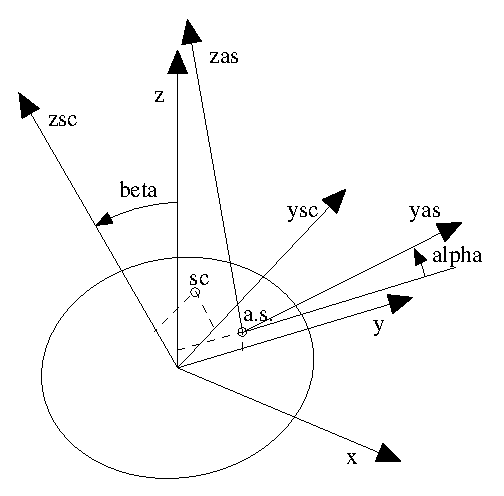
\includegraphics[width=.7\textwidth]{beamsect}
\caption{Beam section}
\label{fig:EL:BEAM:SECTION}
\end{figure}






\subsubsection{Generic Anisotropic Beam Section}
When a generic anisotropic beam section is considered,
the partitioning of axial and shear constitutive properties
of Figure~\ref{fig:EL:BEAM:GROUPS} is no longer possible.
The axial and shear straining can be completely and arbitrarily coupled,
resulting in a full constitutive matrix of the beam section,
\begin{align}
	\cubr{\cvvect{
		\T{f} \\
		\T{m}
	}}^\dagger
	&=
	\sqbr{\matr{cc}{
		\TT{K}_{\T{f}\T{\nu}} & \TT{K}_{\T{f}\T{\kappa}} \\
		\TT{K}_{\T{m}\T{\nu}} & \TT{K}_{\T{m}\T{\kappa}}
	}}^\dagger
	\cubr{\cvvect{
		\T{\nu} \\
		\T{\kappa}
	}}^\dagger ,
\end{align}
where $\T{f}$ and $\T{m}$ are the internal force and moment vectors,
while $\T{\nu}$ and $\T{\kappa}$ are the linear and angular strains.
Usually, $\TT{K}_{\T{m}\T{\nu}}\equiv\TT{K}_{\T{f}\T{\kappa}}^T$,
while $\TT{K}_{\T{f}\T{\nu}}$ and $\TT{K}_{\T{m}\T{\kappa}}$ are symmetric.


The reference point or the reference orientation of the constitutive
matrix can be changed by a sequence of transformations consisting
in a rotation and an offset.

The internal force and moment, after a rotation defined by the rotation
matrix $\TT{R}$, become
\begin{align}
	\cubr{\cvvect{
		\T{f} \\
		\T{m}
	}}^*
	&= \sqbr{\matr{cc}{
		\TT{R} & \TT{0} \\
		\TT{0} & \TT{R}
	}}
	\cubr{\cvvect{
		\T{f} \\
		\T{m}
	}}^\dagger
	.
\end{align}
Similarly, the strains become
\begin{align}
	\cubr{\cvvect{
		\T{\nu} \\
		\T{\kappa}
	}}^*
	&= \sqbr{\matr{cc}{
		\TT{R} & \TT{0} \\
		\TT{0} & \TT{R}
	}}^{-T}
	\cubr{\cvvect{
		\T{\nu} \\
		\T{\kappa}
	}}^\dagger
	\nonumber \\
	&= \sqbr{\matr{cc}{
		\TT{R} & \TT{0} \\
		\TT{0} & \TT{R}
	}}
	\cubr{\cvvect{
		\T{\nu} \\
		\T{\kappa}
	}}^\dagger
	.
\end{align}
As a consequence, the re-oriented constitutive relationship is
\begin{align}
	\cubr{\cvvect{
		\T{f} \\
		\T{m}
	}}^*
	&=
	\sqbr{\matr{cc}{
		\TT{R} & \TT{0} \\
		\TT{0} & \TT{R}
	}}
	\sqbr{\matr{cc}{
		\TT{K}_{\T{f}\T{\nu}} & \TT{K}_{\T{f}\T{\kappa}} \\
		\TT{K}_{\T{m}\T{\nu}} & \TT{K}_{\T{m}\T{\kappa}}
	}}^\dagger
	\sqbr{\matr{cc}{
		\TT{R} & \TT{0} \\
		\TT{0} & \TT{R}
	}}^T
	\cubr{\cvvect{
		\T{\nu} \\
		\T{\kappa}
	}}^*
	\nonumber \\
	&=
	\sqbr{\matr{cc}{
		\TT{R} \TT{K}_{\T{f}\T{\nu}}^\dagger \TT{R}^T
			& \TT{R} \TT{K}_{\T{f}\T{\kappa}}^\dagger \TT{R}^T \\
		\TT{R} \TT{K}_{\T{m}\T{\nu}}^\dagger \TT{R}^T
			& \TT{R} \TT{K}_{\T{m}\T{\kappa}}^\dagger \TT{R}^T
	}}
	\cubr{\cvvect{
		\T{\nu} \\
		\T{\kappa}
	}}^*
	\nonumber \\
	&=
	\sqbr{\matr{cc}{
		\TT{K}_{\T{f}\T{\nu}} & \TT{K}_{\T{f}\T{\kappa}} \\
		\TT{K}_{\T{m}\T{\nu}} & \TT{K}_{\T{m}\T{\kappa}}
	}}^*
	\cubr{\cvvect{
		\T{\nu} \\
		\T{\kappa}
	}}^*
	.
\end{align}

The internal moment, after considering an offset $\T{o}=\sqbr{0, y, z}^T$
of the reference point of the constitutive properties, becomes
$\T{m}=\T{m}^* + \T{o}\times\T{f}^*$.
The internal force and moment then becomes
\begin{align}
	\cubr{\cvvect{
		\T{f} \\
		\T{m}
	}}
	&= \sqbr{\matr{cc}{
		\TT{I} & \TT{0} \\
		\T{o}\times{} & \TT{I}
	}}
	\cubr{\cvvect{
		\T{f} \\
		\T{m}
	}}^*
	\label{eq:EL:BEAM:ANISOTROPIC-T}
	.
\end{align}
Similarly, the linear and angular strain vectors become
\begin{align}
	\cubr{\cvvect{
		\T{\nu} \\
		\T{\kappa}
	}}
	&= \sqbr{\matr{cc}{
		\TT{I} & \TT{0} \\
		\T{o}\times{} & \TT{I}
	}}^{-T}
	\cubr{\cvvect{
		\T{\nu} \\
		\T{\kappa}
	}}^*
	.
\end{align}
As a consequence, the offset constitutive relationship becomes
\begin{align}
	\cubr{\cvvect{
		\T{f} \\
		\T{m}
	}}
	&=
	\sqbr{\matr{cc}{
		\TT{I} & \TT{0} \\
		\T{o}\times{} & \TT{I}
	}}
	\sqbr{\matr{cc}{
		\TT{K}_{\T{f}\T{\nu}} & \TT{K}_{\T{f}\T{\kappa}} \\
		\TT{K}_{\T{m}\T{\nu}} & \TT{K}_{\T{m}\T{\kappa}}
	}}^*
	\sqbr{\matr{cc}{
		\TT{I} & \T{o}\times{}^T \\
		\TT{0} & \TT{I}
	}}
	\cubr{\cvvect{
		\T{\nu} \\
		\T{\kappa}
	}}
	\nonumber \\
	&=
	\sqbr{\matr{cc}{
		\TT{K}_{\T{f}\T{\nu}}^*
		& \TT{K}_{\T{f}\T{\nu}}^* \T{o}\times{}^T
			+ \TT{K}_{\T{f}\T{\kappa}}^* \\
		\T{o}\times\TT{K}_{\T{f}\T{\nu}}^*
			+ \TT{K}_{\T{m}\T{\nu}}^*
		& \T{o}\times\TT{K}_{\T{f}\T{\nu}}^* \T{o}\times{}^T
			+ \TT{K}_{\T{m}\T{\nu}}^* \T{o}\times{}^T
			+ \T{o}\times\TT{K}_{\T{f}\T{\kappa}}^*
			+ \TT{K}_{\T{m}\T{\kappa}}^*
	}}
	\cubr{\cvvect{
		\T{\nu} \\
		\T{\kappa}
	}}
	\nonumber \\
	&=
	\sqbr{\matr{cc}{
		\TT{K}_{\T{f}\T{\nu}} & \TT{K}_{\T{f}\T{\kappa}} \\
		\TT{K}_{\T{m}\T{\nu}} & \TT{K}_{\T{m}\T{\kappa}}
	}}
	\cubr{\cvvect{
		\T{\nu} \\
		\T{\kappa}
	}}^*
	.
\end{align}

It might be tempting to find what offset and rotation allows
to decouple the force and moment constitutive properties.
This can be sought by defining a generic transformation
\begin{align}
	\cubr{\cvvect{
		\T{f} \\
		\T{m}
	}}
	&= \sqbr{\matr{cc}{
		\TT{I} & \TT{0} \\
		\TT{T} & \TT{I}
	}}
	\cubr{\cvvect{
		\T{f} \\
		\T{m}
	}}^\dagger
	,
\end{align}
such that
\begin{align}
	\cubr{\cvvect{
		\T{f} \\
		\T{m}
	}}
	&=
	\sqbr{\matr{cc}{
		\TT{I} & \TT{0} \\
		\TT{T} & \TT{I}
	}}
	\sqbr{\matr{cc}{
		\TT{K}_{\T{f}\T{\nu}} & \TT{K}_{\T{f}\T{\kappa}} \\
		\TT{K}_{\T{m}\T{\nu}} & \TT{K}_{\T{m}\T{\kappa}}
	}}^\dagger
	\sqbr{\matr{cc}{
		\TT{I} & \TT{T}^T \\
		\TT{0} & \TT{I}
	}}
	\cubr{\cvvect{
		\T{\nu} \\
		\T{\kappa}
	}}
	\nonumber \\
	&=
	\sqbr{\matr{cc}{
		\TT{K}_{\T{f}\T{\nu}}^\dagger
		& \TT{K}_{\T{f}\T{\nu}}^\dagger \TT{T}^T
			+ \TT{K}_{\T{f}\T{\kappa}}^\dagger \\
		\TT{T}\TT{K}_{\T{f}\T{\nu}}^\dagger
			+ \TT{K}_{\T{m}\T{\nu}}^\dagger
		& \TT{T}\TT{K}_{\T{f}\T{\nu}}^\dagger \TT{T}^T
			+ \TT{K}_{\T{m}\T{\nu}}^\dagger \TT{T}^T
			+ \TT{T}\TT{K}_{\T{f}\T{\kappa}}^\dagger
			+ \TT{K}_{\T{m}\T{\kappa}}^\dagger
	}}
	\cubr{\cvvect{
		\T{\nu} \\
		\T{\kappa}
	}}
	.
\end{align}
The expected decoupling results from
\begin{align}
	\TT{T}
	&= 
	- \TT{K}_{\T{m}\T{\nu}}^\dagger
		\plbr{\TT{K}_{\T{f}\T{\nu}}^\dagger}^{-1}
	.
\end{align}
However, the resulting transformation $\TT{T}$ is not guaranteed
to have the skew-symmetric structure of $\T{o}\times{}$,
thus the decoupling may not be reducible to an offset.

The reverse transformation is relatively straightforward, after noticing
that, according to Eq.~(\ref{eq:EL:BEAM:ANISOTROPIC-T}), 
\begin{align}
	\cubr{\cvvect{
		\T{f} \\
		\T{m}
	}}^*
	&= \sqbr{\matr{cc}{
		\TT{I} & \TT{0} \\
		\T{o}\times{} & \TT{I}
	}}^{-1}
	\cubr{\cvvect{
		\T{f} \\
		\T{m}
	}}
	\nonumber \\
	&= \sqbr{\matr{cc}{
		\TT{I} & \TT{0} \\
		-\T{o}\times{} & \TT{I}
	}}
	\cubr{\cvvect{
		\T{f} \\
		\T{m}
	}}
	.
\end{align}
So, as expected, it is sufficient to revert the sign of the offset
to revert the transformation.
The signs of the constitutive relationship change accordingly.


\subsubsection{Locking Correction for Two-Node Beam}
The three-node finite volume element has been implemented first, 
and uses conventional polynomial parabolic interpolation 
of the nodal displacements and orientations;
the two-node finite volume element has been introduced later.
This latter element presents some shear-locking, which, for linear elastic
constitutive laws, may be overcome by correcting the section stiffness matrix
in a relatively straightforward form:
\begin{equation}\label{eq:2-NODE-BEAM-STIFFNESS}
	\hat{\T{K}} = \plbr{\T{F} + \frac{L^2}{12}\T{T} \T{F} \T{T}^T}^{-1} ,
\end{equation}
where $\T{F}=\T{K}^{-1}$ is the compliance matrix of the section, 
$L$ is the length of the beam, i.e.\ the distance between
the two reference points obtained by adding the optional offset 
to the nodes, and
\begin{displaymath}
	\T{T} \ = \ \sqbr{\matr{cc}{
		\T{0} & \T{e}_x \times{} \\
		\T{0} & \T{0}
	}}
\end{displaymath}
is the ``arm'' matrix that appears in the differential equilibrium equation
\begin{displaymath}
	\T{\vartheta}_{/x} - \T{T}^T\T{\vartheta} + \T{\phi} = 0
	,
\end{displaymath}
where $\T{\vartheta}=\sqbr{\T{f}^T \T{m}^T}^T$ are the internal forces
and moments, while $\T{\phi}$ are the external forces and moments
per unit span.

There are no provisions to automatically apply the correction 
when defining the constitutive law of the section.
The two-node beam has been reimplemented using a helicoidal interpolation
of the nodal positions and orientations, to improve its capability
to undergo large displacements and relative rotations.
It is activated by using the keyword \kw{hbeam2} instead of \kw{beam2}.
However, to reduce the shear-locking effect, the stiffness properties 
still need to be manually corrected according
to Equation~(\ref{eq:2-NODE-BEAM-STIFFNESS}).
The \kw{hbeam2} element is \emph{experimental}, and should be used
only for development purposes.


\subsection{Three-node beam element}
\label{sec:EL:BEAM:BEAM3}
The three-node beam element is described in detail in \cite{FV-AIAA}.
Each of the three points the beam element connects is referred
to a structural node but can have an arbitrary offset
to allow high generality in locating the structural reference line
of the beam.
Figure~\ref{fig:EL:BEAM:beam3} illustrates the geometry
of the three-node beam element.

\begin{figure}
\centering
\psfrag{1}{1}
\psfrag{2}{2}
\psfrag{3}{3}
\psfrag{n1}{node 1}
\psfrag{n2}{node 2}
\psfrag{n3}{node 3}
\psfrag{pI}{point I}
\psfrag{pII}{point II}
\psfrag{o1}{$\T{o}_1$}
\psfrag{o2}{$\T{o}_2$}
\psfrag{o3}{$\T{o}_3$}
\psfrag{RI}{$\TT{R}_I$}
\psfrag{RII}{$\TT{R}_{II}$}
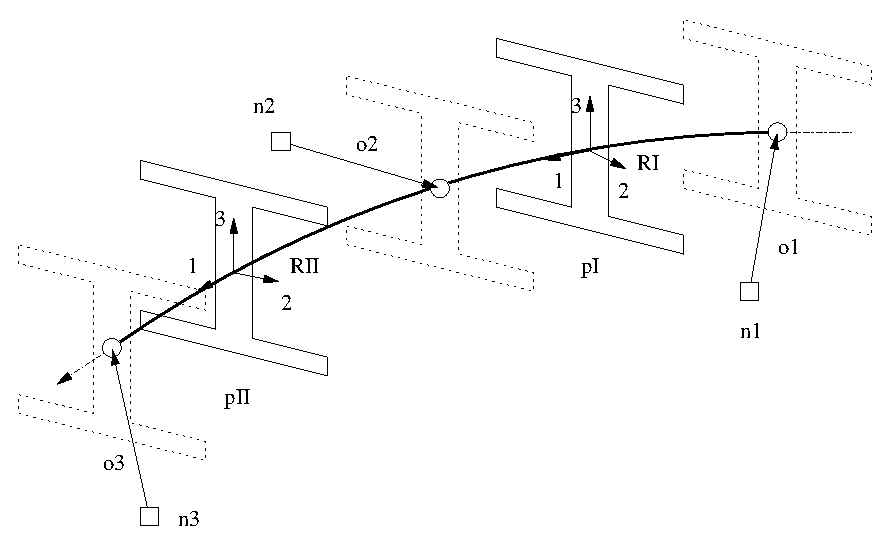
\includegraphics[width=.7\textwidth]{beam3}
\caption{Geometry of the three-node beam element.}
\label{fig:EL:BEAM:beam3}
\end{figure}

The finite volume formulation presented in \cite{FV-AIAA} is used.
As a consequence, the internal forces and moments are evaluated 
at two points that are at about midpoint between nodes 1 and 2, 
and nodes 2 and 3 (at $ \xi=-1/\sqrt{3}\cong -0.57735 $
and $\xi=1/\sqrt{3} \cong 0.57735$ of a non-dimensional abscissa $\xi$
running from $\xi=-1$ at node 1 to $\xi=1$ at node 3).

So the constitutive properties must be supplied in these points, as well as
the orientation matrices $\TT{R}_I$ and $\TT{R}_{II}$,
that express the orientation of the reference system
the constitutive properties are expressed in with respect to the global frame
(the axial force is conventionally defined in direction 1).
Any of the supported 6D constitutive laws can be supplied to define the
constitutive properties of each beam section.

The traditional input format is
%\begin{verbatim}
\begin{Verbatim}[commandchars=\\\{\}]
    \bnt{elem_type} ::= \kw{beam3}

    \bnt{normal_arglist} ::=
        \bnt{node_1_label} , (\ty{Vec3}) \bnt{relative_offset_1} ,
        \bnt{node_2_label} , (\ty{Vec3}) \bnt{relative_offset_2} ,
        \bnt{node_3_label} , (\ty{Vec3}) \bnt{relative_offset_3} ,
        (\ty{OrientationMatrix}) \bnt{orientation_matrix_section_I} ,
        (\ty{ConstitutiveLaw<6D>}) \bnt{constitutive_law_section_I} ,
        \{ \kw{same} | (\ty{OrientationMatrix}) \bnt{orientation_matrix_section_II} \} ,
        \{ \kw{same} | (\ty{ConstitutiveLaw<6D>}) \bnt{constitutive_law_section_II} \}
        [ , \bnt{custom_output} ]
\end{Verbatim}
%\end{verbatim}

The \nt{relative\_offset\_}\bnt{i}, with \nt{i}=1,2,3, are the vectors
$\T{o}_i$, with $i$=1,2,3, of Figure~\ref{fig:EL:BEAM:beam3}.

The orientation matrices \nt{orientation\_matrix\_section\_}\bnt{j},
with \nt{j}=I,II, are the section orientation matrices
$\TT{R}_j$, with $j$=$I$,$II$, of Figure~\ref{fig:EL:BEAM:beam3}.

The first keyword \kw{same}, alternative to the 
\nt{orientation\_matrix\_section\_II}, means that the same orientation
defined for the first point will be used for the second point.

The second keyword \kw{same}, alternative to the
\nt{constitutive\_law\_section\_II}, means that the same constitutive law
defined for the first point will be used for the second point.

If any of the constitutive laws is either viscous or viscoelastic,
the viscoelastic variant of the beam element is used.
Otherwise, the elastic variant is used.

A more complete input format is
%\begin{verbatim}
\begin{Verbatim}[commandchars=\\\{\}]
    \bnt{elem_type} ::= \kw{beam3}

    \bnt{normal_arglist} ::=
        \bnt{node_1_label} ,
            [ \kw{position} , ] (\ty{Vec3}) \bnt{relative_offset_1} ,
            [ \kw{orientation} , (\ty{OrientationMatrix}) \bnt{relative_orientation_1} , ]
        \bnt{node_2_label} ,
            [ \kw{position} , ] (\ty{Vec3}) \bnt{relative_offset_2} ,
            [ \kw{orientation} , (\ty{OrientationMatrix}) \bnt{relative_orientation_2} , ]
        \bnt{node_3} ,
            [ \kw{position} , ] (\ty{Vec3}) \bnt{relative_offset_3} ,
            [ \kw{orientation} , (\ty{OrientationMatrix}) \bnt{relative_orientation_3} , ]
        \{ (\ty{OrientationMatrix}) \bnt{orientation_matrix_section_I}
            | \kw{from nodes} \} ,
        (\ty{ConstitutiveLaw<6D>}) \bnt{constitutive_law_section_I} ,
        \{ \kw{same}
            | (\ty{OrientationMatrix}) \bnt{orientation_matrix_section_II}
            | \kw{from nodes} \} ,
        \{ \kw{same}
            | (\ty{ConstitutiveLaw<6D>}) \bnt{constitutive_law_section_II} \}
        [ , \bnt{custom_output} ]
\end{Verbatim}
%\end{verbatim}
This format is a superset of the traditional one, which is extended
by adding the possibility to set relative node orientations
that can be subsequently used to interpolate the orientation matrices
at the evaluation points, by providing the keyword \kw{from nodes}
instead of the matrix.
If the keyword \kw{same} is used for the second evaluation point,
the same method is used to compute the orientation matrix.

The \kw{custom\_output} optional data consists in
%\begin{verbatim}
\begin{Verbatim}[commandchars=\\\{\}]
    \bnt{custom_output} ::= \kw{custom output} , \bnt{custom_output_flag} [ , ... ]
\end{Verbatim}
%\end{verbatim}
The values of \nt{custom\_output\_flag}
are defined in Section~\ref{sec:CONTROLDATA:DEFAULTBEAMOUTPUT}.

Flags add up to form the custom output request.
Flags may not be repeated.
Strain rates are only available from viscoelastic beams.
By default, only forces are output, to preserve compatibility
with the original output format.
The custom output is only available in NetCDF format;
see Section~\ref{sec:NetCDF:Elem:Beam}.

As an example, a simple beam element, with diagonal section stiffness 
matrix is presented:
\begin{verbatim}
    set: integer beam_label = 1000;
    set: integer beam_node1 = 2001;
    set: integer beam_node2 = 2002;
    set: integer beam_node3 = 2003;
    set: real EA = 1e6;   # N
    set: real GAy = .6e6; # N
    set: real GAy = .6e6; # N
    set: real GJ = 1.e3;  # Nm^2
    set: real EJy = 2.e3; # Nm^2
    set: real EJz = 1.e4; # Nm^2
    beam3: beam_label,
        beam_node1, reference, node, null,
        beam_node2, reference, node, null,
        beam_node3, reference, node, null,
        eye,
        linear elastic generic, diag,
            EA, GAy, GAz, GJ, EJy, EJz,
        same,
        same;
\end{verbatim}

A not-so-simple beam section, where the center of axial strain 
and the shear center are not coincident, is illustrated below.
The node offset is used to align the reference line 
with the shear center, and the axial strain center offset 
is used in the constitutive matrix:
\begin{verbatim}
    set: integer beam_label = 1000;
    set: integer beam_node1 = 2001;
    set: integer beam_node2 = 2002;
    set: integer beam_node3 = 2003;
    set: real EA = 1e6;    # N
    set: real GAy = .6e6;  # N
    set: real GAy = .6e6;  # N
    set: real GJ = 1.e3;   # Nm^2
    set: real EJy = 2.e3;  # Nm^2
    set: real EJz = 1.e4;  # Nm^2
    set: real yas = 2.e-2; # m
    set: real zas = 1.e-2; # m
    set: real ysc = 4.e-2; # m
    set: real zsc = 2.e-2; # m
    set: real y = yas-ysc; # compute the axial strain center
    set: real z = zas-zsc; # wrt/ the shear center
    beam3: beam_label,
        beam_node1, reference, node, 0.,ysc,zsc,
        beam_node2, reference, node, 0.,ysc,zsc,
        beam_node3, reference, node, 0.,ysc,zsc,
        eye,
        linear elastic generic, sym,
            EA, 0.,  0.,  0., z*EA,       -y*EA,
                GAy, 0.,  0., 0.,          0.,
                     GAz, 0., 0.,          0.,
                          GJ, 0.,          0.,
                              EJy+z^2*EA, -z*y*EA,
                                           EJz+y^2*EA,
        same,
        same;
\end{verbatim}


A piezoelectric actuator beam element is available; an arbitrary
linear piezoelectric actuation matrix is required, together with the labels
of the abstract nodes that represent the input signal tensions, as follows:
%\begin{verbatim}
\begin{Verbatim}[commandchars=\\\{\}]
    \bnt{normal_arglist} ::=
        \bnt{node_1_label} , (\ty{Vec3}) \bnt{relative_offset_1} ,
        \bnt{node_2_label} , (\ty{Vec3}) \bnt{relative_offset_2} ,
        \bnt{node_3_label} , (\ty{Vec3}) \bnt{relative_offset_3} ,
        (\ty{OrientationMatrix}) \bnt{orientation_matrix_section_I} ,
        (\ty{ConstitutiveLaw<6D>}) \bnt{constitutive_law_section_I} ,
        \{ \kw{same} | (\ty{OrientationMatrix}) \bnt{orientation_matrix_section_II} \} ,
        \{ \kw{same} | (\ty{ConstitutiveLaw<6D>}) \bnt{constitutive_law_section_II} \} ,
        \kw{piezoelectric actuator} , 
            \bnt{electrodes_number} ,
            \bnt{abstract_node_label_list} ,
            (\ty{Mat6xN}) \bnt{piezoelectric_matrix_I} ,
            \{ \kw{same} | (\ty{Mat6xN}) \bnt{piezoelectric_matrix_II} \}
        [ , \bnt{custom_output} ]
\end{Verbatim}
%\end{verbatim}
where the \nt{abstract\_node\_label\_list} is the list of the labels of the
abstract nodes that represent the electrodes.


\paragraph{Private Data}
\label{sec:EL:BEAM:PRIVATE}
The following data is available:
\begin{enumerate}
\item \kw{"ex"} axial strain
\item \kw{"ey"} shear strain (local axis 2)
\item \kw{"ez"} shear strain (local axis 3)
\item \kw{"kx"} curvature about local axis 1 (torsional)
\item \kw{"ky"} curvature about local axis 2 (bending)
\item \kw{"kz"} curvature about local axis 3 (bending)
\item \kw{"Fx"} axial force
\item \kw{"Fy"} shear force (direction 2)
\item \kw{"Fz"} shear force (direction 3)
\item \kw{"Mx"} moment about local axis 1 (torsional)
\item \kw{"My"} moment about local axis 2 (bending)
\item \kw{"Mz"} moment about local axis 3 (bending)
\item \kw{"Xx"} absolute position component 1
\item \kw{"Xy"} absolute position component 2
\item \kw{"Xz"} absolute position component 3
\item \kw{"Phix"} absolute orientation vector component 1
\item \kw{"Phiy"} absolute orientation vector component 2
\item \kw{"Phiz"} absolute orientation vector component 3
\item \kw{"Omegax"} absolute angular velocity component 1
\item \kw{"Omegay"} absolute angular velocity component 2
\item \kw{"Omegaz"} absolute angular velocity component 3
\item \kw{"ePx"} axial strain rate
\item \kw{"ePy"} shear strain rate (local axis 2)
\item \kw{"ePz"} shear strain rate (local axis 3)
\item \kw{"kPx"} curvature rate about local axis 1 (torsional)
\item \kw{"kPy"} curvature rate about local axis 2 (bending)
\item \kw{"kPz"} curvature rate about local axis 3 (bending)
\end{enumerate}
Each string is prefixed by \kw{"pI."} or \kw{"pII."}
to specify data related to either the first or the second point:
\begin{verbatim}
    "pI.Fx"     # axial force at point I
    "pII.kz"    # bending curvature about local axis 3 at point II
\end{verbatim}
Private data related to point I are numbered from 1 to 27;
private data related to point II are numbered from 28 to 54.








\subsection{Two-node beam element}
\label{sec:EL:BEAM:BEAM2}
Similar considerations apply to the two-node beam.
Its geometry is illustrated in Figure~\ref{fig:EL:BEAM:beam2}.

\begin{figure}
\centering
\psfrag{1}{1}
\psfrag{2}{2}
\psfrag{3}{3}
\psfrag{n1}{node 1}
\psfrag{n2}{node 2}
\psfrag{pI}{point I}
\psfrag{o1}{$\T{o}_1$}
\psfrag{o2}{$\T{o}_2$}
\psfrag{RI}{$\TT{R}_I$}
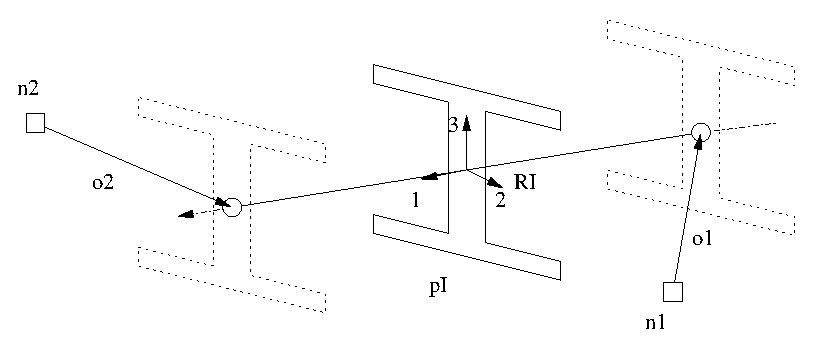
\includegraphics[width=.7\textwidth]{beam2}
\caption{Geometry of the two-node beam element.}
\label{fig:EL:BEAM:beam2}
\end{figure}

The syntax is
%\begin{verbatim}
\begin{Verbatim}[commandchars=\\\{\}]
    \bnt{elem_type} ::= \kw{beam2}

    \bnt{normal_arglist} ::=
        \bnt{node_1_label} , (\ty{Vec3}) \bnt{relative_offset_1} ,
        \bnt{node_2_label} , (\ty{Vec3}) \bnt{relative_offset_2} ,
        (\ty{OrientationMatrix}) \bnt{orientation_matrix_section_I} ,
        (\ty{ConstitutiveLaw<6D>}) \bnt{constitutive_law_section_I}
        [ , \kw{piezoelectric actuator} , 
            \bnt{electrodes_number} ,
            \bnt{abstract_node_label_list} ,
            (\ty{Mat6xN}) \bnt{piezoelectric_matrix_I} ]
        [ , \bnt{custom_output} ]
\end{Verbatim}
%\end{verbatim}

A more complete form is
%\begin{verbatim}
\begin{Verbatim}[commandchars=\\\{\}]
    \bnt{elem_type} ::= \kw{beam2}

    \bnt{normal_arglist} ::=
        \bnt{node_1_label} ,
            [ \kw{position} , ] (\ty{Vec3}) \bnt{relative_offset_1} ,
            [ \kw{orientation} , (\ty{OrientationMatrix}) \bnt{relative_orientation_1} , ]
        \bnt{node_2_label} ,
            [ \kw{position} , ] (\ty{Vec3}) \bnt{relative_offset_2} ,
            [ \kw{orientation} , (\ty{OrientationMatrix}) \bnt{relative_orientation_2} , ]
        \{ (\ty{OrientationMatrix}) \bnt{orientation_matrix_section_I}
            | \kw{from nodes} \} ,
        (\ty{ConstitutiveLaw<6D>}) \bnt{constitutive_law_section_I}
        [ , \kw{piezoelectric actuator} , 
            \bnt{electrodes_number} ,
            \bnt{abstract_node_label_list} ,
            (\ty{Mat6xN}) \bnt{piezoelectric_matrix_I} ]
        [ , \bnt{custom_output} ]
\end{Verbatim}
%\end{verbatim}

\paragraph{Private Data.}
The same private data indicated for the \kw{beam3} element is available
(see Section~\ref{sec:EL:BEAM:PRIVATE}).
No prefix must be specified (\kw{"pI."} is implicit).


\paragraph{Example.} \
As an example, a simple beam element, with diagonal section stiffness 
matrix is presented:
\begin{verbatim}
    set: integer beam_label = 1000;
    set: integer beam_node1 = 2001;
    set: integer beam_node2 = 2002;
    set: real L = .4;     # m
    set: real EA = 1e6;   # N
    set: real GAy = .6e6; # N
    set: real GAy = .6e6; # N
    set: real GJ = 1.e3;  # Nm^2
    set: real EJy = 2.e3; # Nm^2
    set: real EJz = 1.e4; # Nm^2
    beam2: beam_label,
        beam_node1, reference, node, null,
        beam_node2, reference, node, null,
        eye,
        linear elastic generic, diag,
            EA, 1./(1./GAy+L^2/12./EJz), 1./(1./GAz+L^2/12./EJy),
            GJ, EJy, EJz;
\end{verbatim}
Note that the shear terms have been na\"{\i}vely inverted to eliminate
shear locking, according to Equation~(\ref{eq:2-NODE-BEAM-STIFFNESS}).



\subsection{Output}
The output related to beam elements is contained in a file with extension 
\texttt{.act}; for each time step, the output of the required beams is
written.
The internal forces and couples are computed from the interpolated strains
along the beam by means of the constitutive law, at the two evaluation
points. 
The format is:
\begin{itemize}
    \item the label of the beam
    \item the three components of the force at the first evaluation point
    \item the three components of the couple at the first evaluation point
    \item the three components of the force at the second evaluation point
    \item the three components of the couple at the second evaluation point    
\end{itemize}
The last two items (i.e.\ the last 6 columns) are generated
only by the three-node beam element.

More detailed output is allowed when using NetCDF;
see Section~\ref{sec:NetCDF:Elem:Beam} for details.



\subsection{Notes}
Two-node beam elements should be used with care.



\section{Body}
%\begin{verbatim}
\begin{Verbatim}[commandchars=\\\{\}]
    \bnt{elem_type} ::= \kw{body}

    \bnt{normal_arglist} ::= \bnt{node_label} ,
        \{ \bnt{one_body}
            | \kw{condense} , \bnt{num_masses} , \bnt{one_body} [ , ... ] \}

    \bnt{one_body} ::=
        (\ty{Scalar}) \bnt{mass} , 
        (\ty{Vec3})   \bnt{relative_center_of_mass} ,
        (\ty{Mat3x3}) \bnt{inertia_matrix}
        [ , \kw{inertial} , 
            \{ \kw{node} | (\ty{OrientationMatrix}) \bnt{orientation_matrix} \} ]
\end{Verbatim}
%\end{verbatim}
If only one mass is defined, the first method should be used. Otherwise,
many masses can be referred to the same element by means of the keyword
\kw{condense}, followed by the number of expected masses \nt{num\_masses}.
The format of each sub-mass is the same as for the single mass input (actually, 
when \kw{condense} is not supplied, \nt{num\_masses} is assumed to be 1).

The \nt{inertia\_matrix} is always referred to the center of mass of the
mass that is being added. It can be rotated locally by means of the extra
\nt{orientation\_matrix} supplied after the (optional) keyword \kw{inertial}.
The keyword \kw{node} corresponds to the default, i.e.\ the inertia matrix
is assumed to be input in the node reference frame.

Note: in many commercial finite element software, the off-diagonal elements 
of the inertia matrix are defined with a minus sign; for instance, 
NASTRAN's \texttt{CONM2} lumped inertia card expects the values as indicated
in Figure~\ref{fig:el:body:CONM2}.
%
\begin{figure}[b]
\centering
\begin{minipage}{120mm}
\begin{boxedverbatim}
$.......2.......3.......4.......5.......6.......7.......8.......
CONM2   EID     G       CID     M       X1      X2      X3
        I11     I21     I22     I31     I32     I33
\end{boxedverbatim}
\end{minipage}
\caption{NASTRAN \texttt{CONM2} card}
\label{fig:el:body:CONM2}
\end{figure}
%
However, the matrix is reconstructed as
\begin{displaymath}
	\mathrm{NASTRAN \ ::= } \ \sqbr{\matr{rrrrrr}{
		\texttt{M} & & & & & \\
		& \texttt{M} & & \multicolumn{3}{c}{\text{symmetric}} \\
		& & \texttt{M} & & & \\
		& & & \texttt{I11} & & \\
		& & & -\texttt{I21} & \texttt{I22} & \\
		& & & -\texttt{I31} & -\texttt{I32} & \texttt{I33}
	}}
\end{displaymath}
see for instance \emph{NASTRAN V70.5 Quick Reference Guide} for details.

\noindent
On the contrary, MBDyn directly reads the matrix 
that will be used in the computation, i.e.\ 
\textbf{without the minus signs in the off-diagonal terms},
as reported below:
\begin{displaymath}
	\mathrm{MBDyn \ ::= } \ \sqbr{\matr{ccc}{
		\texttt{i11} & \texttt{i12} & \texttt{i13} \\
		& \texttt{i22} & \texttt{i23} \\
		\multicolumn{2}{l}{\text{sym.}} & \texttt{i33}
	}}
\end{displaymath}
So:
\begin{eqnarray*}
	\texttt{i11} & = & \texttt{I11} \\
	\texttt{i22} & = & \texttt{I22} \\
	\texttt{i33} & = & \texttt{I33} \\
	\texttt{i12} & = & - \texttt{I21} \\
	\texttt{i13} & = & - \texttt{I31} \\
	\texttt{i23} & = & - \texttt{I32}
\end{eqnarray*}
The inertia properties of the model can be logged and verified
by means of the \kw{inertia} keyword, as detailed
in Section~\ref{sec:EL:MISC:INERTIA}.

\paragraph{Example.} \
\begin{verbatim}
    set: integer NODE_LABEL = 100;
    set: integer BODY_LABEL = 100;

    # single mass example
    body: BODY_LABEL, NODE_LABEL,
        8.,                            # mass
        reference, node, 0., 0., 0.,   # c.m. offset
        diag, 4.8, 4.8, .4;            # inertia tensor

    # three masses example (equivalent to the previous one)
    body: BODY_LABEL, NODE_LABEL,
        condense, 3,
        4.,                            # mass 1 (mid)
        reference, node, 0., 0., 0.,   # c.m. offset 1
        diag, .4, .4, .2,              # inertia tensor 1
        2.,                            # mass 2 (top)
        reference, node, 0., 0., 1.,   # c.m. offset 2
        diag, .2, .2, .1,              # inertia tensor 2
        2.,                            # mass 3 (bottom)
        reference, node, 0., 0., -1.,  # c.m. offset 3
        diag, .2, .2, .1;              # inertia tensor 3
\end{verbatim}



\section{Bulk Elements}
The \kw{bulk} element is intended as a sort of NASTRAN's \texttt{CELAS} card,
that can be used to apply a stiffness term on an arbitrary degree of freedom.
Extensions are planned to different kind of elements.
The syntax of the \kw{bulk} element is:
%\begin{verbatim}
\begin{Verbatim}[commandchars=\\\{\}]
    \bnt{elem_type} ::= \kw{bulk}

    \bnt{normal_arglist} ::= \bnt{bulk_type} , \bnt{bulk_arglist}
\end{Verbatim}
%\end{verbatim}
At present only the \kw{stiffness spring} type is available.

\subsection{Stiffness spring}
%\begin{verbatim}
\begin{Verbatim}[commandchars=\\\{\}]
    \bnt{bulk_type} ::= \kw{stiffness spring}

    \bnt{bulk_arglist} ::=
        (\ty{NodeDof}) \bnt{dof} ,
        (\ty{DriveCaller}) \bnt{stiffness_drive}
\end{Verbatim}
%\end{verbatim}
The equation related to the desired dof of the linked node is added a
contribution based on the value of the desired degree of freedom (even the
derivative can be used) multiplied times the stiffness.

{\em Note: this family of elements has been partially superseded by the
\htmlref{\kw{genel}}{sec:EL:GENEL} elements, which allow more generality.}




\section{Couple}
A variant of \kw{force}; see Section~\ref{sec:EL:FORCE} for details.




\section{Electric Elements}
\kw{electric} elements are those elements that model electric and electronic
devices, dealing with abstract degrees of freedom more than with electric
ones (from the program's point of view they are exactly the same, the
difference is only semantic). The true electric elements, such resistors,
switches and so on, are classified as \kw{electric bulk} elements.
The syntax for \kw{electric} elements is:
%\begin{verbatim}
\begin{Verbatim}[commandchars=\\\{\}]
    \bnt{normal_arglist} ::= \bnt{electric_type} , \bnt{electric_arglist}
\end{Verbatim}
%\end{verbatim}
The \kw{electric} elements implemented at present are:
\begin{itemize}
	\item \kw{accelerometer}
	\item \kw{displacement}
	\item \kw{motor}
	\item \kw{discrete control}
\end{itemize}
The syntax is described in the following.

\subsection{Accelerometer}
%\begin{verbatim}
\begin{Verbatim}[commandchars=\\\{\}]
    \bnt{electric_type} ::= \kw{accelerometer}

    \bnt{electric_arglist} ::=
        \{ \kw{translational} | \kw{rotational} \} ,
        \bnt{struct_node_label} ,
        \bnt{abstract_node_label} ,
        ((\ty{Unit})\ty{Vec3}) \bnt{measure_direction}
        [ , \kw{position} , (\ty{Vec3}) \bnt{position} ]
\end{Verbatim}
%\end{verbatim}
The \kw{position} is optional; it is meaningless for \kw{rotational}
accelerometers.
The measure is taken along or about direction \nt{measure\_direction};
the vector is internally normalized to unity.

\noindent
Legacy element: accelerometer with built-in transfer function
%\begin{verbatim}
\begin{Verbatim}[commandchars=\\\{\}]
    \bnt{electric_type} ::= \kw{accelerometer}

    \bnt{electric_arglist} ::= \bnt{struct_node_label} ,
        \bnt{abstract_node_label} ,
        ((\ty{Unit})\ty{Vec3}) \bnt{measure_direction} ,
        (\ty{Scalar}) \bnt{omega} ,
        (\ty{Scalar}) \bnt{tau} ,
        (\ty{Scalar}) \bnt{csi} ,
        (\ty{Scalar}) \bnt{kappa}	
\end{Verbatim}
%\end{verbatim}
The label \nt{struct\_node\_label} defines the node whose acceleration 
is being measured; the label \nt{abstract\_node\_label} defines the
\kw{abstract node} that will receive the output signal. 
An \kw{electric node} can be used as well (?).
The measure is taken along direction \nt{measure\_direction};
the vector is internally normalized to unity.
The transfer function of the accelerometer is:
\begin{displaymath}
    \frac{e_0}{a} = \nt{kappa} \cdot \frac{\nt{tau} \cdot s}{
        \plbr{1 + \nt{tau} \cdot s}
        \plbr{1 + 2 \cdot \nt{csi} \cdot (s/\nt{omega}) + (s/\nt{omega})^2}
    }
\end{displaymath}
where $ e_0 $ is the output signal, $ a $ is the input (the acceleration)
and $ s $ is Laplace's variable.



\subsection{Displacement}
%\begin{verbatim}
\begin{Verbatim}[commandchars=\\\{\}]
    \bnt{electric_type} ::= \kw{displacement}

    \bnt{electric_arglist} ::=
        \bnt{struct_node_1_label} , (\ty{Vec3}) \bnt{relative_offset_1} ,
        \bnt{struct_node_2_label} , (\ty{Vec3}) \bnt{relative_offset_2} ,
        \bnt{abstract_node_label}
\end{Verbatim}
%\end{verbatim}
\begin{subequations}
\begin{align}
	\T{d} &= \T{x}_b + \T{o}_b - \T{x}_a - \T{o}_a \\
	x &= \sqrt{\T{d}^T \T{d}}
\end{align}
\end{subequations}
The value $x$ is added to the right-hand side of the equation
of the \kw{abstract} node.

\subsection{Motor}
%\begin{verbatim}
\begin{Verbatim}[commandchars=\\\{\}]
    \bnt{electric_type} ::= \kw{motor}

    \bnt{electric_arglist} ::=
        \bnt{struct_node_1_label} ,
        \bnt{struct_node_2_label} ,
        ((\ty{Unit})\ty{Vec3}) \bnt{direction_relative_to_node_1} ,
        \bnt{abstract_node_1_label} ,
        \bnt{abstract_node_2_label} ,
        (\ty{Scalar}) \bnt{dG},
        (\ty{Scalar}) \bnt{dL},
        (\ty{Scalar}) \bnt{dR}
\end{Verbatim}
%\end{verbatim}
\begin{subequations}
\begin{align}
	\omega &= \T{e}^T \plbr{\T{\omega}_2 - \T{\omega}_1} \\
	V &= V_2 - V_1 \\
	V &= \nt{dL} \frac{\mathrm{d}i}{\mathrm{d}t} + \nt{dR} \, i + \nt{dG} \, \omega \\
	\T{c}_1 &= - \T{e} \, \nt{dG} \, i \\
	\T{c}_2 &= \T{e} \, \nt{dG} \, i \\
	i_1 &= -i \\
	i_2 &= i
\end{align}
\end{subequations}
The motor applies an internal torque about direction
$\T{e}=\nt{direction\_relative\_to\_node\_1}$
to both the structural nodes it is connected to.
The direction $\T{e}$ is internally normalized to unity.
It also applies a current to both the electrical nodes it is connected to.

The element assumes that the relative orientation between nodes 1 and 2
can only change by rotating about direction $\T{e}$, so appropriate
joints must be in place.


\subsection{Discrete control}\label{sec:EL:DISCCTRL}
This element implements a discrete equation
that can be used to represent the behavior
of a discrete linear controller.
The control matrices can be either provided,
or identified during the simulation by recursive least squares.

Assume the original system consists in a generic nonlinear process
that depends on a set of measures $\T{y}$ and a set of inputs $\T{u}$
at a finite number of time steps past the current time, $t_k$, namely
\begin{align}
	\T{f}\plbr{\T{y}_{k - i}, \T{u}_{k - j}} = \T{0} ,
\end{align}
with $i=0,p$ and $j=0,q$.
Only $\T{y}_k$ is unknown, and thus represents the output of the process.
It is assumed that $\T{u}_k$ is known, and represents an input
to the process.

This element implements a controller of the form
\begin{align}
	\T{u}_{ck}
	&= \sum_{i=1,p} \TT{B}_{ci} \T{u}_{k - i}
	+ \sum_{j=1,q} \TT{A}_{cj} \T{y}_{k - j} ,
\end{align}
where $\T{u}_{ck}$ is the control input that must be applied
at time $t_k$ in addition to any exogenous input $\T{u}_{ek}$,
so that $\T{u}_k = \T{u}_{ek} + \T{u}_{ck}$.
The control input $\T{u}_{ck}$ can only depend on the measures
and the inputs at previous time steps.

Note that the symbols commonly used for discrete systems
are here reversed, since the element is intended to compute
the control signals at time $t_k$, $\T{u}_{ck}$,
based on the previous value of the controls,
$\T{u}_{k-i} = \T{u}_{e(k - i)} + \T{u}_{c(k - i)}$,
and on the previous value of the motion of the original system,
$\T{y}_{k-j}$;
$\T{u}_e$ indicates a generic measured exogenous input
to the system to be controlled.

The order $p$ and $q$ of the auto-regressive and exogenous portions
of the system can differ.
In detail, the order $p$ can be zero; in that case, the system
implements a \emph{finite impulse response} function.

This element is not self-starting; it assumes that both
inputs and outputs at times before the start time are zero.

The so-called ``output'' signals, indicated with $\T{y}$,
can be instances of either \ty{NodeDof} or \ty{DriveCaller} objects.
The so-called ``input'' signals, indicated with $\T{u}$,
must be instances of \ty{NodeDof} object.
This implies that instances of \ty{NodeDof} objects
need the corresponding equations to be (at least) statically defined.
In fact, the \kw{discrete control} element uses the ``output''
\ty{NodeDof} values, the $\T{y}$, to compute the corresponding
``inputs'', the $\T{u}$.
The latter are substantially added as a right-hand side
to the equations of the corresponding \ty{NodeDof} objects.
As a consequence, other elements must contribute to the left-hand side
of all the \ty{NodeDof} equations in order to make them defined.

Note that other elements may also contribute to the right-hand side
of the ``input'' \ty{NodeDof} object.
Specifically, other \kw{abstract} forces may contribute to their value.
In that case, the additional forces represent the exogenous inputs.
They are considered as part of the input used by the \kw{discrete control}
element, since the value $\T{u}_k$ to be used in the control equation
is extracted from the value of the corresponding \ty{NodeDof} objects.

Figure~\ref{fig:discctrl} illustrates the behavior of the element.
The typical suggested approach is illustrated later in an example.
\begin{figure}
\centering
\psfrag{A}{$\TT{A}$}
\psfrag{B}{$\TT{B}$}
\psfrag{f}{$\T{f}$}
\psfrag{uc}{$\T{u}_c$}
\psfrag{fe}{$\T{u}_e$}
\psfrag{uk-2}{$\T{u}_{k-2}$}
\psfrag{uk-1}{$\T{u}_{k-1}$}
\psfrag{uk}{$\T{u}_{k}$}
\psfrag{yk-2}{$\T{y}_{k-2}$}
\psfrag{yk-1}{$\T{y}_{k-1}$}
\psfrag{yk}{$\T{y}_{k}$}
\psfrag{k=1}{$\mathbb{K}=1$}
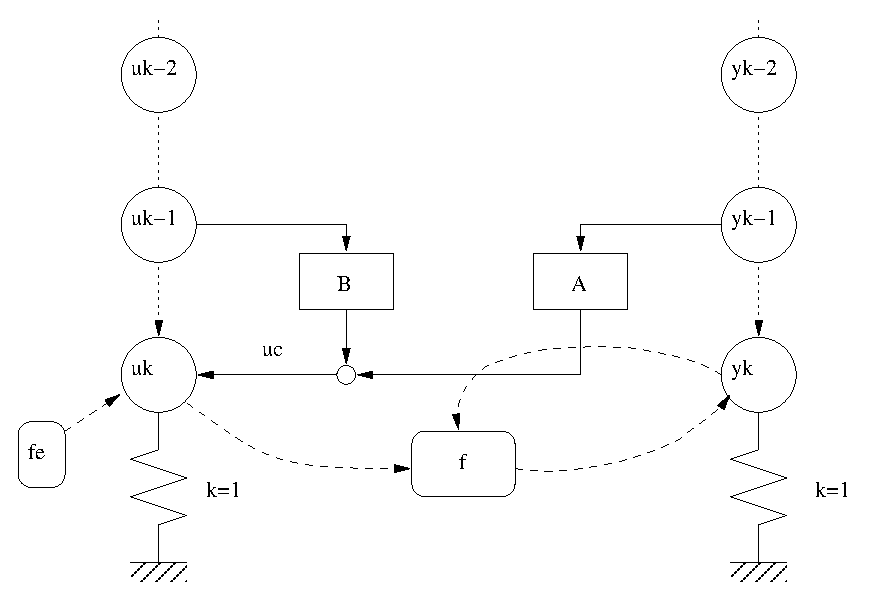
\includegraphics[width=.7\textwidth]{discctrl}
\caption{Discrete control layout.}
\label{fig:discctrl}
\end{figure}

The syntax is
%\begin{verbatim}
\begin{Verbatim}[commandchars=\\\{\}]
    \bnt{electric_type} ::= \kw{discrete control}

    \bnt{electric_arglist} ::= \bnt{num_outputs} , \bnt{num_inputs} ,
        \bnt{order_A} [ , \kw{fir} , \bnt{order_B} ] ,
        \bnt{num_iter} ,
        \bnt{control_data} , 
        \kw{outputs} ,
            (\ty{ScalarValue}) \bnt{output_value}
                [ , \kw{scale} , (\ty{DriveCaller}) \bnt{scale} ]
            [ , ... ] ,
        \kw{inputs} ,
            (\ty{NodeDof}) \bnt{input_dof}
            [ , ... ]

    \bnt{output_value} ::=
        \{ [ \kw{node dof} , ] (\ty{NodeDof}) \bnt{output_dof}
            | \kw{drive} , (\ty{DriveCaller}) \bnt{output_drive} \}
\end{Verbatim}
%\end{verbatim}
The lists of the output and input dofs follows. The inputs
do not require the \nt{order\_A} and \nt{order\_B} fields,
since they are simply used to compute the control forces,
and thus identify an equation.
\nt{order\_B} defaults to \nt{order\_A} unless a \kw{fir} control is chosen.

The \nt{control\_data} has the syntax:
%\begin{verbatim}  
\begin{Verbatim}[commandchars=\\\{\}]
        \bnt{control_data} ::= \bnt{control_type} , \bnt{control_arglist}
\end{Verbatim}
%\end{verbatim}
At present only a simple form of control is implemented. Other types
to come are system identification, both recursive and one-shot, and
adaptive control, with different models and schemes, all based on 
Generalized Predictive Control (GPC) and Deadbeat Control.
The \nt{control\_data} syntax is:
%\begin{verbatim}
\begin{Verbatim}[commandchars=\\\{\}]
    \bnt{control_data} ::=
        \{ \kw{control} , " \bnt{control_matrices_file} "
            | \kw{identification} , \bnt{identification_data}
            | \kw{adaptive control} , \bnt{adaptive_control_data} \}
\end{Verbatim}
%\end{verbatim}

\subsubsection{Control}
The file \nt{control\_matrices\_file} must contain the matrices
$ a_c $, $ b_c $ of the control in plain text (as generated by Matlab, for
instance):

\noindent
\begin{tabular}{l}
    $ a_{c1} $, \\
    \ldots,     \\
    $ a_{cp} $, \\
    $ b_{c1} $, \\
    \ldots,     \\
    $ b_{cp} $  \\
\end{tabular} \\
where $ p $ is the \nt{order\_A} of the controller and the matrices $ a_c $
have \nt{num\_inputs} rows and \nt{num\_outputs} columns, while the
matrices $ b_c $ have \nt{num\_inputs} rows and \nt{num\_inputs} columns.

\subsubsection{Identification}
%\begin{verbatim}
\begin{Verbatim}[commandchars=\\\{\}]
    \bnt{identification_data} ::=
        \{ \kw{arx} | \kw{armax} \}
        [ , \bnt{forgetting_factor} ]
        [ , \bnt{persistent_excitation} ]
        [ , \kw{file} , " \bnt{output_file_name} " ]
\end{Verbatim}
%\end{verbatim}
The forgetting factor is defined as
%\begin{verbatim}
\begin{Verbatim}[commandchars=\\\{\}]
    \bnt{forgetting_factor} ::=
        \kw{forgettingfactor} ,
          \{ \kw{const} , \bnt{d}
              | \kw{dynamic} , \bnt{n1} , \bnt{n2} , \bnt{rho} , \bnt{fact} , \bnt{kref} , \bnt{klim} \}
\end{Verbatim}
%\end{verbatim}
The default is a \kw{const} forgetting factor with $\nt{d}=1$.

The \nt{persistent\_excitation} is defined as
%\begin{verbatim}
\begin{Verbatim}[commandchars=\\\{\}]
    \bnt{persistent_excitation} ::=
        \kw{excitation} , (\ty{DriveCaller}) \bnt{excitation_drive} [ , ... ]
\end{Verbatim}
%\end{verbatim}
where \nt{num\_inputs} instances of \nt{excitation\_drive} must be defined.
By default, no persistent excitation is defined.

\subsubsection{Adaptive control}
The \nt{adaptive\_control\_data} card is
%\begin{verbatim}
\begin{Verbatim}[commandchars=\\\{\}]
    \bnt{adaptive_control_data} ::=
        [ \{ \kw{arx} | \kw{armax} \} , ]
        [ \kw{periodic} , \bnt{periodic_factor} , ]
        \{ \kw{gpc} ,
            \bnt{prediction_advancing_horizon} ,
            \bnt{control_advancing_horizon} ,
            \bnt{prediction_receding_horizon} ,
            [ \kw{prediction weights} , \bnt{Wi} [ , ... ] , ]
            [ \kw{control weights} , \bnt{Ri} [ , ... ] , ]
            (\ty{DriveCaller}) \bnt{weight_drive}
        | \kw{deadbeat} ,
            \bnt{prediction_advancing_horizon} ,
            \bnt{control_advancing_horizon} \}
        [ , \bnt{forgetting_factor} ]
        [ , \bnt{persistent_excitation} ]
        [ , \kw{trigger} , (\ty{DriveCaller}) \bnt{trigger_drive} ]
        [ , \kw{desired output} , (\ty{DriveCaller}) \bnt{output_drive} [ , ... ] ]
        [ , \kw{file} , " \bnt{file_name} " ]
\end{Verbatim}
%\end{verbatim}
The default is \kw{arx}.

The meaning of the keywords is:
\begin{itemize}
\item the \nt{periodic\_factor} defaults to 0;

\item if the keyword \kw{prediction weights} is present,
a number of weights \nt{Wi} equal to
\begin{quote}
$(\nt{prediction\_advancing\_horizon} - \nt{prediction\_receding\_horizon})$
\end{quote}
must be supplied.
If the keyword \kw{control weights} is present,
a number of weights \nt{Ri} equal to \nt{control\_advancing\_horizon}
must be supplied.
If the keywords are not defined, the corresponding weights
default to 1;

\item the \kw{desired output}
option requires \nt{num\_outputs} drives to be defined.
\end{itemize}

\subsubsection{Private Data}
The following data is available:
\begin{enumerate}
\item \kw{"u[\bnt{idx}]"} value of the \nt{idx}-th control output.
\end{enumerate}

\subsubsection{Examples}
Consider the case of a discrete controller that computes
a set of control signals $\T{u}_k$ by adding to their value
at the previous step, $\T{u}_{k-1}$, a contribution coming
from some measure $\T{y}_{k-1}$.
The control matrices are
\begin{subequations}
\begin{align}
	\TT{A}_{c1} &= \sqbr{\matr{cc}{
		a_{11} & a_{12} \\
		a_{21} & a_{22}
	}} \\
	\TT{B}_{c1} &= \sqbr{\matr{cc}{
		1 & 0 \\
		0 & 1
	}}
\end{align}
\end{subequations}
They are defined in the control data file \texttt{discretecontrol.dat} as
\begin{verbatim}
    a_11 a_12
    a_21 a_22
    1.0 0.0
    0.0 1.0
\end{verbatim}
The model consists in two abstract nodes for the control input
\ty{NodeDof} objects.
They need to be grounded.
This can be formulated by using a \kw{spring support} \kw{genel}
for each \kw{abstract} node, characterized by a unit spring coefficient,
such that
\begin{subequations}
\begin{align}
	1 \cdot x_{u1} = u_1 \\
	1 \cdot x_{u2} = u_2
\end{align}
\end{subequations}
Moreover, assume that the first measure, $y_1$,
comes from a \ty{NodeDof} object,
while the second one, $y_2$, comes from a \ty{DriveCaller} object.
The equation corresponding to $y_1$ must be appropriately grounded
as well, for example by means of yet another \kw{spring support}
\kw{genel}.
This is outside the scope of the present example, so it will assume
the output nodes are defined appropriately.

The model is
\begin{verbatim}
    set: integer U_1 = 1;
    set: integer U_2 = 2;
    set: integer Y_1 = 11;
    # ...
    abstract: U_1;
    abstract: U_2;
    # ...
    genel: U_1, spring support,
        U_1, abstract, algebraic,
        linear elastic, 1.;
    genel: U_2, spring support,
        U_2, abstract, algebraic,
        linear elastic, 1.;
    electric: 99, discrete control,
        2,    # number of `outputs' y
        2,    # number of `inputs' u
        1,    # order of output matrices A (same for input matrices B)
        1,    # update every iteration
        control, "discretecontrol.dat",
        outputs,
            node dof, Y_1, abstract, algebraic, scale, 1.e-3,
            drive, sine, .5, 2*pi, 1., forever, 0, scale, 1.e-3,
        inputs,
            U_1, abstract, algebraic,
            U_2, abstract, algebraic;
\end{verbatim}




\section{Force}\label{sec:EL:FORCE}
The \kw{force} element is a general means to introduce 
a right-hand side to the equations, i.e.\ an explicit contribution
to the equations.
There is a basic distinction between abstract and structural forces:
abstract forces apply to arbitrary equations, while structural forces
(and couples) are specific to structural nodes and have
a spatial characterization.
Essentially, structural forces have three components
that may depend on arbitrary parameters (usually the simulated time),
and a location in space.
Structural couples have three parameter-dependent components.
The syntax of the \kw{force} element is:
%\begin{verbatim}
\begin{Verbatim}[commandchars=\\\{\}]
    \bnt{elem_type} ::= \{ \kw{force} | \kw{couple} \}

    \bnt{normal_arglist} ::= \bnt{force_type} , \bnt{force_arglist}

    \bnt{force_type} ::=
        \{ \kw{abstract} [ \kw{internal} ]                             # \kw{force}
            | \{ \kw{absolute} | \kw{follower} \} [ \kw{internal} ]          # \kw{force}, \kw{couple}
            | \kw{modal}                                         # \kw{force}
            | \kw{external} \{ \kw{structural} | \kw{modal} \} [ \kw{mapping} ] \} # \kw{force}
\end{Verbatim}
%\end{verbatim}
The \kw{abstract} \nt{force\_type} applies to generic equations;

The \kw{structural} force type only applies to equilibrium equations
related to \kw{structural} nodes.
The \kw{couple} element can only be structural.
It is discussed in this section because of its input syntax commonality 
with the structural \kw{force} elements.

The \kw{modal} \nt{force\_type} applies to equations related
to a \kw{modal} element.

The \kw{external structural} and the \kw{external modal} types
are essentially used to provide an easy to use interface
for coupling with external software in a loose or tight manner.

\subsection{Output}
The output is discussed according to the types of forces. 
The label of the element is output first in all the cases.

\subsection{Abstract force}\label{sec:EL:FORCE:ABSTRACT}
%\begin{verbatim}
\begin{Verbatim}[commandchars=\\\{\}]
    \bnt{elem_type} ::= \kw{force}

    \bnt{force_type} ::= \kw{abstract}

    \bnt{force_arglist} ::=
        (\ty{NodeDof})     \bnt{dof} ,
        (\ty{DriveCaller}) \bnt{force_magnitude}
\end{Verbatim}
%\end{verbatim}
the \nt{dof} field is a normal \ty{NodeDof}; no \kw{order} is required
since the \kw{force} simply applies to the equation related to the node,
regardless of the order.

\subsubsection{Output}
The format is:
\begin{itemize}
    \item the label of the element;
    \item the label of the node\footnote{Since the \kw{abstract} force type
	can connect to \ty{NodeDof}, information provided here
	can be partial if the \ty{NodeDof} actually represents
	a component of a node with more than one degree of freedom.
	\label{footnote:EL:FORCE:ABSTRACT:OUTPUT:node_dof}}
	the force is applied to;
    \item the value of the force.
\end{itemize}

\subsection{Abstract reaction force}
%\begin{verbatim}
\begin{Verbatim}[commandchars=\\\{\}]
    \bnt{elem_type} ::= \kw{force}

    \bnt{force_type} ::= \kw{abstract internal}

    \bnt{force_arglist} ::=
        (\ty{NodeDof})     \bnt{dof_1} ,
        (\ty{NodeDof})     \bnt{dof_2} ,
        (\ty{DriveCaller}) \bnt{force_magnitude}
\end{Verbatim}
%\end{verbatim}
the \nt{dof\_1} and \nt{dof\_2} fields are normal \ty{NodeDof}
but no \kw{order} is required since the \kw{force} simply applies
to the equations related to the nodes, regardless of the order, with
opposite magnitudes.

\subsubsection{Output}
The format is:
\begin{itemize}
    \item the label of the element;
    \item the label of the first node\footnote{See
	footnote~\ref{footnote:EL:FORCE:ABSTRACT:OUTPUT:node_dof}.}
	the force is applied to;
    \item the value of the force applied to the first node;
    \item the label of the second node\footnote{See
	footnote~\ref{footnote:EL:FORCE:ABSTRACT:OUTPUT:node_dof}.}
	the force is applied to;
    \item the value of the force applied to the second node
	  (opposite to that applied to the first node).
\end{itemize}

\subsection{Structural force}
\label{sec:EL:FORCE:STRUCTURAL:FORCE}
%\begin{verbatim}
\begin{Verbatim}[commandchars=\\\{\}]
    \bnt{elem_type} ::= \kw{force}

    \bnt{force_type} ::= \{ \kw{absolute} | \kw{follower} \} 

    \bnt{force_arglist} ::=
        \bnt{node_label} , 
        \kw{position} , (\ty{Vec3}) \bnt{relative_arm} ,
        (\ty{TplDriveCaller<Vec3>}) \bnt{force_value}
\end{Verbatim}
%\end{verbatim}
The vector \nt{relative\_arm} defines the offset with respect
to the node of the point where the force is applied.
The drive \nt{force\_value} defines the value of the force
as a function of time.

The force and the moment applied to node \nt{node\_label} are thus
\begin{itemize}
\item \kw{absolute} force element:
\begin{subequations}
\begin{align}
	\T{f} & = \nt{force\_value} \\
	\T{m} & = \plbr{\TT{R} \cdot \nt{relative\_arm}} \times \nt{force\_value} ;
\end{align}
\end{subequations}

\item \kw{follower} force element:
\begin{subequations}
\begin{align}
	\T{f} & = \TT{R} \ \nt{force\_value} \\
	\T{m} & = \TT{R} \plbr{\nt{relative\_arm} \times \nt{force\_value}} ;
\end{align}
\end{subequations}
\end{itemize}
$\TT{R}$ is the orientation matrix of the node \nt{node\_label}.

\paragraph{Example.} \
\begin{verbatim}
    force: 10, absolute,
        1000,
            position, .5, 0., 0.,
        1., 0., 0.,
            const, 25.;
    force: 20, follower,
        2000,
            position, null,
        component,
            const, 0.,
            ramp, 10., 0., 1., 0.,
            file, 5, 2;
\end{verbatim}

\subsubsection{Output}
The format is:
\begin{itemize}
    \item the label of the element;
    \item the label of the node the force is applied to;
    \item the three components of the force;
    \item the arm of the force, in the global frame (i.e.\ referred
          to point $ \cubr{0,0,0} $ and oriented as the global frame)
\end{itemize}

\subsection{Structural internal force}
\label{sec:EL:FORCE:STRUCTURAL:INTERNAL_FORCE}
%\begin{verbatim}
\begin{Verbatim}[commandchars=\\\{\}]
    \bnt{elem_type} ::= \kw{force}

    \bnt{force_type} ::= \{ \kw{absolute} | \kw{follower} \} \kw{internal}

    \bnt{force_arglist} ::=
        \bnt{node_1_label} , 
        \kw{position} , (\ty{Vec3}) \bnt{relative_arm_1} ,
        \bnt{node_2_label} ,
        \kw{position} , (\ty{Vec3}) \bnt{relative_arm_2} ,
        (\ty{TplDriveCaller<Vec3>}) \bnt{force_value}
\end{Verbatim}
%\end{verbatim}
The format is basically identical to the previous case,
except for the definition of the second node.

\subsubsection{Output}
The format is:
\begin{itemize}
    \item the label of the element;
    \item the label of the first node the force is applied to;
    \item the three components of the force applied to the first node;
    \item the arm of the force with respect to the first node,
	  in the global frame (i.e.\ referred to point $ \cubr{0,0,0} $
	  and oriented as the global frame).
    \item the label of the second node the force is applied to;
    \item the three components of the force applied to the second node
	  (opposite to that applied to the first node);
    \item the arm of the force with respect to the second node,
	  in the global frame (i.e.\ referred to point $ \cubr{0,0,0} $
	  and oriented as the global frame).
\end{itemize}

\paragraph{Example.} \
\begin{verbatim}
    # constant structural force
    force: 1, absolute,
        10, position, null,
        0., 0., 1.,
            const, 100.;

    # constant structural internal force
    force: 1, absolute internal,
        10, position, null,
        20, position, null,
        0.,0.,1.,
            const, 100.;
\end{verbatim}


\subsection{Structural couple}
\label{sec:EL:FORCE:STRUCTURAL:COUPLE}
The structural couple is defined by using \kw{couple} as \nt{elem\_type}.
%\begin{verbatim}
\begin{Verbatim}[commandchars=\\\{\}]
    \bnt{elem_type} ::= \kw{couple}

    \bnt{force_type} ::= \{ \kw{absolute} | \kw{follower} \} 

    \bnt{force_arglist} ::=
        \bnt{node_label} ,
        [ \kw{position} , (\ty{Vec3}) \bnt{relative_arm} , ]
        (\ty{TplDriveCaller<Vec3>}) \bnt{couple_value}
\end{Verbatim}
%\end{verbatim}
The vector \nt{relative\_arm} defines the offset with respect
to the node of the point where the couple is applied.
It is not used in the analysis (since it makes no sense),
but it can be optionally provided for future reference
(e.g.\ for the visualization of the couple).
The drive \nt{couple\_value} defines the value of the couple
as a function of time.

The moment applied to node \nt{node\_label} is thus
\begin{itemize}
\item \kw{absolute} couple element:
\begin{align}
	\T{m} & = \nt{couple\_value}
\end{align}

\item \kw{follower} couple element:
\begin{align}
	\T{m} & = \TT{R} \cdot \nt{couple\_value}
\end{align}
\end{itemize}
$\TT{R}$ is the orientation matrix of the node \nt{node\_label}.

\subsubsection{Output}
The format is:
\begin{itemize}
    \item the label of the element;
    \item the label of the node the couple is applied to;
    \item the three components of the couple.
\end{itemize}

\subsection{Structural internal couple}
\label{sec:EL:FORCE:STRUCTURAL:INTERNAL_COUPLE}
The structural couple is defined by using \kw{couple} as \nt{elem\_type}.
%\begin{verbatim}
\begin{Verbatim}[commandchars=\\\{\}]
    \bnt{elem_type} ::= \kw{couple}

    \bnt{force_type} ::= \{ \kw{absolute} | \kw{follower} \} \kw{internal}

    \bnt{force_arglist} ::=
        \bnt{node_1_label} ,
        [ \kw{position} , (\ty{Vec3}) \bnt{relative_arm_1} , ]
        \bnt{node_2_label} ,
        [ \kw{position} , (\ty{Vec3}) \bnt{relative_arm_2} , ]
        (\ty{TplDriveCaller<Vec3>}) \bnt{couple_value}
\end{Verbatim}
%\end{verbatim}
The format is basically identical to the previous case,
except for the definition of the second node.

\subsubsection{Output}
The format is:
\begin{itemize}
    \item the label of the element;
    \item the label of the first node the couple is applied to;
    \item the three components of the couple applied to the first node;
    \item the label of the second node the couple is applied to;
    \item the three components of the couple applied to the second node
	  (opposite to that applied to the first node);
\end{itemize}

\bigskip
Note: by using a \kw{dof}, a \kw{node} or an \kw{element} drive,
a simple feedback control can be easily implemented.
Note however that the dependence of a force on some internal state
does not result in adding the corresponding contribution 
to the Jacobian matrix: the force remains explicit.
Their improper use may result in missing convergence,
or singularity of the Jacobian matrix of the problem.

\subsection{Modal}
\label{sec:EL:FORCE:MODAL}
This element allows to define a set of generalized forces
acting on the equations related to the generalized variables
of a \htmlref{\kw{modal}}{sec:EL:STRUCT:JOINT:MODAL} joint element.
%\begin{verbatim}
\begin{Verbatim}[commandchars=\\\{\}]
    \bnt{elem_type} ::= \kw{force}

    \bnt{force_type} ::= \kw{modal}

    \bnt{force_arglist} ::=
        \bnt{modal_label} ,
            [ \kw{list} , \bnt{number_of_modes} , \bnt{mode1} [ , ... ] , ]
        (\ty{DriveCaller}) \bnt{force1}
            [ , \kw{resultant} , (\ty{Vec3}) \bnt{f} , (\ty{Vec3}) \bnt{m} ]
        [ , ... ]
\end{Verbatim}
%\end{verbatim}
It requires the label of the modal joint it is connected to,
\nt{modal\_label}.
If the optional keyword \kw{list} is given, the number of excited modes
\nt{number\_of\_modes} and the list of the excited modes is expected,
otherwise it assumes all modes of the \nt{modal\_label} modal joint
will be excited.

A list of
\hyperref{\kw{drive callers}}{\kw{drive callers} (see Section~}{)}{sec:DRIVE}.
that provide the excitation value for each mode is required last.
If the keyword \kw{list} was given, the drive callers
must be \nt{number\_of\_modes}, otherwise they must be as many
as the modes of the excited modal joint element.

If the \kw{modal} joint element is connected to a modal node
instead of being clamped to the ground, the optional keyword \kw{resultant}
is allowed for each mode drive caller.
The keyword \kw{resultant} is followed by two $3\times 1$ vectors
containing the resultant force and moment associated to the related mode.

If the keyword \kw{list} was given, the mode numbers must be
the actual mode numbers defined in the FEM model.

\paragraph{Example.} \
In this example, all the modes available in the FEM data file 
are used by the modal joint, and all the modes are excited
by the modal force
\begin{verbatim}
    joint: MODAL_JOINT, modal, MODAL_NODE,
        5,             # number of modes
        from file,
        "model.fem",
        0;             # no interface nodes
    force: MODAL_FORCE, modal, MODAL_JOINT,
        const, 5.,
        const, 10.,
        const, 1.,
        const, -1.,
        const, -3.;
\end{verbatim}

In this example, only three modes of the same FEM data file
of the previous example are used by the modal joint;
only the last mode is excited by the modal force
\begin{verbatim}
    joint: MODAL_JOINT, modal, MODAL_NODE,
        3,             # number of modes
            list, 1, 3, 5,
        from file,
        "model.fem",
        0;             # no interface nodes
    force: MODAL_FORCE, modal, MODAL_JOINT,
        list, 1,       # only one mode is excited
            5,         # it is mode #5 in "model.fem"
        const, -3.;
\end{verbatim}
Note that the mode is indicated by its number in the FEM data file.




\subsection{External forces}
External forces are elements that allow to communicate
with an external software that computes forces
based on information on the kinematics of the model.

Different communication schemes are supported.
By default, communication occurs via files.
Currently supported communication schemes are
%\begin{verbatim}
\begin{Verbatim}[commandchars=\\\{\}]
    \bnt{external_force_communicator} ::= \{ \bnt{file} | \bnt{edge} | \bnt{socket} \}

    \bnt{file} ::=                             # the default
        " \bnt{input_file_name} " [ , \kw{unlink} ] ,
        " \bnt{output_file_name} " [ , \kw{no clobber} ]
        [ , \bnt{common_parameters} ]

    \bnt{edge} ::= \kw{edge} ,
        " \bnt{flag_file_name} " ,
        " \bnt{data_file_name} "
        [ , \bnt{common_parameters} ]

    \bnt{socket} ::= \kw{socket} ,
        [ \kw{create} , \{ \kw{yes} | \kw{no} \} , ]
        \{ \kw{path} , \bnt{path} | \kw{port} , \bnt{port} [ , \kw{host} , \bnt{host} ] \}
        [ , \bnt{common_parameters} ]

    \bnt{common_parameters} ::= \bnt{common_parameter} [ , ... ]

    \bnt{common_parameter} ::=
        \{ \kw{sleep time} , \bnt{sleep_time}
            | \kw{precision} , \{ \kw{default} | \bnt{digits} \}   # not valid for \kw{socket}
            | \kw{coupling} , \{ \kw{staggered} | \kw{loose} | \kw{tight} | \bnt{coupling_steps} \}
            | \kw{send after predict} , \{ \kw{yes} | \kw{no} \} \}
\end{Verbatim}
%\end{verbatim}

\subsubsection{File communicator}
\nt{input\_file\_name} is the name of the file MBDyn expects to find
with the values of the force.
The content depends on the purpose it is used for.
The optional keyword \kw{unlink} indicates that MBDyn is supposed
to unlink the file as soon as it is ready to read another one,
as a primitive form of inter-process communication.

\nt{output\_file\_name} is the name of the file MBDyn creates
each time it intends to communicate the kinematics of the model
to the external software.
The contents depend on the purpose it is used for.
The option \kw{no clobber} indicates that MBDyn is supposed to wait
until the external software removed the file before generating a new one,
as a primitive form of inter-process communication.



\subsubsection{EDGE communicator}
This communicator has been developed in cooperation with Luca Cavagna,
to support communication with FOI's EDGE.

The file \nt{flag\_file\_name} is used to synchronize the communication
between the processes.
The same file is truncated and reused by both processes.
The syntax of the file changed since EDGE 5.1; this change is reflected
from MBDyn 1.3.16 on.
The file contains a two lines header, followed by a line containing a single digit.
The header is
\begin{verbatim}
    UPDATE,N,0,0,1
    FLAG,I,1,1,0
\end{verbatim}
The digit indicates the command.  Its meaning is:
\begin{itemize}
\item[0 :] external software is initializing; MBDyn must wait;
\item[1 :] external software is busy; MBDyn must wait;
\item[2 :] external software is ready to read kinematics; MBDyn can start reading forces and writing kinematics;
\item[3 :] MBDyn finished writing kinematics; external software can start reading kinematics and writing forces
	(written by MBDyn when data file is ready);
\item[4 :] external software converged; MBDyn should go to convergence, advance to the next time step,
and start writing new step kinematics;
\item[5 :] external software decided to quit; MBDyn should stop communicating.
\end{itemize}
So far, there are no provisions for re-executing a time step,
nor for communicating either the time or the time step,
so adaptive time stepping cannot be implemented.

\nt{data\_file\_name} is the name of the file used to actually send data
between the two processes.
Its contents depend on the purpose it is used for,
as described in the subsequent sections.



\subsubsection{Socket communicator}
The optional parameter \kw{create}, when set to \kw{yes}, indicates
that MBDyn will create the socket, and the peer will have to connect to it.
Otherwise, when set to \kw{no}, it indicates that MBDyn will try to connect
to an already existing socket created by the peer.
Connecting to a peer is attempted while reading the input file.
Sockets are created when the input file has been read.
MBDyn waits until all sockets have been connected to by peers
before the simulation is started.

MBDyn supports local (unix) sockets, defined using the \kw{path} parameter,
and inet sockets, defined using the \kw{port} parameter.
When \kw{create} is set to \kw{yes}, the optional keyword \kw{host}
allows to define what interface MBDyn will listen on.
When \kw{create} is set to \kw{no}, the optional keyword \kw{host}
indicates what host to connect to.
It defaults to `localhost'.




\subsubsection{Common parameters}
The optional parameter \nt{sleep\_time} determines how long MBDyn
is supposed to sleep while waiting for a new input file to appear
or for an old output file to disappear.

The optional parameter \nt{precision} determines the precision
used in writing the output file; the default is 16 digits.
This is only meaningful for communicators based on textual files.

The optional parameter \kw{coupling} determines whether the coupling
will be \kw{staggered} (communicate each time step, with one step delay),
\kw{loose} (communicate each time step, no delay, the default) or
\kw{tight} (communicate each iteration); otherwise, if \nt{coupling\_steps}
is provided, the communication occurs every \nt{coupling\_steps}.

The optional parameter \kw{send after predict} allows to indicate
whether MBDyn must send the predicted motion or not when playing
a tight coupling loop.


\paragraph{Staggered Coupling.} \
When the coupling is \kw{staggered}, the communication pattern is:
\begin{enumerate}
\item MBDyn receives a set of forces sent by the external peer
	the first time the residual is assembled within time step $k$;
	the external peer generated that set of forces
	based on the kinematics at step $k-1$;

\item MBDyn sends a set of kinematic parameters related to step $k$
	after convergence.
\end{enumerate}
As a consequence, MBDyn solves the kinematics at the current time step, $k$,
using forces evaluated for the kinematics at the previous time step, $k-1$.
Something like
\begin{align}
	\T{f}\plbr{\T{y}_k, \dot{\T{y}}_k, \T{u}_{k - 1}}
	&=
	\T{0}
	.
\end{align}
Note: not implemented yet.

\paragraph{Loose Coupling.} \
When the coupling is \kw{loose}, the communication pattern is:
\begin{enumerate}
\item MBDyn sends a set of kinematic parameters related to step $k$
	after predict.

\item MBDyn receives a set of forces sent by the external peer
	the first time the residual is assembled within time step $k$;
	the external peer generated that set of forces
	based on the predicted kinematics at step $k$;
\end{enumerate}
As a consequence, MBDyn solves the kinematics at the current time step, $k$,
using forces evaluated for the predicted kinematics at the current time step, $k$.
Something like
\begin{align}
	\T{f}\plbr{\T{y}_k, \dot{\T{y}}_k, \T{u}_{k}^{(0)}}
	&=
	\T{0}
	.
\end{align}

\paragraph{Tight Coupling.} \
When the coupling is \kw{tight}, the communication pattern is:
\begin{enumerate}
\item MBDyn sends the predicted kinematics for step $k$
	during the ``after predict'' phase
	(unless \kw{send after predict} is set to \kw{no});

\item MBDyn receives a set of forces sent by the external peer
	each time the residual is assembled; those forces are computed
	based on the kinematics at iteration $j$

\item as soon as, while reading the forces, MBDyn is informed that
	the external peer converged, it continues iterating until
	convergence using the last set of forces it read.

%\item if coupling only occurs every some iterations, MBDyn sends
%	a set of kinematic parameters after convergence.
\end{enumerate}
As a consequence, MBDyn solves the kinematics at the current time step, $k$,
at iteration $j$,
using forces evaluated for the kinematics at the same time step, $k$,
but at iteration $j-1$.
Something like
\begin{align}
	\T{f}\plbr{\T{y}_k^{(j)}, \dot{\T{y}}_k^{(j)}, \T{u}_k^{(j-1)}}
	&=
	\T{0}
	.
\end{align}




\subsection{External structural}
\label{sec:EL:FORCE:EXTERNAL:STRUCTURAL}
This element allows to communicate with an external software that computes
forces applied to a pool of nodes and may depend on the kinematics of those
nodes.
Communication occurs by means of the communicators illustrated earlier.
%\begin{verbatim}
\begin{Verbatim}[commandchars=\\\{\}]
    \bnt{elem_type} ::= \kw{force}

    \bnt{force_type} ::= \kw{external structural}

    \bnt{force_arglist} ::= \bnt{external_force_communicator} ,
        [ \kw{reference node} , \bnt{ref_node_label} , ]
        [ \{ \kw{labels} , \{ \kw{yes} | \kw{no} \}
                | \kw{sorted} , \{ \kw{yes} | \kw{no} \}
                | \kw{orientation} ,
                    \{ \kw{none} | \kw{orientation matrix} | \kw{orientation vector} | \kw{euler 123} \}
                | \kw{accelerations} , \{ \kw{yes} | \kw{no} \}
                | \kw{use reference node forces} , \{ \kw{yes} | \kw{no} \}
                    [ , \kw{rotate reference node forces} , \{ \kw{yes} | \kw{no} \} ] \}
            [ , ... ] , ]
        \bnt{num_nodes} ,
            \bnt{node_label} [ , \kw{offset} , (\ty{Vec3}) \bnt{offset} ]
            [ , ... ]
\end{Verbatim}
%\end{verbatim}
\begin{itemize}
\item \kw{use reference node forces} only meaningful
when \kw{reference node} is used.
It assumes the external solver is sending the forces and moments
related to the reference node.
They correspond to the rigid-body forces and moments applied
to the whole system.
As such, the forces and moments applied to each node
are removed accordingly.
If it is set to \kw{no}, reference node forces and moments
will be ignored.

\item The orientation style \kw{none} implies that only positions, velocities 
and accelerations will be output (the latter only if \kw{accelerations}
is set to \kw{yes}).
\end{itemize}


\subsubsection{File communicator}
The forces are read from the input file in textual form,
each line formatted as follows:
\begin{itemize}
\item a label (if \kw{labels} is set to \kw{yes});
\item three components of force in the global frame;
\item three components of moment in the global frame,
	referred to the node as the pole.
\end{itemize}
The label indicates what node the force and the moment apply to; 
each force is applied in a point that may be optionally offset 
from the corresponding node location according to \kw{offset}.
If optional keyword \kw{sorted} is set to \kw{no}, the forces might be
read in arbitrary order, so they need to be recognized by the label.
The option \kw{sorted} is only meaningful when \kw{labels} is set to \kw{yes}.

The kinematics are written to the output file in textual form,
each line formatted as follows:
\begin{itemize}
\item a label (if \kw{labels} is set to \kw{yes});
\item the position in the global frame;
\item the orientation of the node with respect to the global frame:
\begin{itemize}
	\item if \kw{orientation} is set to \kw{orientation matrix},
	the orientation matrix in the global frame, row-oriented:
	$R_{11}$, $R_{12}$, $R_{13}$, $R_{21}$, \ldots, $R_{32}$, $R_{33}$;
	\item if \kw{orientation} is set to \kw{orientation vector},
	the orientation vector's components;
	\item if \kw{orientation} is set to \kw{euler 123},
	the three Euler anlgles, in degrees, according to the 1,2,3
	convention;
\end{itemize}
\item the velocity with respect to the global frame;
\item the angular velocity with respect to the global frame.
\end{itemize}
If the optional keyword \kw{accelerations} is set to \kw{yes},
at the end of each line the following optional fields will appear:
\begin{itemize}
\item the acceleration with respect to the global frame;
\item the angular acceleration with respect to the global frame.
\end{itemize}
The label indicates what node the kinematics is related to;
the position and the velocity refer to a point that may be optionally
offset from the node location according to \kw{offset}.

If a \kw{reference node} was given, the first record is related
to the reference node itself.
The following records contain forces and moments in the reference frame
of the reference node.



\subsubsection{EDGE communicator}
TBD




\subsubsection{Socket communicator}
TBD




\paragraph{Example.} \
The following defines an \kw{external structural} force
with the file communicator
\begin{verbatim}
    set: integer FORCE_LABEL = 1000;
    set: integer NODE_1 = 10;
    set: integer NODE_2 = 20;
    force: FORCE_LABEL, external structural,
        "IN.dat", unlink,
        "OUT.dat", no clobber,
        sleep time, 10,
        precision, 12,
        coupling, loose,
        2, # number of nodes
            NODE_1,
            NODE_2, offset, 0.,0.,.5;
\end{verbatim}

\subsubsection{Output}
An external modal element writes one line for each connected node
at each time step in the \texttt{.frc} file.
Each line contains:
\begin{itemize}
\item in column 1 the label of the element and that of the corresponding node;
	the format of this field is \nt{element\_label}\texttt{@}\nt{node\_label};
\item in columns 2--4 the three components of the force;
\item in columns 5--7 the three components of the moment.
\end{itemize}
If a reference node is defined, a special line is output for the reference node,
containing:
\begin{itemize}
\item in column 1 the label of the element and that of the corresponding node;
	the format of this field is \nt{element\_label}\texttt{\#}\nt{node\_label};
\item in columns 2--4 the three components of the force,
	in the global reference frame;
\item in columns 5--7 the three components of the moment
	with respect to the reference node,
	in the global reference frame;
\item in columns 8--10 the three components of the force,
	as received from the peer;
\item in columns 11--13 the three components of the moment,
	as received from the peer.
\end{itemize}




\subsection{External structural mapping}
\label{sec:EL:FORCE:EXTERNAL:STRUCTURAL_MAPPING}
This element allows to communicate with an external software that computes
forces applied to a pool of nodes and may depend on the kinematics of those
nodes through a linear mapping.
Communication occurs by means of the communicators illustrated earlier.
%\begin{verbatim}
\begin{Verbatim}[commandchars=\\\{\}]
    \bnt{elem_type} ::= \kw{force}

    \bnt{force_type} ::= \kw{external structural mapping}

    \bnt{force_arglist} ::= \bnt{external_force_communicator} ,
        [ \kw{reference node} , \bnt{ref_node_label} , ]
        [ \{ \kw{labels} , \{ \kw{yes} | \kw{no} \}
                | \kw{orientation} ,
                    \{ \kw{none} | \kw{orientation matrix} | \kw{orientation vector} | \kw{euler 123} \}
                | \kw{accelerations} , \{ \kw{yes} | \kw{no} \}
                | \kw{use reference node forces} , \{ \kw{yes} | \kw{no} \}
                    [ , \kw{rotate reference node forces} , \{ \kw{yes} | \kw{no} \} ] \}
            [ , ... ] , ]
        \bnt{num_points} ,
            \bnt{node_label} , \kw{offset} [ , \bnt{point_label} ] , (\ty{Vec3}) \bnt{offset}
                [ , ... ]
        [ , \kw{echo} , " \bnt{echo_file_name} "
            [ , \{ \kw{precision} , \bnt{digits}
                    | \kw{surface} , " \bnt{surface_file_name} "
                    | \kw{output} , " \bnt{output_file_name} "
                    | \kw{order} , \bnt{order}
                    | \kw{basenode} , \bnt{basenode}
                    | \kw{weight} , \{ \kw{inf} | (\ty{Scalar}) \bnt{weight} \} \}
                [ , ... ] ]
            [ , \kw{stop} ] ]
        [ , \kw{mapped points number} , \{ \kw{from file} | \bnt{mapped_points} \} ,
            \{ \kw{full} | \kw{sparse} \} \kw{mapping file} , " \bnt{mapping_file_name} "
                [ , \kw{threshold} , \bnt{threshold} ]
            [ , \{ \kw{mapped labels file} , " \bnt{mapped_labels_file_name} "
                | \bnt{mapped_label} [ , ... ] \} ] ]
\end{Verbatim}
%\end{verbatim}
A set of \nt{num\_points} points is generated first,
by computing the kinematics of the points originating
from the rigid-body motion of the structural nodes \nt{node\_label}
according to the specified offset.
Multiple \kw{offset} blocks can appear for each \nt{node\_label}.

The \kw{echo} keyword causes the positions of those points
to be written in a file named \nt{echo\_file\_name}.
If the keyword \kw{stop} is present, the simulation ends here.
This is useful to generate the bulk data that is needed to compute
the linear mapping matrix.
The optional keyword \kw{precision} allows to set \nt{precision}
digits in the logged data; the other optional keywords refer to values
that are written verbatim to the file.
In detail, \nt{order} is an integer ($1 \le \nt{order} \le 3$),
\nt{basenode} is the number of nodes for each region ($\nt{basenode} > 0$),
\nt{weight} is a weighting coefficient ($\nt{weight} \ge -2$ or \kw{inf}).

When the \kw{reference node} keyword is present, the kinematics
of the points is formulated in the reference frame of node
\nt{ref\_node\_label}.
The forces are expected in the same reference frame.
In this case, if \kw{use reference node forces} is set to \kw{yes},
the force and moment related to node \nt{ref\_node\_label} 
returned by the external solver are used;
if \kw{rotate reference node forces} is set to \kw{yes},
they are first rotated in the global reference frame.

When the \kw{mapped points number} keyword is present,
a mapping matrix is read from the file named \nt{mapping\_file\_name}.
If the keyword \kw{from file} is used, the number of \nt{mapped\_points}
is computed from the number of rows of the matrix
in file \nt{mapping\_file\_name}.
The matrix must be
$(3 \times \nt{mapped\_points}) \times (3 \times \nt{num\_points})$.
Otherwise, the element behaves as if the mapping were the identity matrix.
See the \htmlref{\kw{modal}}{sec:EL:FORCE:EXTERNAL:MODAL_MAPPING}
variant for a description of the mapping file format.

The labels of the original points, indicated as \nt{point\_label},
and the labels of the mapped points, either contained
in the \nt{mapped\_labels\_file\_name},
or directly listed as \nt{mapped\_label}, must be provided
when \kw{labels} is set to \kw{yes}.



\paragraph{Mapping.} \
The mapping consists in a constant matrix that allows to compute
the positions and the velocity of the mapped points (subscript `out')
as functions of the points rigidly offset from MBDyn's nodes
(subscript `in'),
\begin{subequations}
\begin{align}
	\T{x}_\text{out}
	&=
	\TT{H} \T{x}_\text{in}
	\\
	\dot{\T{x}}_\text{out}
	&=
	\TT{H} \dot{\T{x}}_\text{in}
\end{align}
\end{subequations}
The same matrix is used to map back the forces onto MBDyn's nodes
based on the preservation of the work done in the two domains,
\begin{align}
	\delta\T{x}_\text{in}^T \T{f}_\text{in}
	&=
	\delta\T{x}_\text{out}^T \T{f}_\text{out}
	=
	\delta\T{x}_\text{in}^T \TT{H}^T \T{f}_\text{out}
\end{align}
which implies
\begin{align}
	\T{f}_\text{in}
	&=
	\TT{H}^T \T{f}_\text{out}
\end{align}
To compute matrix $\TT{H}$ one needs to:
\begin{enumerate}
\item gather the coordinates of the set of points used by the peer process
(subscript `out') in a file, formatted as
\begin{Verbatim}[commandchars=\\\{\}]
\bnt{num_points}
\bnt{x_1} \bnt{y_2} \bnt{z_1}
...
\bnt{x_n} \bnt{y_n} \bnt{z_n}
\end{Verbatim}
If \kw{reference node} is defined, the points need to be expressed
in a reference frame coincident with that of node \nt{ref\_node\_label}.

\item execute MBDyn's input file with the \kw{echo} line uncommented,
terminated by the \kw{stop} keyword, to generate the \nt{echo\_file\_name}
file with MBDyn's points coordinates (subscript `in').

\item start \texttt{octave}

\item make sure the folder \texttt{contrib/MLS/} is in octave's path
\begin{Verbatim}[commandchars=\\\{\}]
    addpath('/path/to/contrib/MLS')
\end{Verbatim}

\item execute the \texttt{create\_mls\_interface} function
\begin{Verbatim}[commandchars=\\\{\}]
    create_mls_interface('\nt{echo_file_name}');
\end{Verbatim}
This generates the mapping matrix $\TT{H}$ and stores it in
the file \nt{output\_file\_name}.
The \kw{sparse} storage is recommended, since the file for usual problems
is significantly sparse.

\item comment the \kw{echo} line.
\end{enumerate}
From this point on, when MBDyn is executed it loads the mapping matrix
from file \nt{output\_file\_name} using sparse storage, automatically
ignoring coefficients whose absolute value is below \nt{threshold}
(defaults to 0).

The parameters of the mapping, as documented in
\texttt{create\_mls\_interface}, are
\begin{verbatim}
% function create_mls_interface([inputfilename])
%       inputfilename [optional argument] string that contains the name
%       of the file created by the MBDyn external mapping force element 
%       using the "echo" option
%       Additional rows must be either added in the comment section of the file
%       or can be enforced using the appropriate options of the "echo" keyword
%       if input values different from default are required. In detail
%
%       # surface: ...
%               used to indicate the name of the file that contains 
%               the external element grid data. Default: 'surface.dat' 
%
%       # order: used to indicate the polynomial order of the base used by MLS
%               The value must be in the range [1,3]. Default is 2
%
%       # basenode: number of nodes included in the local MLS support
%               shold be higher than 0
%
%       # weight: continuity order of the RBF weight function
%               The value must be in the range [-2,inf]
%               -1 means constant weight == 1 in the support
%               -2 means a special weight function == 0 @ the query point 
%               default 2
%
%       # output: name of the file where the interface matrix is saved in sparse format
\end{verbatim}



\paragraph{Example.} \
\begin{verbatim}
    force: 100, external structural mapping,
        socket,
            create, yes,
            path, "/tmp/mbdyn.sock",
            no signal,
        coupling, tight,
        reference node, 0,
        points number, 9,
            10,
                offset, null,       # centered at node
                offset, 0., 1., 0., # y offset
                offset, 0., 0., 1., # z offset
            20,
                offset, null,       # ...
                offset, 0., 1., 0.,
                offset, 0., 0., 1.,
            30,
                offset, null,
                offset, 0., 1., 0.,
                offset, 0., 0., 1.,
        # echo, "points.dat", stop,
        mapped points number, 27,
        sparse mapping file, "mapping.dat";
\end{verbatim}

\subsubsection{File communicator}
TBD

\subsubsection{EDGE communicator}
TBD

\subsubsection{Socket communicator}
TBD

The format of the socket communicator is relatively simple;
however, implementors may exploit the peer library \texttt{libmbc},
whose C API is defined in \texttt{mbc.h}.
A C++ wrapper is defined in \texttt{mbcxx.h}.
A python wrapper is also available.

\subsubsection{Output}
TBD



\subsection{External modal}
\label{sec:EL:FORCE:EXTERNAL:MODAL}
This element allows to communicate with an external software that computes
forces applied to a 
\htmlref{\kw{modal}}{sec:EL:STRUCT:JOINT:MODAL} joint element,
and may depend on the values of the corresponding generalized variables.
Communication occurs by means of the communicators illustrated earlier.
%\begin{verbatim}
\begin{Verbatim}[commandchars=\\\{\}]
    \bnt{elem_type} ::= \kw{force}

    \bnt{force_type} ::= \kw{external modal}

    \bnt{force_arglist} ::= \bnt{external_force_communicator} ,
        \bnt{modal_label}
        [ , \kw{accelerations} ]
        [ , \kw{type} , \{ \kw{rigid} | \kw{modal} | \kw{all} \} ]
\end{Verbatim}
%\end{verbatim}
\nt{modal\_label} is the label of the 
\htmlref{\kw{modal}}{sec:EL:STRUCT:JOINT:MODAL} joint element
the force element is connected to.

If the optional keyword \kw{accelerations} is present,
the output will also contain the modal accelerations.

If the optional keyword \kw{type} is present,
the alternative keywords \kw{rigid}, \kw{modal} or \kw{all}
inform MBDyn about whether only the rigid or the modal portions
of the force are expected.
The default is \kw{all}, but some communicators might require
a specific value.
If \kw{rigid} or \kw{all} are used, the \kw{modal} joint element
must be connected to a \kw{modal} node.
The number of modes of the modal force must match that of the active modes
in the \kw{modal} joint element.



\subsubsection{File communicator}
If \kw{type} is \kw{rigid} or \kw{all}, the first line of the input file
must contain:
\begin{itemize}
\item the label of the \kw{modal} node the \kw{modal} joint element
	is connected to, or 0 if the element is grounded;
\item three components of force in the \kw{modal} node reference frame;
\item three components of moment in the \kw{modal} node reference frame.
\end{itemize}
If the \kw{modal} joint element is grounded, the force and moment
are ignored.
If \kw{type} is \kw{modal} or \kw{all},
each of the following lines contains the value of the generalized force
for the respective mode.

The output file file is written in textual form.
If \kw{type} is \kw{rigid} or \kw{all}, the first line contains:
\begin{itemize}
\item the label of the \kw{modal} node the \kw{modal} joint element
	is connected to, or 0 if the element is grounded;
\item the position in the global frame;
\item the orientation matrix in the global frame;
\item the velocity with respect to the global frame;
\item the angular velocity with respect to the global frame.
\end{itemize}
If the optional keyword \kw{accelerations} is present,
at the end of each line the following optional fields will appear:
\begin{itemize}
\item the acceleration with respect to the global frame;
\item the angular acceleration with respect to the global frame.
\end{itemize}
If the \kw{modal} joint element is grounded, all the data corresponds
to that of the origin of the global reference frame.
If \kw{type} is \kw{modal} or \kw{all}, each of the following lines contains,
for each mode:
\begin{itemize}
\item the value of the generalized variable;
\item the value of the first derivative of the generalized variable.
\end{itemize}
If the optional keyword \kw{accelerations} is present,
at the end of each line the following optional field will appear:
\begin{itemize}
\item the value of the second derivative of the generalized variable.
\end{itemize}



\subsubsection{EDGE communicator}
When the \kw{edge} communicator is used,
the \kw{accelerations} keyword is ignored.
\kw{type} must be either \kw{rigid} or \kw{modal}.
If both need to be used, two \kw{external modal} forces must be instantiated:
one with \kw{type} set to \kw{rigid}
and the other with \kw{type} set to \kw{modal}.

\paragraph{Rigid.} \
When \kw{type} is \kw{rigid}, the data file written by the external software
is expected to contain:
%\begin{verbatim}
\begin{Verbatim}[commandchars=\\\{\}]
* this is a comment
body_forces,R,1,6,0
\bnt{fx} \bnt{fy} \bnt{fz} \bnt{mx} \bnt{my} \bnt{mz}
\end{Verbatim}
%\end{verbatim}
where \nt{fx}, \nt{fy}, \nt{fz}, \nt{mx}, \nt{my}, \nt{mz}
respectively are the force and moment components
oriented according to the global reference frame.
The moments are referred to the point that represents the origin
of the FE model reference frame, or to either of
the \kw{origin position} or the \kw{origin node} of the \kw{modal} element,
if defined.

The data file written by MBDyn contains:
%\begin{verbatim}
\begin{Verbatim}[commandchars=\\\{\}]
* this is a comment
body_dynamics,N,0,0,3
* Body linear velocity in body axes
VRELV,R,1,3,0
\bnt{vx} \bnt{vy} \bnt{vz}
* Body angular velocity in body axes
VRELM,R,1,3,0
\bnt{omegax} \bnt{omegay} \bnt{omegaz}
* Body reference frame cosines (listed by columns)
OMGMAN,R,3,3,0
\bnt{R11} \bnt{R21} \bnt{R31}
\bnt{R12} \bnt{R22} \bnt{R32}
\bnt{R13} \bnt{R23} \bnt{R33}
\end{Verbatim}
%\end{verbatim}
where:
\begin{itemize}
\item \nt{vx}, \nt{vy}, \nt{vz} are the components of the velocity
	of the rigid body, in body axes;
\item \nt{omegax}, \nt{omegay}, \nt{omegaz} are the components
	of the angular velocity of the rigid body, in body axes;
\item \nt{R11}, \nt{R12}, \nt{R13}, \nt{R21}, \nt{R22}, \nt{R23},
	\nt{R31}, \nt{R32}, \nt{R33} are the components
	of the orientation matrix.
\end{itemize}

\paragraph{Modal.} \
When \kw{type} is \kw{modal}, the external software is expected to write
a data file containing:
%\begin{verbatim}
\begin{Verbatim}[commandchars=\\\{\}]
* this is a comment
modal_force_flow,R,\bnt{n},1,0
\bnt{f1} ... \bnt{fn}
\end{Verbatim}
%\end{verbatim}
where \nt{n} is the number of modes (must match the number of active modes
in the \kw{modal} joint element), while \nt{f1} to \nt{fn} are the amplitudes
of the modal forces.

The data file written by MBDyn contains:
%\begin{verbatim}
\begin{Verbatim}[commandchars=\\\{\}]
* this is a comment
modal_state,N,0,0,2
modal_coordinate,R,1,\bnt{n},0
\bnt{q1} ... \bnt{qn}
modal_velocity,R,1,\bnt{n},0
\bnt{qp1} ... \bnt{qpn}
\end{Verbatim}
%\end{verbatim}
where:
\begin{itemize}
\item \nt{n} is again the number of modes;
\item \nt{q1} to \nt{qn} are the amplitudes of the modal coordinates;
\item \nt{qp1} to \nt{qpn} are the amplitudes of the derivatives
	of the modal coordinates.
\end{itemize}

Each field can be separated by an arbitrary amount of whitespace,
and by at most one ``comma'' (``,'').
Although specifically developed for ease of interfacing with EDGE,
this format is open, and thus can be implemented by other software
in order to easily couple with MBDyn.



\subsubsection{Socket communicator}
TBD



\subsubsection{Output}
An external modal element writes multiple lines at each time step
in the \texttt{.frc} file.

If \kw{type} is \kw{ridig} or \kw{all}, the line contains:
\begin{itemize}
\item in column 1 the label of the element and that of the corresponding node;
	the format of this field is \nt{element\_label}\texttt{\#}\nt{node\_label};
\item in columns 2--4 the three components of the force;
\item in columns 5--7 the three components of the moment.
\end{itemize}
If \kw{type} is \kw{modal} or \kw{all}, each line contains:
\begin{itemize}
\item in column 1 the label of the element and the corresponding mode;
	the format of this field is \nt{element\_label}\texttt{.}\nt{mode\_number};
\item in column 2 the amplitude of the corresponding modal force.
\end{itemize}



\subsection{External modal mapping}
\label{sec:EL:FORCE:EXTERNAL:MODAL_MAPPING}
This element allows to communicate with an external software that computes
forces applied to a set of structural nodes,
and may depend on the values of the corresponding variables.
Modal forces are actually computed, based on the value of modal variables.
The element thus projects the motion of the set of structural nodes
in the space of a set of modes before communicating it to the peer.
Similarly, it receives generalized forces that are projected back
in the space of the structural nodes before assembly.
Communication occurs by means of the communicators illustrated earlier
for the \kw{external modal} case.
%\begin{verbatim}
\begin{Verbatim}[commandchars=\\\{\}]
    \bnt{elem_type} ::= \kw{force}

    \bnt{force_type} ::= \kw{external modal mapping}

    \bnt{force_arglist} ::= \bnt{external_force_communicator} ,
        [ \kw{reference node} , \bnt{ref_node_label} , ]
        [ \kw{use rigid body forces} , \{ \kw{yes} | \kw{no} \} ,
            [ \kw{rotate rigid body forces} , \{ \kw{yes} | \kw{no} \} , ] ]
        [ \kw{accelerations} , \{ \kw{yes} | \kw{no} \} , ]
        [ \kw{type} , \{ \kw{rigid} | \kw{modal} | \kw{all} \} , ]
        \kw{nodes number} , \bnt{num_nodes} ,
            \bnt{node_1_label} [ , ... ] ,
        \kw{modes number} , \{ \kw{from file} | \bnt{num_modes} \} ,
        \{ \kw{full} | \kw{sparse} \} \kw{mapping file} , " \bnt{mapping_file_name} "
            [ , \kw{threshold} , \bnt{threshold} ]
\end{Verbatim}
%\end{verbatim}
\nt{ref\_node\_label} is the label of the reference node
if the modes express the motion relative to a specific node.

The mapping file contains the matrix that maps the nodal and modal
displacements, velocities and forces.
When \kw{full mapping file} is used, a file containing
$\nt{num\_modes} \times (6\times\nt{num\_nodes}$) coefficients is expected.
When \kw{sparse mapping file} is used, a file containing
%\begin{verbatim}
\begin{Verbatim}[commandchars=\\\{\}]
\bnt{row} \bnt{col} \bnt{value}
\end{Verbatim}
%\end{verbatim}
triplets is expected, with $1 \le \nt{row} \le \nt{num\_modes}$
and $1 \le \nt{col} \le 6\times\nt{num\_nodes}$.
Both files may start with an arbitrary number of lines beginning
with a hash mark (`\texttt{\#}').
They are treated as comments and ignored.
If a \kw{threshold} is given, only elements whose absolute value
is larger than threshold are retained.
The value of \nt{threshold} defaults to 0.
The mapping matrix is internally stored and handled as sparse,
regardless of the file format.
When the keyword \kw{from file} is used, the number of modes \nt{num\_modes}
is computed from the matrix contained in the file \nt{mapping\_file\_name}.

If the optional keyword \kw{accelerations} is present,
the output will also contain the modal accelerations.

If the optional keyword \kw{type} is present,
the alternative keywords \kw{rigid}, \kw{modal} or \kw{all}
inform MBDyn about whether only the rigid or the modal portions
of the force are expected.
The default is \kw{all}, but some communicators might require
a specific value.
If \kw{rigid} or \kw{all} are used, the \kw{reference node} must be defined.



\subsubsection{File communicator}
Same as \kw{external modal}.

\subsubsection{EDGE communicator}
Same as \kw{external modal}.

\subsubsection{Socket communicator}
Same as \kw{external modal}.




\subsubsection{Output}
An external modal mapping element writes multiple lines at each time step
in the \texttt{.frc} file.

If \kw{type} is \kw{ridig} or \kw{all}, the line contains:
\begin{itemize}
\item in column 1 the label of the element and that of the corresponding node;
	the format of this field is \nt{element\_label}\texttt{@}\nt{node\_label};
\item in columns 2--4 the three components of the force,
	in the global reference frame;
\item in columns 5--7 the three components of the moment
	with respect to the reference node,
	in the global reference frame;
\item in columns 8--10 the three components of the force,
	as received from the peer;
\item in columns 11--13 the three components of the moment,
	as received from the peer.
\end{itemize}
If \kw{type} is \kw{modal} or \kw{all}, two types of output are generated:
\begin{itemize}
\item a line for each node participating in the mapping, containing:
\begin{itemize}
\item in column 1 the label of the element and the corresponding node;
	the format of this field is \nt{element\_label}\texttt{\#}\nt{node\_label};
\item in columns 2--4 the three components of the corresponding nodal force,
	in the global reference frame;
\item in columns 5--7 the three components of the corresponding nodal moment,
	in the global reference frame;
\item in columns 8--10 the three components of the nodal displacement,
	either in the global reference frame, or in that of the reference node,
	if any;
\item in columns 11--13 the three components of the nodal orientation,
	either in the global reference frame, or in that of the reference node,
	if any;
\item in columns 14--16 the three components of the nodal velocity,
	either in the global reference frame, or in that of the reference node,
	if any;
\item in columns 17--19 the three components of the nodal angular velocity,
	either in the global reference frame, or in that of the reference node,
	if any.
\end{itemize}

\item a line for each mode the motion is mapped to, containing:
\begin{itemize}
\item in column 1 the label of the element and the corresponding mode;
	the format of this field is \nt{element\_label}\texttt{.}\nt{mode\_number};
\item in column 2 the amplitude of the corresponding modal force;
\item in column 3 the amplitude of the corresponding modal variable;
\item in column 4 the amplitude of the corresponding modal variable derivative.
\end{itemize}
\end{itemize}





\section{Genel Element}
\label{sec:EL:GENEL}
\textsc{Genel} is the compact form for \textsc{Gen}eral \textsc{el}ement.
Those elements that cannot in general be classified in a precise way, 
or are just under development and thus are not collected in a class 
of their own until their configuration is stabilized, usually are
classified as \textsc{Genel}.
The syntax of the \textsc{Genel} elements is:
%\begin{verbatim}
\begin{Verbatim}[commandchars=\\\{\}]
    \bnt{elem_type} ::= \kw{genel}

    \bnt{normal_arglist} ::= \bnt{genel_type} , \bnt{genel_arglist}
\end{Verbatim}
%\end{verbatim}

\noindent
The output goes in a file with extension \texttt{.gen}; only few elements
actually generate output.

\noindent
At present, the \textsc{Genel} class contains very basic general elements
and some elements specifically developed fo rotorcraft analysis.
The latter could be moved to a more specific class in future releases.

\subsection{General Purpose Elements}
   
\subsubsection{Clamp}
\label{sec:EL:GENEL:CLAMP}
%\begin{verbatim}
\begin{Verbatim}[commandchars=\\\{\}]
    \bnt{genel_type} ::= \kw{clamp}

    \bnt{genel_arglist} ::=
        (\ty{NodeDof}) \bnt{clamped_node} ,
        (\ty{DriveCaller}) \bnt{imposed_value}
\end{Verbatim}
%\end{verbatim}
This element simply forces one arbitrary degree of freedom to assume a value
depending on the drive.

\paragraph{Output}
The format is:
\begin{itemize}
    \item the label of the element
    \item the value of the reaction unknown
\end{itemize}
  
\subsubsection{Distance}
\label{sec:EL:GENEL:DISTANCE}
%\begin{verbatim}
\begin{Verbatim}[commandchars=\\\{\}]
    \bnt{genel_type} ::= \kw{distance}

    \bnt{genel_arglist} ::=
        (\ty{NodeDof}) \bnt{node_1} ,
        (\ty{NodeDof}) \bnt{node_2} ,
        (\ty{DriveCaller}) \bnt{imposed_distance}
\end{Verbatim}
%\end{verbatim}
This element forces the difference between two arbitrary degrees of freedom
to assume the value dictated by the driver.

\paragraph{Output}
The format is:
\begin{itemize}
    \item the label of the element
    \item the value of the reaction unknown
\end{itemize}
  
\subsubsection{Spring}
\label{sec:EL:GENEL:SPRING}
%\begin{verbatim}
\begin{Verbatim}[commandchars=\\\{\}]
    \bnt{genel_type} ::= \kw{spring}

    \bnt{genel_arglist} ::=
        (\ty{NodeDof}) \bnt{node_1} ,
        (\ty{NodeDof}) \bnt{node_2} ,
        (\ty{ConstitutiveLaw<1D>}) \bnt{const_law}
\end{Verbatim}
%\end{verbatim}
The constitutive law must be \kw{elastic}, but the \kw{distance}
genel can apply to arbitrary order degrees of freedom, even between degrees 
of freedom of different order.

\subsubsection{Spring support}
\label{sec:EL:GENEL:SPRING-SUPPORT}
%\begin{verbatim}
\begin{Verbatim}[commandchars=\\\{\}]
    \bnt{genel_type} ::= \kw{spring support}

    \bnt{genel_arglist} ::=
        (\ty{NodeDof}) \bnt{node} ,
        (\ty{ConstitutiveLaw<1D>}) \bnt{const_law}
\end{Verbatim}
%\end{verbatim}
The \kw{spring support} must use the \kw{algebraic} value of a 
\kw{differential} node, but it can use an arbitrary constitutive law,
i.e.\ an elastic constitutive law for a spring, or a viscous
constitutive law for a damper, and so on.

\subsubsection{Cross spring support}
\label{sec:EL:GENEL:CROSS-SPRING-SUPPORT}
%\begin{verbatim}
\begin{Verbatim}[commandchars=\\\{\}]
    \bnt{genel_type} ::= \kw{cross spring support}

    \bnt{genel_arglist} ::=
        (\ty{NodeDof}) \bnt{row_node} ,
        (\ty{NodeDof}) \bnt{col_node} ,
        (\ty{ConstitutiveLaw<1D>}) \bnt{const_law}
\end{Verbatim}
%\end{verbatim}
It writes a term depending on the \nt{col\_node} degree of freedom in an
arbitrary manner (given by the \nt{const\_law}) to the 
\nt{row\_node} equation.

The \kw{cross spring support} must use the \kw{algebraic} value
of a \kw{differential} node, but can use an arbitrary constitutive law,
i.e.\ an elastic constitutive law for a spring, or a viscous
constitutive law for a damper, and so on.

\subsubsection{Mass}
\label{sec:EL:GENEL:MASS}
%\begin{verbatim}
\begin{Verbatim}[commandchars=\\\{\}]
    \bnt{genel_type} ::= \kw{mass}

    \bnt{genel_arglist} ::=
        (\ty{NodeDof}) \bnt{node} ,
        (\ty{DriveCaller}) \bnt{mass}
\end{Verbatim}
%\end{verbatim}
The mass must use the \kw{algebraic} value of a \kw{differential} node.
The derivative of the \kw{differential} value of
the dof is differentiated in a state-space sense, and an inertial driven
term is applied to the equation related to the dof:
\begin{eqnarray*}
        m\dot{u} + \ldots & = & f \\
	u - \dot{x} & = & 0
\end{eqnarray*}

\subsubsection{Scalar filter}
\label{sec:EL:GENEL:SCALAR-FILTER}
%\begin{verbatim}
\begin{Verbatim}[commandchars=\\\{\}]
    \bnt{genel_type} ::= \kw{scalar filter}

    \bnt{genel_arglist} ::=
        (\ty{NodeDof}) \bnt{output_node} ,
        \{ [ \kw{node dof} , ] (\ty{NodeDof}) \bnt{input_node}
            | \kw{drive} , (\ty{DriveCaller}) \bnt{input_value} \} ,
        [ \kw{canonical form} , \{ \kw{controllable} | \kw{observable} \} , ]
        \bnt{output_order} [ , \bnt{output_coef_list} ] ,
        \bnt{input_order} [ , \bnt{input_coef_list} ]
        [ , \kw{gain} , \bnt{gain} ]
        [ , \kw{balance} , \{ \kw{yes} | \kw{no} \} ]
\end{Verbatim}
%\end{verbatim}
This element models a scalar filter of the form
\begin{displaymath}
    A\plbr{s}y = B\plbr{s}u
\end{displaymath}
where $ A $, $ B $ are polynomials of arbitrary order, namely
\begin{displaymath}
	y\plbr{s} = \frac{
		b_0 s^{n_n}
		+ b_1 s^{n_n-1}
		+ \ldots
		+ b_{n_n}
	}{
		a_0 s^{n_d}
		+ a_1 s^{n_d-1}
		+ \ldots
		+ a_{n_d}
	} u\plbr{s}
\end{displaymath}
The filter must be proper, namely the \nt{output\_order} $n_d$
must be greater than or at most equal to the \nt{input\_order}, $n_n$.
The polynomial $ A $ is assumed to be monic, so the coefficient 
$a_0=1$ and only the coefficients from $a_1$ to $a_{n_d}$ must be input,
while all the coefficients of polynomial $ B $ are required,
i.e.\ from $b_0$ to $b_{n_n}$.

If a \kw{gain} is supplied, all the coefficients of $ B $
are multiplied by the \nt{gain}.

Originally, the input needed to be taken from a \ty{ScalarDof};
now, it can also be taken from a \kw{drive}, which can completely replace
the original form (e.g.\ by means of the \kw{dof}, the \kw{node}
and the \kw{element} drives) and requires much less effort because
no auxiliary node needs to be set up.
% FIXME: elaborate with examples

The filter is internally rewritten as a \kw{state space SISO} element.
By default, the \kw{controllable} canonical form is used, namely
\begin{align*}
	\cubr{\cvvect{
		\dot{x}_1 \\
		\dot{x}_2 \\
		\dot{x}_3 \\
		\vdots \\
		\dot{x}_{n_d}
	}} &= \sqbr{\matr{ccccc}{
		-a_1 & -a_2 & -a_3 & \ldots & -a_{n_d} \\
		1 & 0 & 0 & & 0 \\
		0 & 1 & 0 & & 0 \\
		\vdots & & & \ddots & \vdots \\
		0 & 0 & 0 & \ldots & 0
	}} \cubr{\cvvect{
		x_1 \\
		x_2 \\
		x_3 \\
		\vdots \\
		x_{n_d}
	}} + \sqbr{\cvvect{
		1 \\
		0 \\
		0 \\
		\vdots \\
		0
	}} u\plbr{t} \\
	y &= \sqbr{\matr{ccccc}{
		b_1 & b_2 & b_3 & \ldots & b_{n_d}
	}} \cubr{\cvvect{
		x_1 \\
		x_2 \\
		x_3 \\
		\vdots \\
		x_{n_d}
	}}
\end{align*}
Otherwise, a \kw{observable} canonical form can be used, namely
\begin{align*}
	\cubr{\cvvect{
		\dot{x}_1 \\
		\dot{x}_2 \\
		\dot{x}_3 \\
		\vdots \\
		\dot{x}_{n_d}
	}} &= \sqbr{\matr{ccccc}{
		-a_1 & 1 & 0 & \ldots & 0 \\
		-a_2 & 0 & 1 & & 0 \\
		-a_3 & 0 & 0 & & 0 \\
		\vdots & & & \ddots & \vdots \\
		-a_{n_d} & 0 & 0 & \ldots & 0
	}} \cubr{\cvvect{
		x_1 \\
		x_2 \\
		x_3 \\
		\vdots \\
		x_{n_d}
	}} + \sqbr{\cvvect{
		b_1 \\
		b_2 \\
		b_3 \\
		\vdots \\
		b_{n_d}
	}} u\plbr{t} \\
	y &= \sqbr{\matr{ccccc}{
		1 & 0 & 0 & \ldots & 0
	}} \cubr{\cvvect{
		x_1 \\
		x_2 \\
		x_3 \\
		\vdots \\
		x_{n_d}
	}}
\end{align*}
In case the filter is not strictly proper, because $n_n=n_d=n$,
it is turned into a strictly proper one by the transformation
\begin{align*}
	H\plbr{s}
	&= \frac{B\plbr{s}}{A\plbr{s}} \\
	&= \frac{
		b_0 s^n
		+ b_1 s^{n-1}
		+ \ldots
		+ b_n
	}{
		s^n
		+ a_1 s^{n-1}
		+ \ldots
		+ a_n
	} \\
	&= b_0 + \frac{B\plbr{s} - b_0 A\plbr{s}}{A\plbr{s}} \\
	&= b_0 + \frac{
		+ \plbr{b_1 - b_0 a_1} s^{n-1}
		+ \ldots
		+ \plbr{b_n - b_0 a_n}
	}{
		s^n
		+ a_1 s^{n-1}
		+ \ldots
		+ a_n
	}
\end{align*}
and the state space realization is modified by using the resulting 
numerator coefficients and by introducing a direct feedthrough term
$b_0 u\plbr{t}$ in the output.


\paragraph{Example.} \
To model a 2nd order Butterworth filter of equation
\begin{equation}
	H\plbr{s} = \frac{
		1
	}{
		\plbr{\cfrac{s}{\omega_c}}^2
		+ \sqrt{2}\plbr{\cfrac{s}{\omega_c}}
		+ 1
	}
	\label{eq:scalar-filter}
\end{equation}
use
\begin{verbatim}
    set: real OMEGA_C = 1.*2*pi;                    # filter at 1Hz
    genel: 1, scalar filter,
        100, abstract, algebraic,                   # output node
        drive, sine, 0., 2.*pi, 1., forever, 0.,    # input drive
        2, sqrt(2.)*OMEGA_C, OMEGA_C^2,             # a_1, a_2
        0, 1.,                                      # b_0
        gain, OMEGA_C^2;
\end{verbatim}
Note that the formula of Eq.~(\ref{eq:scalar-filter})
had to be rearranged in order to make the denominator monic.




\subsubsection{State space SISO}
\label{sec:EL:GENEL:STATE-SPACE-SISO}
%\begin{verbatim}
\begin{Verbatim}[commandchars=\\\{\}]
    \bnt{genel_type} ::= \kw{state space SISO}

    \bnt{genel_arglist} ::=
        (\ty{NodeDof}) \bnt{output_node} ,
        \{ [ \kw{node dof} , ] (\ty{NodeDof}) \bnt{input_node}
            | \kw{drive} , (\ty{DriveCaller}) \bnt{input_value} \} ,
        \bnt{state_order}
        [ , \kw{matrix E} , \bnt{matrix_E_coef_list} ] ,
        \kw{matrix A} , \bnt{matrix_A_coef_list} ,
        \kw{matrix B} , \bnt{matrix_B_coef_list} ,
        \kw{matrix C} , \bnt{matrix_C_coef_list}
        [ , \kw{matrix D} , \bnt{D_coef} ]
        [ , \kw{gain} , \bnt{gain} ]
        [ , \kw{balance} , \{ \kw{yes} | \kw{no} \} ]
        [ , \kw{value} , \bnt{x0_list}
            [ , \kw{derivative} , \bnt{x0p_list} ] ]
\end{Verbatim}
%\end{verbatim}
This element models a scalar (SISO) state space filter of the form
\begin{align*}
	\T{E} \dot{\T{x}} &= \T{A} \T{x} + \T{B} u \\
	y &= \T{C} \T{x} + D u
\end{align*}
where
\begin{itemize}
\item $\T{E}$ is a(n optional) matrix
	$\nt{state\_order} \times \nt{state\_order}$, defaulting to the identity matrix $\T{I}$,
\item $\T{A}$ is a matrix
	$\nt{state\_order} \times \nt{state\_order}$,
\item $\T{B}$ is a vector
	$\nt{state\_order} \times 1$,
\item $\T{C}$ is a vector
	$1 \times \nt{state\_order}$, and
\item $D$ is a(n optional) scalar.
\end{itemize}
The matrices are read row-oriented; e.g., for matrix $\T{A}$:
\begin{verbatim}
    matrix A,
       a11, a12, ..., a1N,
       a21, a22, ..., a2N,
       ...,
       aN1, aN2, ..., aNN
\end{verbatim}

If LAPACK is available, the matrices are balanced by default,
unless explicitly disabled by using the \kw{balance} optional keyword.
If matrix $\TT{E}$ is defined, the \texttt{dggbal()} routine is used;
the \texttt{dgebal()} routine is used otherwise.

The state and its derivative can be initialized using the keywords \kw{value}
and \kw{derivative}.
The initialization of the derivative only makes sense when the filter
is in descriptor form.

\subsubsection{State space MIMO}
\label{sec:EL:GENEL:STATE-SPACE-MIMO}
%\begin{verbatim}
\begin{Verbatim}[commandchars=\\\{\}]
    \bnt{genel_type} ::= \kw{state space MIMO}

    \bnt{genel_arglist} ::=
        \bnt{num_outputs} , (\ty{NodeDof}) \bnt{output_node_list} ,
        \bnt{num_inputs} ,
            \{ [ \kw{node dof} , ] (\ty{NodeDof}) \bnt{input_node}
                | \kw{drive} , (\ty{DriveCaller}) \bnt{input_value} \}
            [ , ... ] ,
        \bnt{state_order}
        [ , \kw{matrix E} , \bnt{matrix_E_coef_list} ] ,
        \kw{matrix A} , \bnt{matrix_A_coef_list} ,
        \kw{matrix B} , \bnt{matrix_B_coef_list} ,
        \kw{matrix C} , \bnt{matrix_C_coef_list}
        [ , \kw{matrix D} , \bnt{matrix_D_coef_list} ]
        [ , \kw{gain} , \bnt{gain} ]
        [ , \kw{balance} , \{ \kw{yes} | \kw{no} \} ]
        [ , \kw{value} , \bnt{x0_list}
            [ , \kw{derivative} , \bnt{x0p_list} ] ]
\end{Verbatim}
%\end{verbatim}
This element models a vector (MIMO) state space filter of the form
\begin{align*}
        \T{E} \dot{\T{x}} &= \T{A}\T{x}+\T{B}\T{u} \\
	\T{y} &= \T{C}\T{x}+\T{D}\T{u}
\end{align*}
where
\begin{itemize}
\item $\T{E}$ is a(n optional) matrix
	$\nt{state\_order} \times \nt{state\_order}$, defaulting to the identity matrix $\T{I}$,
\item $\T{A}$ is a matrix
	$\nt{state\_order} \times \nt{state\_order}$,
\item $\T{B}$ is a matrix
	$\nt{state\_order} \times \nt{num\_inputs}$,
\item $\T{C}$ is a matrix
	$\nt{num\_outputs} \times \nt{state\_order}$, and
\item $\T{D}$ is a(n optional) matrix
	$\nt{num\_outputs} \times \nt{num\_inputs}$.
\end{itemize}
The matrices are read row-oriented.

If LAPACK is available, the matrices are balanced by default,
unless explicitly disabled by using the \kw{balance} optional keyword.
If matrix $\TT{E}$ is defined, the \texttt{dggbal()} routine is used;
the \texttt{dgebal()} routine is used otherwise.

The state and its derivative can be initialized using the keywords \kw{value}
and \kw{derivative}.
The initialization of the derivative only makes sense when the filter
is in descriptor form.



\subsection{Special Rotorcraft \textsc{Genel} Elements}
The \textsc{Genel} elements specifically developed for use
in rotorcraft analysis currently include:
\begin{itemize}
\item the \kw{swashplate};
\item the \kw{rotor trim}.
\end{itemize}

\subsubsection{Swashplate}
\label{sec:EL:GENEL:SWASHPLATE}
The \kw{swashplate} \textsc{Genel} is used to transform the controls 
of a rotor, in terms of collective and fore/aft and lateral cyclic pitch, 
into the elongations of the actuators that actually move the swash plate.
The syntax of the \kw{swashplate} is:
%\begin{verbatim}
\begin{Verbatim}[commandchars=\\\{\}]
    \bnt{genel_type} ::= \kw{swash plate}

    \bnt{genel_arglist} ::=
        \bnt{collective_abstract_node}
            [ , \kw{limits} , \bnt{min_collective} , \bnt{max_collective} ] ,
        \bnt{fore/aft_abstract_node}
            [ , \kw{limits} , \bnt{min_fore/aft} , \bnt{max_fore/aft} ] ,
        \bnt{lateral_abstract_node} 
            [ , \kw{limits} , \bnt{min_lateral} , \bnt{max_lateral} ] ,
        \bnt{actuator_1_abstract_node_label} ,
        \bnt{actuator_2_abstract_node_label} ,
        \bnt{actuator_3_abstract_node_label} 
        [ , \bnt{dynamic_coef} , \bnt{cyclic_factor} , \bnt{collective_factor} ]
\end{Verbatim}
%\end{verbatim}
The first three abstract nodes contain the input values 
of collective, fore/aft and cyclic pitch
(they can be actuated by means of abstract forces),
and the limits on the ``angles'' can be easily set. 
The last three nodes will contain the values of the stroke of the actuators.

The first actuator should be put at the azimuthal position 
that makes the current blade assume the fore/aft pitch,
so that its pitch link is $\llk{atan}\plbr{1/\omega_{\beta}}$
before the front direction.
The other actuators should follow, 120 deg apart in clockwise direction.

The limits on the actuators will simply force the value of the control
inputs to remain in the boundaries regardless of the input values.

The last three optional parameters are a dynamic coefficient that is used to
add some dynamics to the actuators' stroke, namely the input variables are
applied a sort of \kw{spring stiffness} \kw{bulk} element, while the
actuators' strokes are applied a transfer function of the first order, namely
$ \alpha\dot{x}+x=f $, where $ \alpha=\nt{dynamic\_coef} $ and $ f $ is
the desired stroke, so the smaller is $ \alpha $, the more the behavior is
static.

The \nt{cyclic\_factor} and the \nt{collective\_factor} parameters are
used to scale the inputs from angles in the desired units to strokes, that
usually are dimensional parameters. The actual strokes are made of the
collective contribution multiplied by \nt{collective\_factor}, and the
cyclic contribution multiplied by
$\nt{collective\_factor} \times \nt{cyclic\_factor}$.

\subsubsection{Rotor Trim}
\label{sec:EL:GENEL:ROTOR-TRIM}
The syntax of the \kw{rotor trim} is
%\begin{verbatim}
\begin{Verbatim}[commandchars=\\\{\}]
    \bnt{genel_type} ::= \kw{rotor trim}

    \bnt{genel_arglist} ::= \bnt{rotor_label} ,
        \bnt{thrust_node_label} ,
        \bnt{longitudinal_moment_node_label} ,
        \bnt{lateral_moment_node_label} ,
        (\ty{DriveCaller}) \bnt{desired_thrust_coefficient} ,
        (\ty{DriveCaller}) \bnt{desired_longitudinal_moment_coefficient} ,
        (\ty{DriveCaller}) \bnt{desired_lateral_moment_coefficient} ,
        \bnt{rotor_lock_number} ,
        \bnt{rotor_nondimensional_flap_frequency} ,
        \bnt{thrust_time_constant} , \bnt{moments_time_constant} ,
	\bnt{thrust_gain} , \bnt{moments_gain}
	[ , \kw{trigger} , (\ty{DriveCaller}) \bnt{trigger} ]
\end{Verbatim}
%\end{verbatim}
The \kw{rotor trim} is experimental; it allows to set the controls 
of a generic helicopter, in conjunction with the \kw{swashplate}
element, to asymptotically obtain the desired level of thrust and
moment coefficients.
The corresponding behavior in terms of trim values (flapping angles
and shaft angle) has not been implemented yet.
For details, see \cite{PETERS-TRIM90}.







\section{Gravity Element}
%\begin{verbatim}
\begin{Verbatim}[commandchars=\\\{\}]
    \bnt{elem_type} ::= \kw{gravity}

    \bnt{arglist} ::= (\ty{TplDriveCaller<Vec3>}) \bnt{gravity_acceleration}
\end{Verbatim}
%\end{verbatim}
the drive of the gravity acceleration, in the global reference frame.




\section{Hydraulic Element}
\label{sec:EL:HYDR}
{\em 
    Note: under development; syntax subjected to changes \\
    Initially implemented by: Lamberto Puggelli \\
    Reviewed by: Pierangelo Masarati
}

%\begin{verbatim}
\begin{Verbatim}[commandchars=\\\{\}]
    \bnt{elem_type} ::= \kw{hydraulic}

    \bnt{normal_arglist} ::= \bnt{hydr_elem_type} , \bnt{hydr_elem_data}
\end{Verbatim}
%\end{verbatim}
The field \nt{hydraulic\_element\_data} usually contains information
about fluid properties, which are handled by means of a \ty{HydraulicFluid}.
This can be directly inserted, following the syntax described in
Section~\ref{sec:HYDRAULIC-FLUID} preceded by the keyword \kw{fluid}, or a
previously defined fluid can be recalled by using the keyword 
\kw{reference} followed by the label of the desired fluid:
%\begin{verbatim}
\begin{Verbatim}[commandchars=\\\{\}]
    \bnt{hydraulic_fluid_properties} ::=
        \{ \bnt{hydraulic_fluid_specification}
            | \kw{reference} , \bnt{hydraulic_fluid_label} \}
\end{Verbatim}
%\end{verbatim}

\subsection{Actuator}
The \kw{actuator} element models the hydraulic and interactional aspects
of a two-way linear hydraulic actuator.
The two hydraulic nodes represent the pressure in the two chambers
of the cylinder.
The two structural nodes represent the cylinder and the piston.
Their relative motion is assumed to consist essentially
in a displacement along a given direction in the reference frame
of structural node 1.
The user must take care of this by constraining the two nodes
with an appropriate set of \kw{joint} elements.
Other hydraulic aspects of this component, like leakages between
the two chambers and between the chambers and the outside,
and the related pressure losses, must be explicitly taken care of,
e.g.\ by means of \kw{minor loss} elements.
\label{sec:EL:HYDR:ACTUATOR}
%\begin{verbatim}
\begin{Verbatim}[commandchars=\\\{\}]
    \bnt{hydr_elem_type} ::= \kw{actuator}

    \bnt{hydr_elem_data} ::=
        \bnt{node_1} , \bnt{node_2} , 
        \bnt{struct_node_1} , (\ty{Vec3}) \bnt{offset_1} ,
        \bnt{struct_node_2} , (\ty{Vec3}) \bnt{offset_2} ,
        [ \kw{direction} , ((\ty{Unit})\ty{Vec3}) \bnt{direction} , ]
        \bnt{area_1} ,
        \bnt{area_2} ,
        \bnt{cylinder_length} ,
        \kw{fluid} , (\ty{HydraulicFluid}) \bnt{fluid_1} ,
        \{ \kw{same} | \kw{fluid} , (\ty{HydraulicFluid}) \bnt{fluid_2} \}
\end{Verbatim}
%\end{verbatim}
The vector \nt{direction} is internally normalized to unity.
By default, it is direction 3 in the reference frame of the \kw{structural}
node \nt{struct\_node\_1}.

\paragraph{Example.} \
See the ``actuator'' example at
\begin{quote}
\htmladdnormallink{\kw{http://www.aero.polimi.it/mbdyn/documentation/examples/actuator}}{http://www.aero.polimi.it/mbdyn/documentation/examples/actuator}
\end{quote}
and the related chapter of the tutorials
\begin{quote}
\htmladdnormallink{\kw{http://www.aero.polimi.it/mbdyn/documentation/tutorials/}}{http://www.aero.polimi.it/mbdyn/documentation/tutorials/}
\end{quote}



\subsection{Minor Loss}
A pressure loss between two pressure nodes.
\label{sec:EL:HYDR:MINOR_LOSS}
%\begin{verbatim}
\begin{Verbatim}[commandchars=\\\{\}]
    \bnt{hydr_elem_type} ::= \kw{minor loss}

    \bnt{hydr_elem_data} ::=
        \bnt{node_1} , \bnt{node_2} ,
        \bnt{k12} , \bnt{k21} , \bnt{area} ,
        \kw{fluid} , (\ty{HydraulicFluid}) \bnt{fluid}
\end{Verbatim}
%\end{verbatim}
Coefficients \nt{k12} and \nt{k21} characterize the pressure loss
when the flow goes from \nt{node\_1} to \nt{node\_2} and viceversa.
Turbulent flow is assumed.



\subsection{Three Way Minor Loss}
A pressure loss between three pressure nodes,
depending on the sign of the pressure drop.
\label{sec:EL:HYDR:THREE_WAY_MINOR_LOSS}
%\begin{verbatim}
\begin{Verbatim}[commandchars=\\\{\}]
    \bnt{hydr_elem_type} ::= \kw{three way minor loss}

    \bnt{hydr_elem_data} ::=
        \bnt{node_1} , \bnt{node_2} , \bnt{node_3} ,
        \bnt{k12} , \bnt{k31} , \bnt{area_12} , \bnt{area_31} ,
        \kw{fluid} , (\ty{HydraulicFluid}) \bnt{fluid}
\end{Verbatim}
%\end{verbatim}
Coefficients \nt{k12} and \nt{k31} and the respective values of area
characterize the pressure loss when the flow goes
from \nt{node\_1} to \nt{node\_2} and from \nt{node\_3} to \nt{node\_1},
respectively.
Turbulent flow is assumed.



\subsection{Control Valve}
\label{sec:EL:HYDR:CONTROL_VALVE}
%\begin{verbatim}
\begin{Verbatim}[commandchars=\\\{\}]
    \bnt{hydr_elem_type} ::= \kw{control valve}

    \bnt{hydr_elem_data} ::=
        \bnt{node_1} , \bnt{node_2} ,
        \bnt{node_3} , \bnt{node_4} ,
        \bnt{area} ,
        [ \kw{loss} , \bnt{loss_factor} , ]
        (\ty{DriveCaller}) \bnt{state} ,
        \kw{fluid} , (\ty{HydraulicFluid}) \bnt{fluid}
\end{Verbatim}
%\end{verbatim}
This element represents a valve that connects
\nt{node\_1} to \nt{node\_2} and \nt{node\_3} to \nt{node\_4}
when \nt{state} is positive, and \nt{node\_1} to \nt{node\_3}
and \nt{node\_2} to \nt{node\_4} when \nt{state} is negative.
The flow area is proportional to \nt{area} times the norm of \nt{state},
which must be comprised between $-1$ and $1$.
If \nt{loss\_factor} is defined, it represents the fraction
of area that leaks when \nt{state} is exactly zero.



\subsection{Dynamic Control Valve}
\label{sec:EL:HYDR:DYNAMIC_CONTROL_VALVE}
%\begin{verbatim}
\begin{Verbatim}[commandchars=\\\{\}]
    \bnt{hydr_elem_type} ::= \kw{dynamic control valve}

    \bnt{hydr_elem_data} ::=
        \bnt{node_1} , \bnt{node_2} ,
        \bnt{node_3} , \bnt{node_4} ,
        (\ty{DriveCaller}) \bnt{force} ,
        \bnt{initial_displacement} ,
        \bnt{max_displacement} ,
        \bnt{duct_width} ,
        [ \kw{loss} , \bnt{loss_factor} , ]
        \bnt{valve_diameter} ,
        \bnt{valve_density} ,
        \bnt{displacement_penalty} ,
        \bnt{velocity_penalty} ,
        \bnt{acceleration_penalty} ,
        \kw{fluid} , (\ty{HydraulicFluid}) \bnt{fluid}
\end{Verbatim}
%\end{verbatim}
This element represents a valve that connects
\nt{node\_1} to \nt{node\_2} and \nt{node\_3} to \nt{node\_4}
when the displacement is positive and \nt{node\_1} to \nt{node\_3}
and \nt{node\_2} to \nt{node\_4} when the displacement is negative,
accounting for the dynamics of the valve body.
The control force \nt{force} is applied to the valve, whose 
geometric and structural properties are described by 
\nt{initial\_displacement}, \nt{max\_displacement},
\nt{duct\_width}, \nt{valve\_diameter} and \nt{valve\_density}.
Again the \nt{loss\_factor}, if defined, represents the fraction
of the area that leaks when the displacement is zero.
Finally, \nt{displacement\_penalty}, \nt{velocity\_penalty} and \nt{acceleration\_penalty}
are the penalty coefficients for displacement, velocity and acceleration
when the maximum stroke is reached.




\subsection{Pressure Flow Control Valve}
\label{sec:EL:HYDR:PRESSURE_FLOW_CONTROL_VALVE}
%\begin{verbatim}
\begin{Verbatim}[commandchars=\\\{\}]
    \bnt{hydr_elem_type} ::= \kw{pressure flow control valve}

    \bnt{hydr_elem_data} ::=
        \bnt{node_1} , \bnt{node_2} ,
        \bnt{node_3} , \bnt{node_4} ,
        \bnt{node_5} , \bnt{node_6} ,
        (\ty{DriveCaller}) \bnt{force} ,
        \bnt{initial_displacement} ,
        \bnt{max_displacement} ,
        \bnt{duct_width} ,
        [ \kw{loss} , \bnt{loss_factor} , ]
        \bnt{valve_diameter} ,
        \bnt{valve_density} ,
        \bnt{displacement_penalty} ,
        \bnt{velocity_penalty} ,
        \bnt{acceleration_penalty} ,
        \kw{fluid} , (\ty{HydraulicFluid}) \bnt{fluid}
\end{Verbatim}
%\end{verbatim}
Same as Dynamic Control Valve (\ref{sec:EL:HYDR:DYNAMIC_CONTROL_VALVE}),
only the pressures at \nt{node\_5} and \nt{node\_6} are applied
at the sides of the valve body and participate in the force balance.



\subsection{Pressure Valve}
\label{sec:EL:HYDR:PRESSURE_VALVE}
%\begin{verbatim}
\begin{Verbatim}[commandchars=\\\{\}]
    \bnt{hydr_elem_type} ::= \kw{pressure valve}

    \bnt{hydr_elem_data} ::=
        \bnt{node_1} , \bnt{node_2} ,
        \bnt{area} ,
        \bnt{mass} ,
        \bnt{max_area} ,
        \bnt{spring_stiffness} ,
        \bnt{spring_preload} ,
        \bnt{width} ,
        \bnt{displacement_penalty} ,
        \bnt{velocity_penalty} ,
        \bnt{acceleration_penalty} ,
        \kw{fluid} , (\ty{HydraulicFluid}) \bnt{fluid}
\end{Verbatim}
%\end{verbatim}

\subsection{Flow Valve}
\label{sec:EL:HYDR:FLOW_VALVE}
%\begin{verbatim}
\begin{Verbatim}[commandchars=\\\{\}]
    \bnt{hydr_elem_type} ::= \kw{flow valve}

    \bnt{hydr_elem_data} ::=
        \bnt{node_1} , \bnt{node_2} , \bnt{node_3} ,
        \bnt{area} ,
        \bnt{mass} ,
        \bnt{max_area} ,
        \bnt{spring_stiffness} ,
        \bnt{spring_preload} ,
        \bnt{width} ,
        \bnt{displacement_penalty} ,
        \bnt{velocity_penalty} ,
        \bnt{acceleration_penalty} ,
        \kw{fluid} , (\ty{HydraulicFluid}) \bnt{fluid}
\end{Verbatim}
%\end{verbatim}



\subsection{Orifice}
\label{sec:EL:HYDR:ORIFICE}
%\begin{verbatim}
\begin{Verbatim}[commandchars=\\\{\}]
    \bnt{hydr_elem_type} ::= \kw{orifice}

    \bnt{hydr_elem_data} ::=
        \bnt{node_1} , \bnt{node_2} ,
        \bnt{orifice_area} ,
        [ \kw{area} , \bnt{pipe_area} , ]
        [ \kw{reynolds} , \bnt{critical_reynolds_number} , ]
        \kw{fluid} , (\ty{HydraulicFluid}) \bnt{fluid}
\end{Verbatim}
%\end{verbatim}



\subsection{Accumulator}
\label{sec:EL:HYDR:ACCUMULATOR}
Not documented yet.



\subsection{Tank}
\label{sec:EL:HYDR:TANK}
Not documented yet.



\subsection{Pipe}
\label{sec:EL:HYDR:PIPE}
This element models a simple pipeline connecting two \kw{hydraulic} nodes.
In detail, it models the pressure loss due to fluid viscosity
according to a constitutive law that depends on the Reynolds number
computed on average fluid velocity and hydraulic diameter.
Transition between laminar and turbulent flow is also modeled.
%\begin{verbatim}
\begin{Verbatim}[commandchars=\\\{\}]
    \bnt{hydr_elem_type} ::= \kw{pipe}

    \bnt{hydr_elem_data} ::=
        \bnt{node_1} , \bnt{node_2} ,
        \bnt{hydraulic_diameter} ,
        [ \kw{area} , \bnt{area} , ]
        \bnt{length} ,
        [ \kw{turbulent} , ]
        [ \kw{initial value} , \bnt{flow} , ]
        \kw{fluid} , (\ty{HydraulicFluid}) \bnt{fluid}
\end{Verbatim}
%\end{verbatim}
When \kw{area} is not given, it defaults to the equivalent area
computed according to the hydraulic diameter.
The flag \kw{turbulent} forces the flow to be considered turbulent
since the first iteration, when the initial conditions would fall
in the transition region.
The \kw{initial value} parameter refers to the initial value
of the flow internal state.

\paragraph{Example.} \
\begin{verbatim}
    set: integer NODE_1 = 10;
    set: integer NODE_2 = 20;
    set: integer PIPE = 100;
    set: integer FLUID = 1000;
    # ...
    hydraulic: PIPE, pipe, NODE_1, NODE_2,
        5e-3, 100.e-3,
        fluid, reference, FLUID;
\end{verbatim}



\subsection{Dynamic Pipe}
\label{sec:EL:HYDR:DYNAMIC_PIPE}
Same syntax as the \kw{pipe} hydraulic element
(Section~\ref{sec:EL:HYDR:PIPE}),
it also considers fluid compressibility in terms of pressure time derivative,
and thus the corresponding dynamic effect.
%\begin{verbatim}
\begin{Verbatim}[commandchars=\\\{\}]
    \bnt{hydr_elem_type} ::= \kw{dynamic pipe}
\end{Verbatim}
%\end{verbatim}




\subsection{Imposed Pressure}
\label{sec:EL:HYDR:IMPOSED_PRESSURE}
No specific element has been implemented to impose the pressure at one node.
The \kw{clamp} variant of the \kw{genel} element
(Section~\ref{sec:EL:GENEL:CLAMP}) can be used instead.

\paragraph{Example.} \
\begin{verbatim}
    set: integer HYDRAULIC_NODE_LABEL = 100;
    set: integer IMPOSED_PRESSURE_LABEL = 200;
    genel: IMPOSED_PRESSURE_LABEL, clamp,
        HYDRAULIC_NODE_LABEL, hydraulic,
        const, 101325.0;
\end{verbatim}


\subsection{Imposed Flow}
\label{sec:EL:HYDR:IMPOSED_FLOW}
No specific element has been implemented to impose the flow at one node.
The \kw{abstract} variant of the \kw{force} element
(Section~\ref{sec:EL:FORCE:ABSTRACT}) can be used instead.
The magnitude of the abstract force is the mass flow extracted
from the circuit at that node.
In fact, a negative value of the abstract force means that the flow enters
the node.

\paragraph{Example.} \
\begin{verbatim}
    set: integer HYDRAULIC_NODE_LABEL = 100;
    set: integer IMPOSED_FLOW_LABEL = 200;
    force: IMPOSED_PRESSURE_LABEL, abstract,
        HYDRAULIC_NODE_LABEL, hydraulic,
        const, -1e-3;
\end{verbatim}





\section{Joint Element}
Joint elements connect structural nodes.
Many different joints are available. 
Joints may have internal degrees of freedom (the reaction forces)
when they introduce kinematic constraints in form of algebraic relationships
between the coordinates of the nodes they connect.
Joints that introduce configuration-dependent forces are flexible joints.
From the point of view of the input syntax there is no difference between
the two classes.
A typical joint entry is
%\begin{verbatim}
\begin{Verbatim}[commandchars=\\\{\}]
    \bnt{elem_type} ::= \kw{joint}

    \bnt{normal_arglist} :: = \bnt{joint_type} , \bnt{joint_arglist}
\end{Verbatim}
%\end{verbatim}
The output is written to a file with extension \texttt{.jnt}.
The output is generally made of a standard part, plus some extra information
depending on the type of joint, which, when available, is described along
with the joint description.
Here the standard part is described:
\begin{itemize}
    \item the label of the joint
    \item the three components of the reaction force in a local reference
    \item the three components of the reaction couple in a local frame
    \item the three components of the reaction force in the global frame
    \item the three components of the reaction couple, rotated into the
          global frame
\end{itemize}
Legal joint types, with relative data, are:




\subsection{Angular acceleration}
This joint imposes the absolute angular acceleration of a node
about a given axis.
%\begin{verbatim}
\begin{Verbatim}[commandchars=\\\{\}]
    \bnt{joint_type} ::= \kw{angular acceleration}

    \bnt{joint_arglist} ::=
        \bnt{node_label} ,
        ((\ty{Unit})\ty{Vec3}) \bnt{relative_direction} , 
        (\ty{DriveCaller}) \bnt{acceleration}
\end{Verbatim}
%\end{verbatim}
The axis is \nt{relative\_direction}; it is internally normalized to unity.

\subsubsection{Private Data}
The following data is available:
\begin{enumerate}
\item \kw{"M"} constraint reaction moment along joint direction
\item \kw{"wp"} imposed angular acceleration along joint direction
\end{enumerate}



\subsection{Angular velocity}
This joint imposes the absolute angular velocity of a node
about a given axis.
%\begin{verbatim}
\begin{Verbatim}[commandchars=\\\{\}]
    \bnt{joint_type} ::= \kw{angular velocity}

    \bnt{joint_arglist} ::=
        \bnt{node_label} ,
        ((\ty{Unit})\ty{Vec3}) \bnt{relative_direction} , 
        (\ty{DriveCaller}) \bnt{velocity}
\end{Verbatim}
%\end{verbatim}
The rotation axis of the imposed angular velocity is \nt{relative\_direction};
it is internally normalized to unity.
It rotates with the node indicated by \nt{node\_label}.

\subsubsection{Private Data}
The following data is available:
\begin{enumerate}
\item \kw{"w"} imposed angular velocity about joint direction
\end{enumerate}



\subsection{Axial rotation}
\label{sec:EL:STRUCT:JOINT:AXIAL_ROTATION}
This joint is equivalent to a
\hyperref{\kw{revolute hinge}}{\kw{revolute hinge} (see Section~}{)}{sec:EL:STRUCT:JOINT:REVOLUTE_HINGE},
but the angular velocity about axis 3 is imposed by means of the driver.
%\begin{verbatim}
\begin{Verbatim}[commandchars=\\\{\}]
    \bnt{joint_type} ::= \kw{axial rotation}

    \bnt{joint_arglist} ::= 
        \bnt{node_1} ,
            [ \kw{position} , ] (\ty{Vec3}) \bnt{relative_offset_1} ,
            [ \kw{orientation} , (\ty{OrientationMatrix}) \bnt{relative_orientation_matrix_1} , ]
        \bnt{node_2} ,
            [ \kw{position} , ] (\ty{Vec3}) \bnt{relative_offset_2} ,
            [ \kw{orientation} , (\ty{OrientationMatrix}) \bnt{relative_orientation_matrix_2} , ]
        (\ty{DriveCaller}) \bnt{angular_velocity}
\end{Verbatim}
%\end{verbatim}
This joint forces \nt{node\_1} and \nt{node\_2} to rotate about relative 
axis 3 with imposed angular velocity \nt{angular\_velocity}.

\subsubsection{Private Data}
The following data is available:
\begin{enumerate}
\item \kw{"rz"} relative rotation angle about revolute axis
\item \kw{"wz"} relative angular velocity about revolute axis
\item \kw{"Fx"} constraint reaction force in node 1 local direction 1
\item \kw{"Fy"} constraint reaction force in node 1 local direction 2
\item \kw{"Fz"} constraint reaction force in node 1 local direction 3
\item \kw{"Mx"} constraint reaction moment about node 1 local direction 1
\item \kw{"My"} constraint reaction moment about node 1 local direction 2
\item \kw{"Mz"} constraint reaction moment about node 1 local direction 3
\end{enumerate}

\subsubsection{Hints}
When wrapped by a \kw{driven} element, the following hints are honored:
\begin{itemize}
\item \kw{hinge\{1\}} the relative orientation of the joint
with respect to node 1 is reset;
\item \kw{hinge\{2\}} the relative orientation of the joint
with respect to node 2 is reset;
\item \kw{offset\{1\}} the offset of the joint
with respect to node 1 is reset;
\item \kw{offset\{2\}} the offset of the joint
with respect to node 2 is reset;
\item unrecognized hints are passed to the friction model, if any.
\end{itemize}





\subsection{Beam slider}
This joint implements a slider, e.g.\ it constrains a structural node 
on a string of three-node beams, as discussed in \cite{SLIDER-AIDAA-2003}.
%\begin{verbatim}
\begin{Verbatim}[commandchars=\\\{\}]
    \bnt{joint_type} ::= \kw{kinematic}

    \bnt{joint_arglist} ::=
        \bnt{slider_node_label} ,
        (\ty{Vec3}) \bnt{relative_offset} ,
        [ \kw{hinge} , (\ty{OrientationMatrix}) \bnt{relative_orientation} ] ,
        [ \kw{type} , \{ \kw{spherical} | \kw{classic} | \kw{spline} \} , ]
        \bnt{beam_number} ,
            \bnt{3_node_beam} ,
                \{ \kw{same} | (\ty{Vec3}) \bnt{first_node_offset} \} ,
    [ \kw{hinge} , \{ \kw{same} | (\ty{OrientationMatrix}) \bnt{first_node_orientation} ] , \}
                (\ty{Vec3}) \bnt{mid_node_offset} ,
    [ \kw{hinge} , (\ty{OrientationMatrix}) \bnt{mid_node_orientation} ] ,
                (\ty{Vec3}) \bnt{end_node_offset} ,
    [ \kw{hinge} , (\ty{OrientationMatrix}) \bnt{end_node_orientation} ] ,
                [ ... ]
        [ , \kw{initial beam} , \bnt{initial_beam} ]
        [ , \kw{initial node} , \bnt{initial_node} ]
        [ , \kw{smearing} , \bnt{smearing_factor} ]
\end{Verbatim}
%\end{verbatim}
There are three types of slider:
\begin{itemize}
	\item the \kw{spherical} slider does not constrain
	the orientation of the node;
	\item the \kw{classical} slider does allow rotation
	only about the sliding line;
	\item the \kw{spline} slider constrain the orientation
	of the node.
\end{itemize}
For each node of each beam element, the offset and the orientation
of the slider can be defined; except for the first element, the
offset and the orientation of the first node can be specified using
the keyword \kw{same}, which causes the node to take the same
value of the last node of the previous beam.
The \nt{initial\_beam} and \nt{initial\_node} indices
serve as hints to set the initial contact point of the sliding node.
The \nt{smearing\_factor} determines the (non-dimensional) extension
of the interference segment when the node passes from one segment
to another.
Further information is available in \cite{SLIDER-AIDAA-2003}.



\subsection{Brake}
This element models a wheel brake, i.e.\ a constraint that applies
a frictional internal torque between two nodes about an axis.
The frictional torque depends on the normal force that is applied 
as an external input by means of the same friction models implemented
for regular joints.
%\begin{verbatim}
\begin{Verbatim}[commandchars=\\\{\}]
    \bnt{joint_type} ::= \kw{brake}

    \bnt{joint_arglist} ::= 
        \bnt{node_1_label} , (\ty{Vec3}) \bnt{relative_offset_1} 
        [ , \kw{hinge} , (\ty{OrientationMatrix}) \bnt{relative_orientation_matrix_1} ] ,
        \bnt{node_2_label} , (\ty{Vec3}) \bnt{relative_offset_2}
        [ , \kw{hinge} , (\ty{OrientationMatrix}) \bnt{relative_orientation_matrix_2} ] ,
        \kw{friction} , \bnt{average_radius} , 
            [ \kw{preload} , \bnt{const_value} , ]
            \bnt{friction_model} , 
            \bnt{shape_function} ,
        (\ty{DriveCaller}) \bnt{normal_force}
\end{Verbatim}
%\end{verbatim}
\emph{Note: a
\hyperref{\kw{revolute hinge}}{\kw{revolute hinge} (see Section~}{)}{sec:EL:STRUCT:JOINT:REVOLUTE_HINGE}
between the same two nodes must be defined as well, such that
the only allowed relative kinematics between the two nodes are
a rotation about relative axis 3.
}

\subsubsection{Output}
In addition to the standard output, the \kw{brake} joint outputs:
\begin{itemize}
\item the three Euler-Cardano angles that express the relative rotation
	between the two connected nodes, in degrees;
\item the three components of the relative angular velocity,
	in the reference frame of node 2;
\item any output specific for the friction model in use;
\item the value of the force the brake is activated with.
\end{itemize}

\subsubsection{Private Data}
The following data is available:
\begin{enumerate}
\item \kw{"rz"} relative rotation angle about brake axis
\item \kw{"wz"} relative angular velocity about brake axis
\end{enumerate}




\subsection{Cardano hinge}
\label{sec:EL:STRUCT:JOINT:CARDANO_HINGE}
This joint implements a Cardano's joint, also known as Hooke's joint
or Universal joint, which is made of a sequence
of two revolute hinges orthogonal to each other, one about relative axis 2
and one about relative axis 3 of the reference systems
defined by the two \kw{hinge} statements.
In other words, this joint constrains the relative axis 3 of node 1 
to be always orthogonal to the relative axis 2 of node 2.
As a result, torque is transmitted about axis 1 of both nodes.
The relative position is constrained as well.
%\begin{verbatim}
\begin{Verbatim}[commandchars=\\\{\}]
    \bnt{joint_type} ::= \kw{cardano hinge}

    \bnt{joint_arglist} ::= 
        \bnt{node_1_label} , (\ty{Vec3}) \bnt{relative_offset_1}
        [ , \kw{hinge} , (\ty{OrientationMatrix}) \bnt{relative_orientation_matrix_1} ] ,
        \bnt{node_2_label} , (\ty{Vec3}) \bnt{relative_offset_2}
        [ , \kw{hinge} , (\ty{OrientationMatrix}) \bnt{relative_orientation_matrix_2} ]
\end{Verbatim}
%\end{verbatim}
Note: this joint does not represent a constant velocity joint,
so, when a steady deflection between the two nodes is present,
a constant velocity about axis 1 of one node results in an oscillating
velocity about axis 1 for the other node.
The constant velocity joint is implemented by the \kw{gimbal joint}
(Section~\ref{sec:EL:JOINT:GIMBALROTATION}), which essentially consists
of a sequence of two
\hyperref{\kw{cardano hinge}}{\kw{cardano hinge} (see Section~}{)}{sec:EL:STRUCT:JOINT:CARDANO_HINGE}
joints with the hinges in reversed order, assembled
in a manner that the deflection is split half and half
between the two joints.

\subsection{Cardano pin}
\label{sec:EL:STRUCT:JOINT:CARDANO_PIN}
This joint implements a ``Cardano'' joint between a node and the ground.
The absolute position is also constrained.
See above for details about the formulation.
%\begin{verbatim}
\begin{Verbatim}[commandchars=\\\{\}]
    \bnt{joint_type} ::= \kw{cardano pin}

    \bnt{joint_arglist} ::= 
        \bnt{node_label} , (\ty{Vec3}) \bnt{relative_offset}
        [ , \kw{hinge} , (\ty{OrientationMatrix}) \bnt{relative_orientation_matrix} ] ,
        (\ty{Vec3}) \bnt{absolute_pin_position}
        [ , \kw{hinge} , (\ty{OrientationMatrix}) \bnt{absolute_pin_orientation_matrix} ]
\end{Verbatim}
%\end{verbatim}
\emph{Note: this is equivalent to a
\hyperref{\kw{cardano hinge}}{\kw{cardano hinge} (see Section~}{)}{sec:EL:STRUCT:JOINT:CARDANO_HINGE}
when one node is grounded.
}

\subsection{Cardano rotation}
\label{sec:EL:STRUCT:JOINT:CARDANO_ROTATION}
This joint implements a ``Cardano'' joint, which is made of a sequence
of two revolute hinges orthogonal to each other.
The relative position is not constrained.
See the \kw{cardano joint} for more details.
%\begin{verbatim}
\begin{Verbatim}[commandchars=\\\{\}]
    \bnt{joint_type} ::= \kw{cardano rotation}

    \bnt{joint_arglist} ::= 
        \bnt{node_1_label}
        [ , \kw{hinge} , (\ty{OrientationMatrix}) \bnt{relative_orientation_matrix_1} ] ,
        \bnt{node_2_label}
        [ , \kw{hinge} , (\ty{OrientationMatrix}) \bnt{relative_orientation_matrix_2} ]
\end{Verbatim}
%\end{verbatim}

\emph{Note: this is equivalent to a
\hyperref{\kw{cardano hinge}}{\kw{cardano hinge} (see Section~}{)}{sec:EL:STRUCT:JOINT:CARDANO_HINGE}
without position constraint.
Or, in other words, a 
\hyperref{\kw{cardano hinge}}{\kw{cardano hinge} (see Section~}{)}{sec:EL:STRUCT:JOINT:CARDANO_HINGE}
is made of a \kw{cardano rotation} on top of a 
\hyperref{\kw{spherical hinge}}{\kw{spherical hinge} (see Section~}{)}{sec:EL:STRUCT:JOINT:SPHERICAL_HINGE}.
}



\subsection{Clamp}
This joint grounds all 6 degrees of freedom of a node
in an arbitrary position and orientation that remains fixed.
%\begin{verbatim}
\begin{Verbatim}[commandchars=\\\{\}]
    \bnt{joint_type} ::= \kw{clamp}

    \bnt{joint_arglist} ::= \bnt{node_label}
        [ [ , \kw{position} ] ,
            \{ \kw{node} | (\ty{Vec3}) \bnt{absolute_position} \} ]
        [ [ , \kw{orientation} ] ,
            \{ \kw{node} | (\ty{OrientationMatrix}) \bnt{absolute_orientation_matrix} \} ]
\end{Verbatim}
%\end{verbatim}
The keyword \kw{node} forces the joint to use
the node's position and reference frame. Otherwise, they must be entered
in the usual way for these entities.
The default value for \kw{position} and \kw{orientation}
are the position and the orientation of the clamped node.

\subsubsection{Private Data}
The following data is available:
\begin{enumerate}
\item \kw{"Fx"} constraint reaction force in global direction 1
\item \kw{"Fy"} constraint reaction force in global direction 2
\item \kw{"Fz"} constraint reaction force in global direction 3
\item \kw{"Mx"} constraint reaction moment in local direction 1
\item \kw{"My"} constraint reaction moment in local direction 2
\item \kw{"Mz"} constraint reaction moment in local direction 3
\end{enumerate}




\subsection{Coincidence}
not implemented yet, use a
\hyperref{\kw{spherical hinge}}{\kw{spherical hinge} (see Section~}{)}{sec:EL:STRUCT:JOINT:SPHERICAL_HINGE}
and a \kw{prismatic} 
instead.

\subsection{Deformable displacement hinge}
Deprecated; use the 
\hyperref{\kw{deformable displacement joint}}
	{\kw{deformable displacement joint} (see Section~}{)}
	{sec:EL:JOINT:DEFORMABLEDISP}
instead.


\subsection{Deformable displacement joint}
\label{sec:EL:JOINT:DEFORMABLEDISP}
This joint implements a configuration dependent force that is exchanged
between two points associated to two nodes with an offset.
The force may depend, by way of a generic 3D constitutive law, 
on the relative position and velocity of the two points, 
expressed in the reference frame of node 1.

\noindent
The constitutive law is attached to the reference frame of node 1,
so the sequence of the connections may matter in case of anisotropic
constitutive laws, if the relative orientation of the two nodes
changes during the analysis.
%\begin{verbatim}
\begin{Verbatim}[commandchars=\\\{\}]
    \bnt{joint_type} ::= \kw{deformable displacement joint}

    \bnt{joint_arglist} ::= 
        \bnt{node_1_label} , (\ty{Vec3}) \bnt{relative_offset_1}
        [ , \kw{hinge} , (\ty{OrientationMatrix}) \bnt{relative_orientation_matrix_1} ] ,
        \bnt{node_2_label} , (\ty{Vec3}) \bnt{relative_offset_2}
        [ , \kw{hinge} , (\ty{OrientationMatrix}) \bnt{relative_orientation_matrix_2} ] ,
        \bnt{(ConstitutiveLaw<3D>)} \bnt{const_law}
\end{Verbatim}
%\end{verbatim}

\noindent
Note: a variant of this element is under development,
which refers the material reference frame to an orientation 
that is intermediate between those of the two nodes.
See the
\hyperref{\kw{invariant deformable displacement joint}}
	{\kw{invariant deformable displacement joint} (Section~}{)}
	{sec:EL:JOINT:INVDEFORMABLEDISP}.



\subsubsection{Private Data}
The following data is available:
\begin{enumerate}
\item \kw{"dx"} relative displacement in node 1 local direction 1
\item \kw{"dy"} relative displacement in node 1 local direction 2
\item \kw{"dz"} relative displacement in node 1 local direction 3
\item \kw{"vx"} relative velocity in node 1 local direction 1
\item \kw{"vy"} relative velocity in node 1 local direction 2
\item \kw{"vz"} relative velocity in node 1 local direction 3
\item \kw{"Fx"} constraint reaction force in node 1 local direction 1
\item \kw{"Fy"} constraint reaction force in node 1 local direction 2
\item \kw{"Fz"} constraint reaction force in node 1 local direction 3
\end{enumerate}
In addition, the joint provides
access to any private data provided by the constitutive law.
They are accessed by prefixing the name of the data with the string
\kw{"constitutiveLaw."}; see the specific constitutive law
description of the available data in Section~\ref{sec:CONSTITUTIVE-LAWS}.

\subsubsection{Hints}
When wrapped by a \kw{driven} element, the \kw{deformable displacement joint}
honors the following hints:
\begin{itemize}
\item \kw{hinge\{1\}} the orientation with respect to node 1
of the reference used to compute the linear strain is reset
to the value resulting from the node 2 hinge orientation
and the node 1 orientation
\begin{displaymath}
	\tilde{\T{R}}_{1h} = \T{R}_1^T \T{R}_2 \tilde{\T{R}}_{2h}
\end{displaymath}
\item \kw{hinge\{2\}} the orientation with respect to node 2
of the reference used to compute the linear strain is reset
to the value resulting from the node 1 hinge orientation
and the node 2 orientation
\begin{displaymath}
	\tilde{\T{R}}_{2h} = \T{R}_2^T \T{R}_1 \tilde{\T{R}}_{1h}
\end{displaymath}
\item \kw{offset\{1\}} the offset of the joint
with respect to node 1 is reset to the value resulting 
from the node 2 offset and the node 1 position
\begin{displaymath}
	\tilde{\T{f}}_1 = \T{R}_1^T \plbr{
		\T{x}_2
		+ \T{R}_2 \tilde{\T{f}}_2
		- \T{x}_1
	}
\end{displaymath}
\item \kw{offset\{2\}} the offset of the joint
with respect to node 2 is reset to the value resulting 
from the node 1 offset and the node 2 position
\begin{displaymath}
	\tilde{\T{f}}_2 = \T{R}_2^T \plbr{
		\T{x}_1
		+ \T{R}_1 \tilde{\T{f}}_1
		- \T{x}_2
	}
\end{displaymath}
\item unrecognized hints are passed through to the constitutive law.
\end{itemize}

\subsubsection{Output}
In addition to the standard output, the \kw{deformable displacement joint}
outputs:
\begin{itemize}
\item columns 14--16: the three components of the linear strain.
\end{itemize}
If the constitutive law is either viscous or viscoelastic:
\begin{itemize}
\item columns 17--19: the three components of the linear strain rate.
\end{itemize}



\subsection{Deformable hinge}
\label{sec:EL:JOINT:DEFORMABLEHINGE}
This joint implements a configuration dependent moment that is exchanged
between two nodes.
The moment may depend, by way of a generic 3D constitutive law, 
on the relative orientation and angular velocity of the two nodes, 
expressed in the reference frame of node 1.

\noindent
The constitutive law is attached to the reference frame of node 1,
so the sequence of the connections may matter in case of anisotropic
constitutive laws, if the relative orientation of the two nodes
changes during the analysis.
%\begin{verbatim}
\begin{Verbatim}[commandchars=\\\{\}]
    \bnt{joint_type} ::= \kw{deformable hinge}

    \bnt{joint_arglist} ::= 
        \bnt{node_1_label}
        [ , \kw{position} , (\ty{Vec3}) \bnt{relative_position_1} ]
        [ , \kw{orientation} , (\ty{OrientationMatrix}) \bnt{relative_orientation_matrix_1} ] ,
        \bnt{node_2_label} 
        [ , \kw{position} , (\ty{Vec3}) \bnt{relative_position_2} ]
        [ , \kw{orientation} , (\ty{OrientationMatrix}) \bnt{relative_orientation_matrix_2} ] ,
        (\ty{ConstitutiveLaw<3D>}) \bnt{const_law}
        [ , \kw{orientation description} ,
            \{ \kw{euler123} | \kw{euler313} | \kw{euler 321}
                | \kw{orientation vector} | \kw{orientation matrix} \} ]
\end{Verbatim}
%\end{verbatim}
\noindent
Note: a variant of this element has been developed,
which refers the material reference frame to an orientation 
that is intermediate between those of the two nodes.
See the
\hyperref{\kw{invariant deformable hinge}}
	{\kw{invariant deformable hinge} (Section~}{)}
	{sec:EL:JOINT:INVDEFORMABLEHINGE}.

\noindent
Note: this joint only applies internal moments; no forces
and no constraints to displacements are applied.
Usually, it is best used in conjunction with a
\hyperref{\kw{spherical hinge}}{\kw{spherical hinge} (see Section~}{)}{sec:EL:STRUCT:JOINT:SPHERICAL_HINGE},
or any kind of joint that constrains the relative displacement
of the nodes as appropriate.

\subsubsection{Private Data}
The following data is available:
\begin{enumerate}
\item \kw{"rx"} relative rotation vector component in node 1 local direction 1
\item \kw{"ry"} relative rotation vector component in node 1 local direction 2
\item \kw{"rz"} relative rotation vector component in node 1 local direction 3
\item \kw{"wx"} relative angular velocity in node 1 local direction 1
\item \kw{"wy"} relative angular velocity in node 1 local direction 2
\item \kw{"wz"} relative angular velocity in node 1 local direction 3
\item \kw{"Mx"} constraint reaction moment in node 1 local direction 1
\item \kw{"My"} constraint reaction moment in node 1 local direction 2
\item \kw{"Mz"} constraint reaction moment in node 1 local direction 3
\end{enumerate}
In addition, the joint provides
access to the private data provided by the constitutive law.
They are accessed by prefixing the name of the data with the string
\kw{"constitutiveLaw."}; see the specific constitutive law
description of the available data in Section~\ref{sec:CONSTITUTIVE-LAWS}.

\subsubsection{Hints}
When wrapped by a \kw{driven} element, the \kw{deformable hinge}
joint honors the following hints:
\begin{itemize}
\item \kw{hinge\{1\}} the orientation with respect to node 1
of the reference used to compute the angular strain is reset
to the value resulting from the node 2 hinge orientation
and the node 1 orientation
\begin{displaymath}
	\tilde{\T{R}}_{1h} = \T{R}_1^T \T{R}_2 \tilde{\T{R}}_{2h}
\end{displaymath}
\item \kw{hinge\{2\}} the orientation with respect to node 2
of the reference used to compute the angular strain is reset
to the value resulting from the node 1 hinge orientation
and the node 2 orientation
\begin{displaymath}
	\tilde{\T{R}}_{2h} = \T{R}_2^T \T{R}_1 \tilde{\T{R}}_{1h}
\end{displaymath}
\item unrecognized hints are passed through to the constitutive law.
\end{itemize}

\subsubsection{Output}
In addition to the standard output, the \kw{deformable joint}
outputs:
\begin{itemize}
\item columns 14--16 (or 14--22): the angular strain
in the selected orientation format (either three or nine columns,
according to the selected \kw{orientation description}, or to its 
\hyperref{default value)}{default value, see Section~}{)}{sec:CONTROLDATA:DEFAULTORIENTATION}.
\end{itemize}
If the constitutive law is either viscous or viscoelastic:
\begin{itemize}
\item columns 17--19 (or 23--25): the three components
of the angular strain rate.
\end{itemize}




\subsection{Deformable joint}
\label{sec:EL:JOINT:DEFORMABLEJOINT}
This joint implements a configuration dependent force and moment
that are exchanged by two points associated to two nodes with an offset.
The force the and moment may depend, by way of a generic 6D constitutive law,
on the relative position, orientation, velocity and angular velocity 
of the two points, expressed in the reference frame of node 1.
It may be thought of as a combination of a
\hyperref{\kw{deformable displacement joint}}
	{\kw{deformable displacement joint} (see Section~}{)}
	{sec:EL:JOINT:DEFORMABLEDISP}
and of a 
\hyperref{\kw{deformable hinge}}
	{\kw{deformable hinge} (see Section~}{)}
	{sec:EL:JOINT:DEFORMABLEHINGE};
a significant difference is that the \kw{deformable joint} uses a 6D
\hyperref{\kw{constitutive law}}
	{\kw{constitutive law} (see Section~}{)}
	{sec:CONSTITUTIVE-LAWS},
so the force and the moment may both depend on the displacement
and on the orientation.

\noindent
The constitutive law is attached to the reference frame of node 1,
so the sequence of the connections may matter in case of anisotropic
constitutive laws, if the relative orientation of the two nodes
changes during the analysis.

\noindent
This element may add a considerable overhead because of the computation
of the cross-coupling effects between the forces and moments and the
relative positions and orientations; if the constitutive law does not couple
relative displacements and orientations, a better choice consists 
in combining a \kw{deformable hinge} and a \kw{deformable displacement joint}.
%\begin{verbatim}
\begin{Verbatim}[commandchars=\\\{\}]
    \bnt{joint_type} ::= \kw{deformable joint}

    \bnt{joint_arglist} ::= 
        \bnt{node_1_label} , (\ty{Vec3}) \bnt{relative_offset_1}
        [ , \kw{hinge} , (\ty{OrientationMatrix}) \bnt{relative_orientation_matrix_1} ] ,
        \bnt{node_2_label} , (\ty{Vec3}) \bnt{relative_offset_2}
        [ , \kw{hinge} , (\ty{OrientationMatrix}) \bnt{relative_orientation_matrix_2} ] ,
        (\ty{ConstitutiveLaw<6D>}) \bnt{const_law}
        [ , \kw{orientation description} ,
            \{ \kw{euler123} | \kw{euler313} | \kw{euler 321}
                | \kw{orientation vector} | \kw{orientation matrix} \} ]
\end{Verbatim}
%\end{verbatim}

\subsubsection{Private Data}
The following data is available:
\begin{enumerate}
\item \kw{"dx"} relative displacement in node 1 local direction 1
\item \kw{"dy"} relative displacement in node 1 local direction 2
\item \kw{"dz"} relative displacement in node 1 local direction 3
\item \kw{"rx"} relative rotation vector component in node 1 local direction 1
\item \kw{"ry"} relative rotation vector component in node 1 local direction 2
\item \kw{"rz"} relative rotation vector component in node 1 local direction 3
\item \kw{"vx"} relative velocity in node 1 local direction 1
\item \kw{"vy"} relative velocity in node 1 local direction 2
\item \kw{"vz"} relative velocity in node 1 local direction 3
\item \kw{"wx"} relative angular velocity in node 1 local direction 1
\item \kw{"wy"} relative angular velocity in node 1 local direction 2
\item \kw{"wz"} relative angular velocity in node 1 local direction 3
\item \kw{"Fx"} constraint reaction force in node 1 local direction 1
\item \kw{"Fy"} constraint reaction force in node 1 local direction 2
\item \kw{"Fz"} constraint reaction force in node 1 local direction 3
\item \kw{"Mx"} constraint reaction moment in node 1 local direction 1
\item \kw{"My"} constraint reaction moment in node 1 local direction 2
\item \kw{"Mz"} constraint reaction moment in node 1 local direction 3
\end{enumerate}
In addition, the joint provides
access to the private data provided by the constitutive law.
They are accessed by prefixing the name of the data with the string
\kw{"constitutiveLaw."}; see the specific constitutive law
description of the available data in Section~\ref{sec:CONSTITUTIVE-LAWS}.

\subsubsection{Hints}
When wrapped by a \kw{driven} element, the \kw{deformable joint}
honors the same hints of the \kw{deformable displacement joint}.

\subsubsection{Output}
In addition to the standard output, the \kw{deformable joint}
outputs:
\begin{itemize}
\item columns 14--16: the three components of the linear strain;
\item columns 17--19 (or 17--25): the angular strain
in the selected orientation format (either three or nine columns,
according to the selected \kw{orientation description}, or to its 
\hyperref{default value)}{default value, see Section~}{)}{sec:CONTROLDATA:DEFAULTORIENTATION}.
\end{itemize}
If the constitutive law is either viscous or viscoelastic:
\begin{itemize}
\item columns 20--22 (or 26--28): the three components
of the linear strain rate;
\item columns 23--25 (or 29--31): the three components
of the angular strain rate.
\end{itemize}




\subsection{Distance}
This joint forces the distance between two points,
each relative to a node, to assume the value indicated by the drive.
If no offset is given, the points are coincident with the node themselves.
%\begin{verbatim}
\begin{Verbatim}[commandchars=\\\{\}]
    \bnt{joint_type} ::= \kw{distance}

    \bnt{joint_arglist} ::=
        \bnt{node_1_label} , 
        [ \kw{position} , \bnt{relative_offset_1} , ]
        \bnt{node_2_label} ,
        [ \kw{position} , \bnt{relative_offset_2} , ]
        \{ (\ty{DriveCaller}) \bnt{distance} | \kw{from nodes} \}
\end{Verbatim}
%\end{verbatim}
The \nt{relative\_offset\_*} are the distances of each end
of the joint from the relative nodes in the node reference frame.
The \kw{distance} and the \kw{distance with offset} joints
do not allow null distance.

Note: in case the keyword \kw{from nodes} is used, a constant drive
caller is automatically instantiated for the \kw{distance}. 
Its value is computed from the initial positions of the nodes;
if defined, the distance between the offsets is considered. 

\subsubsection{Output}
The extra output is:
\begin{itemize}
    \item the three components of the imposed distance in the global frame
    \item the norm of the imposed distance
\end{itemize}

\subsubsection{Private Data}
The following data is available:
\begin{enumerate}
\item \kw{"d"} enforced distance
\end{enumerate}

\subsubsection{Hints}
When wrapped by a \kw{driven} element, the following hints are honored:
\begin{itemize}
\item unrecognized hints are passed through to the distance drive.
\end{itemize}



\subsection{Distance with offset}
This element has been deprecated in favor of the \kw{distance}
joint element, which now supports offsets.
It may be dropped in future releases.

\subsubsection{Private Data}
See the \kw{distance} joint element.



\subsection{Drive displacement}
\label{sec:EL:JOINT:DRIVEDISPLACEMENT}
This joint imposes the relative position between two points 
optionally offset from two structural nodes,
in the form of a vector that expresses the direction of the displacement
in the reference frame of node 1, whose amplitude is defined by a drive.
%\begin{verbatim}
\begin{Verbatim}[commandchars=\\\{\}]
    \bnt{joint_type} ::= \kw{drive displacement}

    \bnt{joint_arglist} ::= 
        \bnt{node_1_label} , (\ty{Vec3}) \bnt{offset_1} ,
        \bnt{node_2_label} , (\ty{Vec3}) \bnt{offset_2} ,
        (\ty{TplDriveCaller<Vec3>}) \bnt{relative_position}
\end{Verbatim}
%\end{verbatim}
This element is superseded by the
\hyperref{\kw{total joint}}{\kw{total joint}, see Section~}{}{sec:EL:STRUCT:JOINT:TOTAL_JOINT}.

\subsubsection{Private Data}
The following data is available:
\begin{enumerate}
\item \kw{"dx"} imposed displacement component along node 1 axis 1
\item \kw{"dy"} imposed displacement component along node 1 axis 2
\item \kw{"dz"} imposed displacement component along node 1 axis 3
\item \kw{"fx"} reaction force component along node 1 axis 1
\item \kw{"fy"} reaction force component along node 1 axis 2
\item \kw{"fz"} reaction force component along node 1 axis 3
\end{enumerate}

\subsubsection{Hints}
When wrapped by a \kw{driven} element, the following hints are honored:
\begin{itemize}
\item \kw{offset\{1\}} the offset of the joint
with respect to node 1 is reset by pointing 
to the drive displacement point;
\item \kw{offset\{2\}} the offset of the joint
with respect to node 2 is reset by pointing 
to the drive displacement point;
\item unrecognized hints are passed through to the \ty{TplDriveCaller<Vec3>}.
\end{itemize}



\subsection{Drive displacement pin}
\label{sec:EL:JOINT:DRIVEDISPLACEMENTPIN}
This joint imposes the absolute position of a point optionally offset
from a structural node, in the form of a vector that expresses 
the direction of the displacement in the absolute reference frame,
whose amplitude is defined by a drive.
%\begin{verbatim}
\begin{Verbatim}[commandchars=\\\{\}]
    \bnt{joint_type} ::= \kw{drive displacement pin}

    \bnt{joint_arglist} ::= 
        \bnt{node_label} , (\ty{Vec3}) \bnt{node_offset} ,
        (\ty{Vec3}) \bnt{offset} ,
        (\ty{TplDriveCaller<Vec3>}) \bnt{position}
\end{Verbatim}
%\end{verbatim}
This element is superseded by the
\hyperref{\kw{total pin joint}}{\kw{total pin joint}, see Section~}{}{sec:EL:STRUCT:JOINT:TOTAL_PIN_JOINT}.

\subsubsection{Private Data}
The following data is available:
\begin{enumerate}
\item \kw{"dx"} imposed displacement component along absolute axis 1
\item \kw{"dy"} imposed displacement component along absolute axis 2
\item \kw{"dz"} imposed displacement component along absolute axis 3
\item \kw{"fx"} reaction force component along absolute axis 1
\item \kw{"fy"} reaction force component along absolute axis 2
\item \kw{"fz"} reaction force component along absolute axis 3
\end{enumerate}

\subsubsection{Hints}
When wrapped by a \kw{driven} element, the following hints are honored:
\begin{itemize}
\item \kw{offset\{1\}} the offset of the joint
with respect to the node is reset by pointing 
to the driven displacement point;
\item \kw{offset\{0\}} the offset of the joint
with respect to the absolute reference frame is reset by pointing
to the driven displacement point;
\item unrecognized hints are passed through to the \ty{TplDriveCaller<Vec3>}.
\end{itemize}



\subsection{Drive hinge}
\label{sec:EL:JOINT:DRIVEHINGE}
This joint imposes the relative orientation between two nodes,
in the form of a rotation about an axis whose amplitude is defined
by a drive.
%\begin{verbatim}
\begin{Verbatim}[commandchars=\\\{\}]
    \bnt{joint_type} ::= \kw{drive hinge}

    \bnt{joint_arglist} ::= 
        \bnt{node_1_label}
        [ , \kw{orientation} , (\ty{OrientationMatrix}) \bnt{relative_orientation_matrix_1} ] ,
        \bnt{node_2_label}
        [ , \kw{orientation} , (\ty{OrientationMatrix}) \bnt{relative_orientation_matrix_2} ] ,
        (\ty{TplDriveCaller<Vec3>}) \bnt{hinge_orientation}
\end{Verbatim}
%\end{verbatim}
This element is superseded by the
\hyperref{\kw{total joint}}{\kw{total joint}, see Section~}{}{sec:EL:STRUCT:JOINT:TOTAL_JOINT}.

Note: this element is experimental; now it is more reliable, 
but it is limited to $\nrbr{\nt{hinge\_orientation}} < \pi$.

\subsubsection{Private Data}
The following data is available:
\begin{enumerate}
\item \kw{"rx"} imposed relative rotation about node 1 hinge axis 1
\item \kw{"ry"} imposed relative rotation about node 1 hinge axis 2
\item \kw{"rz"} imposed relative rotation about node 1 hinge axis 3
\item \kw{"Mx"} reaction moment about node 1 hinge axis 1
\item \kw{"My"} reaction moment about node 1 hinge axis 2
\item \kw{"Mz"} reaction moment about node 1 hinge axis 3
\end{enumerate}

\subsubsection{Hints}
When wrapped by a \kw{driven} element, the following hints are honored:
\begin{itemize}
\item \kw{hinge\{1\}} the orientation with respect to node 1
of the reference in which the enforced orientation is expressed is reset;
\item \kw{hinge\{2\}} the orientation with respect to node 2
of the reference in which the enforced orientation is expressed is reset;
\item unrecognized hints are passed through to the \ty{Vec3} drive.
\end{itemize}

\subsection{Gimbal hinge}
This joint has not been implemented yet; use a \kw{gimbal rotation}
and a
\hyperref{\kw{spherical hinge}}{\kw{spherical hinge} (see Section~}{)}{sec:EL:STRUCT:JOINT:SPHERICAL_HINGE}
to emulate.

\subsection{Gimbal rotation}\label{sec:EL:JOINT:GIMBALROTATION}
A homokinetic joint without position constraints;
this joint, in conjunction with a
\hyperref{\kw{spherical hinge}}{\kw{spherical hinge} (see Section~}{)}{sec:EL:STRUCT:JOINT:SPHERICAL_HINGE}
joint, should be used to implement an ideal tiltrotor gimbal
instead of a
\hyperref{\kw{cardano rotation}}{\kw{cardano rotation} (see Section~}{)}{sec:EL:STRUCT:JOINT:CARDANO_ROTATION}.
See the technical manual and \cite{GIMBAL-2008} for details.
It is equivalent to a series of two Cardano's joints
(the \hyperref{\kw{cardano hinge}}{\kw{cardano hinge}, see Section~}{}{sec:EL:STRUCT:JOINT:CARDANO_HINGE})
rotated 90 degrees apart, each accounting for half the relative rotation
between axis 3 of each side of the joint.
%\begin{verbatim}
\begin{Verbatim}[commandchars=\\\{\}]
    \bnt{joint_type} ::= \kw{gimbal rotation}

    \bnt{joint_arglist} ::= 
        \bnt{node_1_label}
        [ , \kw{orientation} , (\ty{OrientationMatrix}) \bnt{relative_orientation_matrix_1} ] ,
        \bnt{node_2_label}
        [ , \kw{orientation} , (\ty{OrientationMatrix}) \bnt{relative_orientation_matrix_2} ]
        [ , \kw{orientation description} ,
            \{ \kw{euler123} | \kw{euler313} | \kw{euler321}
                | \kw{orientation vector} | \kw{orientation matrix} \} ]
\end{Verbatim}
%\end{verbatim}
This joint allows nodes 1 and 2 to rotate about relative axes 1 and 2.

\subsubsection{Output}
The \kw{gimbal rotation} joint outputs the three components
of the reaction couple in the local frame (that of node 1) 
and in the global frame.

The extra columns 14 and 15 contain the angles $\vartheta$ and $\varphi$.
The extra columns from 16 on contain the relative rotation
between nodes 1 and 2, in the format determined either by an explicit
selection of the orientation description, or by the default
orientation description defined by the 
\hyperref{\kw{default orientation} keyword}{\kw{default orientation} keyword (see Section~}{)}{sec:CONTROLDATA:DEFAULTORIENTATION}.

The three components of the reaction couple in the local frame, 
and the angles $\vartheta$ and $\varphi$ are also available
as private data of the element under the names \kw{lambda[\bnt{i}]},
with \nt{i}=1,2,3, \kw{theta} and \kw{phi}.
For a description of the formulation and of the angles describe above,
see the Technical Manual.

\subsubsection{Private Data}
The following data is available:
\begin{enumerate}
\item \kw{"lambda[1]"} constraint reaction moment about node 1 local axis 1
\item \kw{"lambda[2]"} constraint reaction moment about node 1 local axis 2
\item \kw{"lambda[3]"} constraint reaction moment about node 1 local axis 3
\item \kw{"theta"} relative angle $\vartheta$
\item \kw{"phi"} relative angle $\varphi$
\end{enumerate}



\subsection{Imposed displacement}
\label{sec:EL:JOINT:IMPOSEDDISPLACEMENT}
This joint imposes the relative position between two points,
optionally offset from two structural nodes,
along a given direction that is rigidly attached to the first node.
The amplitude of the displacement is defined by a drive.
%\begin{verbatim}
\begin{Verbatim}[commandchars=\\\{\}]
    \bnt{joint_type} ::= \kw{imposed displacement}

    \bnt{joint_arglist} ::= 
        \bnt{node_1_label} , (\ty{Vec3}) \bnt{offset_1} ,
        \bnt{node_2_label} , (\ty{Vec3}) \bnt{offset_2} ,
        (\ty{Vec3}) \bnt{direction} ,
        (\ty{DriveCaller}) \bnt{relative_position}
\end{Verbatim}
%\end{verbatim}
This element is superseded by the
\hyperref{\kw{total joint}}{\kw{total joint}, see Section~}{}{sec:EL:STRUCT:JOINT:TOTAL_JOINT}.

\subsubsection{Private Data}
The following data is available:
\begin{enumerate}
\item \kw{"d"} imposed displacement along \nt{direction},
in node 1 reference frame;
\item \kw{"f"} reaction force along \nt{direction},
in node 1 reference frame.
\end{enumerate}

\subsubsection{Hints}
When wrapped by a \kw{driven} element, the following hints are honored:
\begin{itemize}
\item \kw{offset\{1\}} the offset of the joint
with respect to node 1 is reset by pointing exactly
to the imposed displacement point;
\item \kw{offset\{2\}} the offset of the joint
with respect to node 2 is reset by pointing exactly
to the imposed displacement point;
\item unrecognized hints are passed through to the drive.
\end{itemize}



\subsection{Imposed displacement pin}
\label{sec:EL:JOINT:IMPOSEDDISPLACEMENTPIN}
This joint imposes the absolute displacement of a point optionally offset
from a structural node, along a direction defined
in the absolute reference frame.
The amplitude of the displacement is defined by a drive.
%\begin{verbatim}
\begin{Verbatim}[commandchars=\\\{\}]
    \bnt{joint_type} ::= \kw{imposed displacement pin}

    \bnt{joint_arglist} ::= 
        \bnt{node_label} , (\ty{Vec3}) \bnt{node_offset} ,
        (\ty{Vec3}) \bnt{offset} ,
        (\ty{Vec3}) \bnt{direction} ,
        (\ty{DriveCaller}) \bnt{position}
\end{Verbatim}
%\end{verbatim}
This element is superseded by the
\hyperref{\kw{total pin joint}}{\kw{total pin joint}, see Section~}{}{sec:EL:STRUCT:JOINT:TOTAL_PIN_JOINT}.

\subsubsection{Private Data}
The following data is available:
\begin{enumerate}
\item \kw{"x"} imposed displacement along \nt{direction},
in the absolute reference frame;
\item \kw{"f"} reaction force along \nt{direction},
in the absolute reference frame.
\end{enumerate}

\subsubsection{Hints}
When wrapped by a \kw{driven} element, the following hints are honored:
\begin{itemize}
\item \kw{offset\{1\}} the offset of the joint
with respect to the node is reset by pointing exactly
to the imposed displacement point;
\item \kw{offset\{0\}} the offset of the joint
with respect to the absolute reference frame is reset by pointing exactly
to the imposed displacement point;
\item unrecognized hints are passed through to the drive.
\end{itemize}




\subsection{In line}
This joint forces a point relative to the second node to move 
along a line attached to the first node.
%\begin{verbatim}
\begin{Verbatim}[commandchars=\\\{\}]
    \bnt{joint_type} ::= \kw{in line}

    \bnt{joint_arglist} ::= 
        \bnt{node_1_label} , 
        [ \kw{position} , (\ty{Vec3}) \bnt{relative_line_position} , ]
        [ \kw{orientation} , (\ty{OrientationMatrix}) \bnt{relative_orientation} , ]
        \bnt{node_2_label}
        [ , \kw{offset} , (\ty{Vec3}) \bnt{relative_offset} ]
\end{Verbatim}
%\end{verbatim}
A point, optionally offset by \nt{relative\_offset} from the position
of node \nt{node\_2\_label}, slides along a line that passes through a point 
that is rigidly offset by \nt{relative\_line\_position}
from the position of \nt{node\_1\_label}, and is directed as direction 3 
of \nt{relative orientation}.



\subsection{In plane}
This joint forces a point relative to the second node to move 
in a plane attached to the first node.
%\begin{verbatim}
\begin{Verbatim}[commandchars=\\\{\}]
    \bnt{joint_type} ::= \kw{in plane}

    \bnt{joint_arglist} ::= 
        \bnt{node_1_label} , 
        [ \kw{position} , (\ty{Vec3}) \bnt{relative_plane_position} , ]
        ((\ty{Unit})\ty{Vec3}) \bnt{relative_normal_direction} ,
        \bnt{node_2_label}
        [ , \kw{offset} , (\ty{Vec3}) \bnt{relative_offset} ]
\end{Verbatim}
%\end{verbatim}
A point, optionally offset by \nt{relative\_offset} from the position
of node \nt{node\_2\_label}, slides on a plane that passes through a point 
that is rigidly offset by \nt{relative\_plane\_position}
from the position of \nt{node\_1\_label}, and is perpendicular to 
\nt{relative\_normal\_direction}.
The vector \nt{relative\_normal\_direction} is internally normalized to unity.



\subsection{Invariant deformable displacement joint}\label{sec:EL:JOINT:INVDEFORMABLEDISP}
Under development; right now, use the
\hyperref{\kw{deformable displacement joint}}
	{\kw{deformable displacement joint} (see Section~}{)}
	{sec:EL:JOINT:DEFORMABLEDISP}
instead.



\subsection{Invariant deformable hinge}\label{sec:EL:JOINT:INVDEFORMABLEHINGE}
This (experimental) element is a variant of the
\hyperref{\kw{deformable hinge}}
	{\kw{deformable hinge} (see Section~}{)}
	{sec:EL:JOINT:DEFORMABLEHINGE};
refer to that joint for the input syntax.

\noindent
The \emph{invariant} form of the \kw{deformable hinge} joint 
refers the constitutive law to an orientation that is intermediate 
between those of the nodes it connects.
As a result, the moment exchanged between the two nodes
is invariant to the sequence of definition of the nodes
when anisotropic constitutive laws are used.
It is worth stressing that determining the consititive law for this
element may be tricky, since usual measurement approaches
directly measure forces and moments in a reference frame
that is attached to one of the two ends of the component,
so in practical cases it might be more appropriate to use the
\emph{variant} form of the joint, and consistently referring
the constitutive law to the same end used to measure
the mechanical properties of the component.

%%% FIXME: the residual (and the tecman) is available,
%%% but needs work to split it out of the DeformableHinge,
%%% define it as a separate element, and implement
%%% the Jacobian matrix contribution



\subsection{Kinematic}
This joint will eventually evolve into a connection with external programs
that impose the entire motion of a node; at present, you can use it
by directly writing code in files \verb;mbdyn/struct/kin.cc; and
\verb;mbdyn/struct/kin.h; that implement the motion you wish to impose.
%\begin{verbatim}
\begin{Verbatim}[commandchars=\\\{\}]
    \bnt{joint_type} ::= \kw{kinematic}

    \bnt{joint_arglist} ::= 
        \bnt{node_1_label} ,
        (\ty{DriveCaller}) \bnt{input}
\end{Verbatim}
%\end{verbatim}
This element is superseded by the
\hyperref{\kw{total pin joint}}{\kw{total pin joint}, see Section~}{}{sec:EL:STRUCT:JOINT:TOTAL_PIN_JOINT}.

Note: this element is eXperimental.

\subsection{Linear acceleration}
This joint imposes the absolute linear acceleration of a node
along a given axis.
%\begin{verbatim}
\begin{Verbatim}[commandchars=\\\{\}]
    \bnt{joint_type} ::= \kw{linear acceleration}

    \bnt{joint_arglist} ::=
        \bnt{node_label} ,
        ((\ty{Unit})\ty{Vec3}) \bnt{relative_direction} , 
        (\ty{DriveCaller}) \bnt{acceleration}
\end{Verbatim}
%\end{verbatim}
The axis is \nt{relative\_direction}; it is internally normalized to unity.

\subsubsection{Private Data}
The following data is available:
\begin{enumerate}
\item \kw{"F"} constraint reaction force along joint direction
\item \kw{"a"} imposed acceleration along joint direction
\end{enumerate}

\subsection{Linear velocity}
This joint imposes the absolute linear velocity of a node
along a given axis.
%\begin{verbatim}
\begin{Verbatim}[commandchars=\\\{\}]
    \bnt{joint_type} ::= \kw{linear velocity}

    \bnt{joint_arglist} ::=
        \bnt{node_label} ,
        ((\ty{Unit})\ty{Vec3}) \bnt{relative_direction} , 
        (\ty{DriveCaller}) \bnt{velocity}
\end{Verbatim}
%\end{verbatim}
The axis is \nt{relative\_direction}; it is internally normalized to unity.

\subsubsection{Private Data}
The following data is available:
\begin{enumerate}
\item \kw{"v"} imposed velocity along joint direction
\end{enumerate}

\subsection{Modal}\label{sec:EL:STRUCT:JOINT:MODAL}
\emph{
Original implementation: Felice Felippone; \\
Initial review: Giuseppe Quaranta; \\
Current review: Pierangelo Masarati.}

This joint implements a Component Mode Synthesis (CMS) deformable body.
Its interface with the multibody domain is represented by clamps
that constrain the multibody interface nodes to the position
and orientation of the corresponding FEM nodes.
%\begin{verbatim}
\begin{Verbatim}[commandchars=\\\{\}]
    \bnt{joint_type} ::= \kw{modal}

    \bnt{joint_arglist} ::=
        \{ \bnt{reference_modal_node} | \kw{clamped}
            [ , \kw{position} , (\ty{Vec3}) \bnt{absolute_position} ]
            [ , \kw{orientation} , (\ty{OrientationMatrix}) \bnt{absolute_orientation} ] \} ,
        \bnt{mode_number} ,
        [ \kw{list} , \bnt{mode} [ , ... ] , ]
        [ \kw{initial value} ,
            { \kw{mode} , \bnt{n} , \bnt{q_n} , \bnt{qP_n} [ , ... ]
                | \bnt{q_1} , \bnt{qP_1} [ ... ] } , ]
        \{ \bnt{fem_node_number} | \kw{from file} \} ,
        [ \{ \kw{no damping}
            | \kw{proportional damping} , \bnt{damping_coef}
            | \kw{diag damping} ,
                \{ \kw{all} , \bnt{damping_coef} [ , ...]
                | \bnt{damped_modes} , \bnt{mode_damping} [ , ... ] \} \} , ]
        " \bnt{fem_data_file} " ,
        [ [ \{ \kw{mass} | \kw{stiffness} \} ] \kw{threshold} , \bnt{threshold} , ]
        [ \{ \kw{create binary} | \kw{use binary} | \kw{update binary} \}
            [ , ... ] , ]
        [ \kw{use invariant 9} , ]
        [ \{ \kw{origin node} , \bnt{origin_node} | \kw{origin position} , (\ty{Vec3}) \bnt{pos} \} , ]
        \bnt{interface_nodes_number} , \bnt{interface_node} [ , ... ]

    \bnt{mode_damping} ::= \bnt{mode_index} , \bnt{mode_damping_coef}

    \bnt{interface_node} ::=
        \{ " \bnt{fem_node_label} " | (\ty{Integer}) \bnt{fem_node_label} \} ,
            \bnt{multibody_label} , (\ty{Vec3}) \bnt{offset_of_FEM_node}
\end{Verbatim}
%\end{verbatim}
The \nt{reference\_modal\_node} is a special dynamic structural node 
that is required to handle the rigid body motion of the modal joint.
Its input is completely analogous to that of the \kw{dynamic} structural
nodes, see Section~\ref{sec:NODE:STRUCTURAL}, only the keyword \kw{dynamic} 
must be replaced by \kw{modal}.

If no rigid body dynamics is required, e.g.\ if the modal element
is clamped, the \kw{clamped} option can be used, which allows
to set the optional \nt{absolute\_position}
and \nt{absolute\_orientation}.
The former is the location, in the multibody
global reference system, of the origin of the FEM reference system.
The latter is the orientation,
in the multibody global reference frame,
of the FEM reference system.
They default to zero and identity, which means
that the global multibody reference frame
and the FEM reference system are coincident.

The mode count in \nt{mode\_number} is not required to match
the number of modes listed in the FEM data file; if a lower number
is given, only the first \nt{mode\_number} modes are used;
moreover, a list of active modes can be given, to use non-consecutive
modes; e.g., to use modes 1, 2, 3 and 6 out of a set of 10 modes
defined in the FEM data file, write
\begin{verbatim}
    ...,
    4,                        # number of active modes
        list, 1, 2, 3, 6,     # list of active modes
    ...
\end{verbatim}

By default, the origin of the FEM grid is placed either in the position
of the modal node, with its orientation, or in the absolute position 
and orientation in case the modal element is clamped, 
unless one of the mutually exclusive \kw{origin node} 
and \kw{origin position} optional keywords is used.
The \kw{origin node} keyword defines what FEM node corresponds 
to the \kw{modal} node in the multibody domain,
or what FEM node corresponds to the optional absolute position 
and orientation in case of a clamped modal element.
The \kw{origin position} keyword defines where, in the FEM model
reference frame, the \kw{modal} node is placed, or the location
that corresponds to the optional absolute position and orientation
in case of a clamped modal element.

The FEM labels can be strings made of any character,
provided they do not contain blanks.
The strings must be enclosed in double quotes.
For legacy reasons, a label not enclosed in double quotes
is accepted, provided it is an integer.

If any of \kw{mass threshold}, \kw{stiffness threshold} are given,
elements whose absolute value is lower than the threshold
are discarded from the mass and stiffness matrix, respectively.
The keyword \kw{threshold} is a catchall for both,
meaning that the same threshold must be used for both matrices.

The list of matchings between FEM and multibody nodes needs
special care.
The \nt{offset\_of\_FEM\_node} field contains the distance
of the FEM node from the respective multibody node; by default,
this is expressed in the reference frame of the multibody node.

The \nt{fem\_data\_file} can be generated by NASTRAN, 
following the procedure illustrated
in Appendix~\ref{sec:APP:EL:STRUCT:JOINT:MODAL:NASTRAN}.

It is strongly recommended that constrained modal analysis
be used for otherwise free bodies, with the statically 
determined constraint consisting of clamping the FEM node 
that will coincide with the node indicated as \nt{reference\_modal\_node},
and using the \kw{origin node} to make that point the origin
of the FEM frame.

\textbf{Note about reference frames:} the coincidence constraint between 
multibody and FEM nodes is written between the local frame 
of the FEM node and the global frame of the multibody node.
As such, the multibody nodes must be oriented as the \kw{modal}
node the \kw{modal} joint refers to, if any, or as the reference
orientation of the \kw{modal} joint, if it is clamped.

\textbf{Note about initial assembly:} it is very important that multibody 
and FEM nodes at interfaces are given with a high degree of accuracy,
because the initial assembly procedure of the modal element
does not behave very well (it's on the TODO list with a very low
priority); as a consequence, pay very much attention to the input
of these nodes, until more robust procedures are developed.
One trick is to build models incrementally.
%\begin{itemize}
%\item build the model up to the modal element
%\item find out where a FEM node is going to end out by running
%	mbdyn with \kw{abort after: input}
%\item place the corresponding multibody node exactly in the position
%	indicated by the FEM model output.
%\end{itemize}
Offsets between FEM and multibody nodes 
should be avoided unless strictly required.

\textbf{Note about the FEM file:}
the format of the \nt{fem\_data\_file} is relatively straightforward;
it is reported
in Appendix~\ref{sec:APP:EL:STRUCT:JOINT:MODAL:FORMAT}.
Initial modal displacements and velocities can be added,
if required, by manually editing the file; however this practice
is discouraged, unless strictly required.


\textbf{Note about large FEM files:}
using a very large \nt{fem\_data\_file} may require long time for
reading and parsing ASCII floats.
The keyword \kw{use binary} instructs MBDyn to use a binary version
of the \nt{fem\_data\_file}.
This binary version is automatically generated by MBDyn if requested
by means of the keyword \kw{create binary}.
The binary version of the \nt{fem\_data\_file} is used only if its
timestamp is more recent than that of the ASCII version.
The keyword \kw{update binary} instructs MBDyn to regenerate the
binary version when the ASCII version is more recent.

\textbf{Note about the structural damping:}
structural damping can be provided by specifying any of the
\kw{no damping}, \kw{proportional damping} or \kw{diag damping}.
In the last two cases, a damping factor is required.
The corresponding damping for the $i$-th mode is computed as
\begin{displaymath}
	c_i = \nt{factor}_i \, 2 \sqrt{k_i m_i}
\end{displaymath}
where $\nt{factor}_i$ is the value provided
for \kw{proportional damping} (same for all modes) or the list 
of values provided for \kw{diag damping} (for each mode).
For example, a factor of 0.01 means 1\% damping.

The keyword \kw{diag damping} is followed by the count of damped modes,
or by the keyword \kw{all}.
If \kw{all} is used, as many damping coefficients as the available modes
are expected.
Otherwise, a list of \nt{mode\_damping} values follows.
Each occurrence of \nt{mode\_damping} is made of the mode's index
and the related damping value.


\subsubsection{Output}
Up to MBDyn 1.2.6 output occurred in a specific file that needed
to be mandatorily given as the last argument to each modal element
definition.
Now output occurs in a \texttt{.mod} file, which contains, for each time step,
as many rows as all the modes of all the modal elements whose output is enabled.
Each row is structured as follows:
\begin{itemize}
\item a field containing the label of the modal joint and the number of the mode,
separated by a dot (e.g. \nt{label}\texttt{.}\nt{mode})
\item the value of the modal unknown
\item the value of the first derivative of the modal unknown
\item the value of the second derivative of the modal unknown
\end{itemize}
Note: the number of the mode is the first field of the output
is the ordinal of the mode in the FEM data file.
If only a portion of the modes was selected using the \kw{list} keyword,
the mode numbers will reflect the selected modes.
For example, if the \kw{modal} joint was defined as
\begin{verbatim}
    set: MODAL_ELEM = 99;
    set: MODAL_NODE = 101;
    joint: MODAL_ELEM, modal, MODAL_NODE,
        3, list, 1, 7, 9, # only use modes 1, 7 and 9 of a larger basis
        from file,
        "modal.fem",
        0;                # no fem nodes
\end{verbatim}
the output will look like
\begin{verbatim}
      99.1 0.000000e+00 0.000000e+00 0.000000e+00
      99.7 0.000000e+00 0.000000e+00 0.000000e+00
      99.9 0.000000e+00 0.000000e+00 0.000000e+00
\end{verbatim}

\subsubsection{Private Data}
The following data is available, for each mode:
\begin{enumerate}
\item \kw{"q[\bnt{m}]"} mode \nt{m} value
\item \kw{"qP[\bnt{m}]"} mode \nt{m} derivative value
\item \kw{"qPP[\bnt{m}]"} mode \nt{m} second derivative value
\item \kw{"x[\bnt{n},\bnt{i}]"} FEM node \nt{n} position \nt{i} component value
\item \kw{"xP[\bnt{n},\bnt{i}]"} FEM node \nt{n} velocity \nt{i} component value
\item \kw{"xPP[\bnt{n},\bnt{i}]"} FEM node \nt{n} acceleration \nt{i} component value
\item \kw{"w[\bnt{n},\bnt{i}]"} FEM node \nt{n} angular velocity \nt{i} component value
\item \kw{"wP[\bnt{n},\bnt{i}]"} FEM node \nt{n} angular acceleration \nt{i} component value
\end{enumerate}
When \nt{m} is a number, the mode whose name is that number is used;
when \nt{m} is the character `\#' followed by a number,
the mode whose index is the number is used.
The two cases may differ when only a subset of the modes defined
in the FEM data file are actually used.

``FEM'' node means that the label of the FEM node must be used;
this allows to use the motion of nodes that are not attached
to a multibody node.
This motion is expressed in the global reference frame.




\subsection{Plane displacement}\label{sec:EL:STRUCT:JOINT:PLANE_DISPLACEMENT}
This joint allows two nodes to move in the common relative 1--2 plane 
and to rotate about the common relative axis 3.
%\begin{verbatim}
\begin{Verbatim}[commandchars=\\\{\}]
    \bnt{joint_type} ::= \kw{plane displacement}

    \bnt{joint_arglist} ::= 
        \bnt{node_1_label} , (\ty{Vec3}) \bnt{relative_offset_1}
        [ , \kw{hinge} , (\ty{OrientationMatrix}) \bnt{relative_orientation_matrix_1} ] ,
        \bnt{node_2_label} , (\ty{Vec3}) \bnt{relative_offset_2}
        [ , \kw{hinge} , (\ty{OrientationMatrix}) \bnt{relative_orientation_matrix_2} ]
\end{Verbatim}
%\end{verbatim}
Note: this element is temporarily disabled;
combine an \kw{in plane} and a
\hyperref{\kw{revolute rotation}}{\kw{revolute rotation} (see Section~}{)}{sec:EL:STRUCT:JOINT:REVOLUTE_ROTATION}
joint, or use the 
\hyperref{\kw{total joint}}{\kw{total joint}, see Section~}{}{sec:EL:STRUCT:JOINT:TOTAL_JOINT}.

\subsection{Plane displacement pin}
This joint allows a node to move in the relative 1--2 plane 
and to rotate about the relative axis 3 with respect to an absolute point 
and plane.
See also Section~\ref{sec:EL:STRUCT:JOINT:PLANE_DISPLACEMENT}.
%\begin{verbatim}
\begin{Verbatim}[commandchars=\\\{\}]
    \bnt{joint_type} ::= \kw{plane displacement pin}

    \bnt{joint_arglist} ::= 
        \bnt{node_label} , (\ty{Vec3}) \bnt{relative_offset}
        [ , \kw{hinge} , (\ty{OrientationMatrix}) \bnt{relative_orientation_matrix} ] ,
        (\ty{Vec3}) \bnt{absolute_pin_position}
        [ , \kw{hinge} , (\ty{OrientationMatrix}) \bnt{absolute_pin_orientation_matrix} ]
\end{Verbatim}
%\end{verbatim}
Note: this element is temporarily disabled;
combine an \kw{in plane} and a
\hyperref{\kw{revolute rotation}}{\kw{revolute rotation} (see Section~}{)}{sec:EL:STRUCT:JOINT:REVOLUTE_ROTATION}
joint instead, using a grounded node, or use a
\hyperref{\kw{total pin joint}}{\kw{total pin joint}, see Section~}{}{sec:EL:STRUCT:JOINT:TOTAL_PIN_JOINT}.


\subsection{Plane hinge}
This joint has been renamed
\hyperref{\kw{revolute hinge}}{\kw{revolute hinge} (see Section~}{)}{sec:EL:STRUCT:JOINT:REVOLUTE_HINGE};
the old name has been deprecated and its support may be discontinued
in future versions.

\subsection{Plane pin}
This joint has been renamed
\hyperref{\kw{revolute pin}}{\kw{revolute pin} (see Section~}{)}{sec:EL:STRUCT:JOINT:REVOLUTE_PIN};
the old name has been deprecated and its support may be discontinued
in future versions.

\subsection{Prismatic}
This joints constraints the relative orientation of two nodes, so that
their orientations remain parallel.
The relative position is not constrained.
The initial orientation of the joint must be
compatible: use the \kw{hinge} keyword to assign 
the joint initial orientation.
%\begin{verbatim}
\begin{Verbatim}[commandchars=\\\{\}]
    \bnt{joint_type} ::= \kw{prismatic}

    \bnt{joint_arglist} ::= 
        \bnt{node_1_label}
        [ , \kw{hinge} , (\ty{OrientationMatrix}) \bnt{relative_orientation_matrix_1} ] ,
        \bnt{node_2_label}
        [ , \kw{hinge} , (\ty{OrientationMatrix}) \bnt{relative_orientation_matrix_2} ] ,
\end{Verbatim}
%\end{verbatim}

\subsubsection{Hints}
When wrapped by a \kw{driven} element, the following hints are honored:
\begin{itemize}
\item \kw{hinge\{1\}} the relative orientation of the joint
with respect to node 1 is reset;
\item \kw{hinge\{2\}} the relative orientation of the joint
with respect to node 2 is reset;
\end{itemize}

\subsection{Revolute hinge}
\label{sec:EL:STRUCT:JOINT:REVOLUTE_HINGE}
This joint only allows the relative rotation of two nodes about
a given axis, which is axis 3 in the reference systems defined 
by the two \kw{hinge} statements.
%\begin{verbatim}
\begin{Verbatim}[commandchars=\\\{\}]
    \bnt{joint_type} ::= \kw{revolute hinge}

    \bnt{joint_arglist} ::= 
        \bnt{node_1_label} ,
            \kw{position} , (\ty{Vec3}) \bnt{relative_offset_1}
            [ , \kw{orientation} , (\ty{OrientationMatrix}) \bnt{relative_orientation_matrix_1} ] ,
        \bnt{node_2_label} ,
            \kw{position} , (\ty{Vec3}) \bnt{relative_offset_2}
            [ , \kw{orientation} , (\ty{OrientationMatrix}) \bnt{relative_orientation_matrix_2} ]
        [ , \kw{initial theta} , \bnt{initial_theta} ]
        [ , \kw{friction} , \bnt{average_radius} , 
            [ \kw{preload} , \bnt{const_value} , ]
            \bnt{friction_model} , 
            \bnt{shape_function} ]
\end{Verbatim}
%\end{verbatim}

Note: this element can be thought of as the combination of a 
\hyperref{\kw{spherical hinge}}{\kw{spherical hinge} (see Section~}{)}{sec:EL:STRUCT:JOINT:SPHERICAL_HINGE},
that constrains the three components of the relative position
of the nodes, and of a
\hyperref{\kw{revolute rotation}}{\kw{revolute rotation} (see Section~}{)}{sec:EL:STRUCT:JOINT:REVOLUTE_ROTATION},
that constrains the relative orientation of the nodes so that only rotation
about a common axis is allowed.

\subsubsection{Rationale}
The rationale for having two statements to indicate the position
and orientation of the same entity is that the joint is supposed
to constrain the position and orientation of two points,
each attached to a node.
This is what is typically known from the geometry of the components
of a mechanism.

\subsubsection{Output}
The output occurs in the \texttt{.jnt} file, according to default joint output
for the first 13 columns; specific columns contain:
\begin{itemize}
\item columns 14--16: the so-called \emph{Euler} angles (in degrees)
	that describe the relative rotation; only the third component
	is relevant, the first two essentially indicate the accuracy
	of the rotation constraint;
\item column 17--19: the relative angular velocity;
\end{itemize}
If friction is present:
\begin{itemize}
\item column 20: the friction moment about the revolute axis;
\item subsequent columns: any friction model specific data.
\end{itemize}

\subsubsection{Private Data}
The following data is available:
\begin{enumerate}
\item \kw{"rz"} relative rotation angle about revolute axis
\item \kw{"wz"} relative angular velocity about revolute axis
\item \kw{"Fx"} constraint reaction force in node 1 local direction 1
\item \kw{"Fy"} constraint reaction force in node 1 local direction 2
\item \kw{"Fz"} constraint reaction force in node 1 local direction 3
\item \kw{"Mx"} constraint reaction moment about node 1 local direction 1
\item \kw{"My"} constraint reaction moment about node 1 local direction 2
\item \kw{"Mz"} constraint reaction moment about node 1 local direction 3
\end{enumerate}

\subsubsection{Hints}
When wrapped by a \kw{driven} element, the following hints are honored:
\begin{itemize}
\item \kw{hinge\{1\}} the relative orientation of the joint
with respect to node 1 is reset;
\item \kw{hinge\{2\}} the relative orientation of the joint
with respect to node 2 is reset;
\item \kw{offset\{1\}} the offset of the joint
with respect to node 1 is reset;
\item \kw{offset\{2\}} the offset of the joint
with respect to node 2 is reset;
\item unrecognized hints are passed through to the friction model,
if any.
\end{itemize}




\subsection{Revolute pin}
\label{sec:EL:STRUCT:JOINT:REVOLUTE_PIN}
This joint only allows the absolute rotation of a node about
a given axis, which is axis 3 in the reference systems defined 
by the two \kw{hinge} statements.
%\begin{verbatim}
\begin{Verbatim}[commandchars=\\\{\}]
    \bnt{joint_type} ::= \kw{revolute pin}

    \bnt{joint_arglist} ::= 
        \bnt{node_label} ,
            \kw{position}, (\ty{Vec3}) \bnt{relative_offset}
            [ , \kw{orientation}, (\ty{OrientationMatrix}) \bnt{relative_orientation_matrix} ] ,
        \kw{position} , (\ty{Vec3}) \bnt{absolute_pin_position}
        [ , \kw{orientation} , (\ty{OrientationMatrix}) \bnt{absolute_pin_orientation_matrix} ]
        [ , \kw{initial theta} , \bnt{initial_theta} ]
\end{Verbatim}
%\end{verbatim}
Note: this is equivalent to a
\hyperref{\kw{revolute hinge}}{\kw{revolute hinge} (see Section~}{)}{sec:EL:STRUCT:JOINT:REVOLUTE_HINGE}
when one node is grounded.

\subsubsection{Private Data}
The following data is available:
\begin{enumerate}
\item \kw{"rz"} relative rotation angle about revolute axis
\item \kw{"wz"} relative angular velocity about revolute axis
\item \kw{"Fx"} constraint reaction force in node 1 local direction 1
\item \kw{"Fy"} constraint reaction force in node 1 local direction 2
\item \kw{"Fz"} constraint reaction force in node 1 local direction 3
\item \kw{"Mx"} constraint reaction moment about node 1 local direction 1
\item \kw{"My"} constraint reaction moment about node 1 local direction 2
\item \kw{"Mz"} constraint reaction moment about node 1 local direction 3
\end{enumerate}

\subsubsection{Hints}
When wrapped by a \kw{driven} element, the following hints are honored:
\begin{itemize}
\item \kw{hinge\{1\}} the relative orientation of the joint
with respect to the node is reset;
\item \kw{hinge\{0\}} the relative orientation of the joint
with respect to the absolute frame is reset;
\item \kw{offset\{1\}} the offset of the joint
with respect to the node is reset;
\item \kw{offset\{0\}} the offset of the joint
with respect to the absolute frame is reset;
\end{itemize}






\subsection{Revolute rotation}
\label{sec:EL:STRUCT:JOINT:REVOLUTE_ROTATION}
This joint allows the relative rotation of two nodes about
a given axis, which is axis 3 in the reference systems defined 
by the two \kw{hinge} statements.
The relative position is not constrained.
%\begin{verbatim}
\begin{Verbatim}[commandchars=\\\{\}]
    \bnt{joint_type} ::= \kw{revolute rotation}

    \bnt{joint_arglist} ::= 
        \bnt{node_1_label}
            [ , \kw{position} , (\ty{Vec3}) \bnt{relative_offset_1} ]
            [ , \kw{orientation} , (\ty{OrientationMatrix}) \bnt{relative_orientation_matrix_1} ] ,
        \bnt{node_2_label}
            [ , \kw{position} , (\ty{Vec3}) \bnt{relative_offset_2} ]
            [ , \kw{orientation} , (\ty{OrientationMatrix}) \bnt{relative_orientation_matrix_2} ]
\end{Verbatim}
%\end{verbatim}

\subsubsection{Rationale}
A revolute joint without position constraints; this joint, in conjunction
with an \kw{inline} joint, should be used to constrain, for example,
the two nodes of a hydraulic actuator.

\subsubsection{Private Data}
The following data is available:
\begin{enumerate}
\item \kw{"rz"} relative rotation angle about revolute axis
\item \kw{"wz"} relative angular velocity about revolute axis
\item \kw{"Mx"} constraint reaction moment about node 1 local direction 1
\item \kw{"My"} constraint reaction moment about node 1 local direction 2
\item \kw{"Mz"} constraint reaction moment about node 1 local direction 3
\end{enumerate}

\subsubsection{Hints}
When wrapped by a \kw{driven} element, the following hints are honored:
\begin{itemize}
\item \kw{hinge\{1\}} the relative orientation of the joint
with respect to node 1 is reset;
\item \kw{hinge\{2\}} the relative orientation of the joint
with respect to node 2 is reset;
\end{itemize}





\subsection{Rod}\label{sec:EL:STRUCT:JOINT:ROD}
The \kw{rod} element represents a force between two nodes that depends
on the relative position and velocity of two points, each rigidly attached
to a \htmlref{\kw{structural node}}{sec:NODE:STRUCTURAL}.
The direction of the force is also based on the relative position
of the points: it is the line that passes through them.
If no offset is defined, the points are the nodes themselves.

The syntax is:
%\begin{verbatim}
\begin{Verbatim}[commandchars=\\\{\}]
    \bnt{joint_type} ::= \kw{rod}

    \bnt{joint_arglist} ::=
        \bnt{node_1_label} ,
            [ \kw{position} , (\ty{Vec3}) \bnt{relative_offset_1} , ]
        \bnt{node_2_label} , 
            [ \kw{position} , (\ty{Vec3}) \bnt{relative_offset_2} , ]
        \{ (\ty{Scalar}) \bnt{rod_length} | \kw{from nodes} \}
        (\ty{ConstitutiveLaw<1D>}) \bnt{const_law}
\end{Verbatim}
%\end{verbatim}

The constitutive law \nt{const\_law} receives as input the rod axial strain
\begin{equation}
	\varepsilon = \frac{l - l_0}{l_0} ,
\end{equation}
where $l_0=\nt{rod\_length}$ and $l$ is the distance between the two points;
in case of viscoelastic constitutive law, the axial strain derivative
\begin{equation}
	\dot{\varepsilon} = \frac{\dot{l}}{l_0}
\end{equation}
is also used.
It returns the corresponding rod axial force,
\begin{displaymath}
	F = F\plbr{\frac{l - l_0}{l_0}, \frac{\dot{l}}{l_0}} .
\end{displaymath}
If a \nt{prestrain} $\varepsilon_p$ is defined,
it consists in an imposed value of the axial strain
that is subtracted from the geometrical strain
before being passed to the constitutive law;
if a \nt{prestress} $F_p$ is defined,
it consists in an imposed axial force value
that is added to the one obtained from the constitutive law,
namely
\begin{displaymath}
	% F = F_p + F\plbr{\frac{l - l_0}{l_0} - \varepsilon_p, \frac{\dot{l}}{l_0} - \dot{\varepsilon}_p} .
	F = F_p + F\plbr{\frac{l - l_0}{l_0} - \varepsilon_p, \frac{\dot{l}}{l_0}} .
\end{displaymath}
% FIXME: - \dot{\varepsilon}_p is not currently implemented

For example, a linear elastic constitutive law for the rod element
is defined as
\begin{displaymath}
	F = EA \frac{l - l_0}{l_0} ,
\end{displaymath}
where $EA$ is the axial stiffness of the rod.

For further details on the supported constitutive laws, 
see Section~\ref{sec:CONSTITUTIVE-LAWS}.
%If the optional \kw{offset} keyword is used, the element falls through
%to the more general \kw{rod with offset};
%see also \kw{rod with offset}
%in Section~\ref{sec:EL:STRUCT:JOINT:ROD_WITH_OFFSET}.

\subsubsection{Output}
The output occurs in the \texttt{.jnt} file, which contains:
\begin{itemize}
\item the label
\item the three components of the internal force in the reference frame
of the element (column 2, component $x$, contains the force)
\item the three components of the internal moment in the reference frame
of the element (always zero)
\item the three components of the internal force in the global
reference frame
\item the three components of the internal moment in the global
reference frame (always zero)
\item the length of the rod
\item the three components of the rod axis in the global reference frame
(a unit vector)
\item the length rate of the rod (derivative of length wrt/ time)
\item optional data appended by the constitutive law
\end{itemize}

\subsubsection{Private Data}
The following data is available:
\begin{enumerate}
\item \kw{"F"} constraint force between the two nodes/connection points
\item \kw{"L"} distance between the two nodes/connection points
\item \kw{"LPrime"} distance rate between the two nodes/connection points
\end{enumerate}
The rod joint can also access the private data provided 
by the constitutive law.
It is accessed by prefixing the name of the data with the string
\kw{"constitutiveLaw."}; see the specific constitutive law
description of the available data in Section~\ref{sec:CONSTITUTIVE-LAWS}.





\subsection{Rod with offset}
\label{sec:EL:STRUCT:JOINT:ROD_WITH_OFFSET}
The syntax is:
%\begin{verbatim}
\begin{Verbatim}[commandchars=\\\{\}]
    \bnt{joint_type} ::= \kw{rod with offset}

    \bnt{joint_arglist} ::=
        \bnt{node_1_label} ,
            (\ty{Vec3}) \bnt{relative_offset_1} ,
        \bnt{node_2_label} ,
            (\ty{Vec3}) \bnt{relative_offset_2} ,
        \{ (\ty{Scalar}) \bnt{rod_length} | \kw{from nodes} \} ,
        (\ty{ConstitutiveLaw<1D>}) \bnt{const_law}
\end{Verbatim}
%\end{verbatim}
Analogous to the \kw{rod} joint with the optional offsets;
see Section~\ref{sec:EL:STRUCT:JOINT:ROD} for details.



\subsection{Spherical hinge}
\label{sec:EL:STRUCT:JOINT:SPHERICAL_HINGE}
This joint constrains the relative position of two nodes;
the relative orientation is not constrained.
%\begin{verbatim}
\begin{Verbatim}[commandchars=\\\{\}]
    \bnt{joint_type} ::= \kw{spherical hinge}

    \bnt{joint_arglist} ::= 
        \bnt{node_1_label} ,
            [ \kw{position} , (\ty{Vec3}) \bnt{relative_offset_1} , ]
            [ \kw{orientation} , (\ty{OrientationMatrix}) \bnt{relative_orientation_matrix_1} , ]
        \bnt{node_2_label}
            [ , \kw{position} , (\ty{Vec3}) \bnt{relative_offset_2} ]
            [ , \kw{orientation} , (\ty{OrientationMatrix}) \bnt{relative_orientation_matrix_2} ]
\end{Verbatim}
%\end{verbatim}
Note: the orientation matrix, set by means of the \kw{orientation} keyword,
is used for output purposes only. 
A default identity matrix is assumed.

\subsubsection{Hints}
When wrapped by a \kw{driven} element, the following hints are honored:
\begin{itemize}
\item \kw{offset\{1\}} the offset of the joint
with respect to node 1 is reset;
\item \kw{offset\{2\}} the offset of the joint
with respect to node 2 is reset;
\end{itemize}

\subsection{Spherical pin}
This joint constrains the absolute position of a node;
the relative orientation is not constrained.
%\begin{verbatim}
\begin{Verbatim}[commandchars=\\\{\}]
    \bnt{joint_type} ::= \kw{spherical pin}

    \bnt{joint_arglist} ::=
        \bnt{node_label} ,
            [ \kw{position} , (\ty{Vec3}) \bnt{relative_offset} , ]
            [ \kw{orientation} , (\ty{OrientationMatrix}) \bnt{relative_orientation} , ]
        \kw{position} , (\ty{Vec3}) \bnt{absolute_pin_position}
        [ , \kw{orientation} , \bnt{absolute_orientation} ]   
\end{Verbatim}
%\end{verbatim}
Note: this is equivalent to a
\hyperref{\kw{spherical hinge}}{\kw{spherical hinge} (see Section~}{)}{sec:EL:STRUCT:JOINT:SPHERICAL_HINGE}
when one node is grounded.
An alternative way to model a grounded spherical hinge requires
the use of another node, clamped by a \kw{clamp} joint.

\subsection{Total joint}
\label{sec:EL:STRUCT:JOINT:TOTAL_JOINT}
\emph{Original implementation: Alessandro Fumagalli; \\
Review: Pierangelo Masarati.}

This element allows to arbitrarily constrain specific components
of the relative position and orientation of two nodes.
The value of the constrained components of the relative position
and orientation can be imposed by means of drives.
As such, this element allows to mimic the behavior of most
ideal constraints that connect two nodes.
%\begin{verbatim}
\begin{Verbatim}[commandchars=\\\{\}]
    \bnt{joint_type} ::= \kw{total joint}

    \bnt{joint_arglist} ::=
        \bnt{node_1_label}
            [ , \kw{position} , (\ty{Vec3}) \bnt{relative_offset_1} ]
            [ , \kw{position orientation} , (\ty{OrientationMatrix}) \bnt{rel_pos_orientation_1} ]
            [ , \kw{rotation orientation} , (\ty{OrientationMatrix}) \bnt{rel_rot_orientation_1} ]
        , \bnt{node_2_label}
            [ , \kw{position} , (\ty{Vec3}) \bnt{relative_offset_2} ]
            [ , \kw{position orientation} , (\ty{OrientationMatrix}) \bnt{rel_pos_orientation_2} ]
            [ , \kw{rotation orientation} , (\ty{OrientationMatrix}) \bnt{rel_rot_orientation_2} ]
        [ , \kw{position constraint} ,
            \bnt{position_status} , \bnt{position_status} , \bnt{position_status} ,
            (\ty{TplDriveCaller<Vec3>}) \bnt{imposed_relative_position} ]
        [ , \kw{orientation constraint} ,
            \bnt{orientation_status} , \bnt{orientation_status} , \bnt{orientation_status} ,
            (\ty{TplDriveCaller<Vec3>}) \bnt{imposed_relative_rotation} ]

    \bnt{position_status} ::=
            \{ \kw{inactive} | \kw{active} | \kw{position} | \kw{velocity} | \bnt{status} \}

    \bnt{orientation_status} ::=
            \{ \kw{inactive} | \kw{active} | \kw{rotation} | \kw{angular velocity} | \bnt{status} \}
\end{Verbatim}
%\end{verbatim}
The relative position imposed by the \kw{position constraint}
is imposed in a reference frame rigidly attached to the first node,
in the optional offset \nt{relative\_offset\_1},
and optionally further oriented by the \nt{rel\_pos\_orientation\_1}
matrix.

The relative orientation imposed by the \kw{orientation constraint}
is imposed in a reference frame rigidly attached to the first node,
optionally further oriented by the \nt{rel\_rot\_orientation\_1}
matrix.
It consists in the Euler vector that expresses
the imposed relative orientation, in radian.

The keyword \kw{active} means that the constraint is active
with respect to that component of relative motion,
so the related motion component is constrained,
while \kw{inactive} means that the constraint is not active
with respect of that component of relative motion,
so the related motion component is not constrained.
Otherwise, a boolean can be provided in \nt{status} to indicate
that the degree of constraint is either inactive (0) or active (1);
this may be useful, for instance, to make constraint activation
conditional in parametric input files.
The same applies to the status of the components of the impose orientation.

If a component of relative position or orientation is active,
the corresponding component of the imposed position or orientation
is enforced, otherwise it is ignored;
however, the complete three-dimensional vectors of the imposed relative
position or orientation must be provided.

When the \kw{position constraint} is enforced, the keyword \kw{active}
is equivalent to \kw{position}; if the keyword \kw{velocity} is used,
the constraint imposes the velocity of that component of the relative position,
resulting in a non-holonomic constraint.

Similarly, when the \kw{orientation constraint} is enforced,
the keyword \kw{active} is equivalent to \kw{rotation};
if the keyword \kw{angular velocity} is used,
the constraint imposed the angular velocity of that component
of the relative orientation, resulting in a non-holonomic constraint.

\subsubsection{Private Data}
The following data is available:
\begin{enumerate}
\item \kw{"px"} relative position along node 1 position orientation axis 1
\item \kw{"py"} relative position along node 1 position orientation axis 2
\item \kw{"pz"} relative position along node 1 position orientation axis 3

\item \kw{"rx"} relative orientation about node 1 rotation orientation axis 1
\item \kw{"ry"} relative orientation about node 1 rotation orientation axis 2
\item \kw{"rz"} relative orientation about node 1 rotation orientation axis 3

\item \kw{"Fx"} reaction force about node 1 position orientation axis 1
\item \kw{"Fy"} reaction force about node 1 position orientation axis 2
\item \kw{"Fz"} reaction force about node 1 position orientation axis 3

\item \kw{"Mx"} reaction moment about node 1 rotation orientation axis 1
\item \kw{"My"} reaction moment about node 1 rotation orientation axis 2
\item \kw{"Mz"} reaction moment about node 1 rotation orientation axis 3

\item \kw{"dx"} imposed relative position along node 1 position orientation axis 1
\item \kw{"dy"} imposed relative position along node 1 position orientation axis 2
\item \kw{"dz"} imposed relative position along node 1 position orientation axis 3

\item \kw{"tx"} imposed relative orientation about node 1 rotation orientation axis 1
\item \kw{"ty"} imposed relative orientation about node 1 rotation orientation axis 2
\item \kw{"tz"} imposed relative orientation about node 1 rotation orientation axis 3

\item \kw{"vx"} relative velocity along node 1 rotation orientation axis 1
\item \kw{"vy"} relative velocity along node 1 rotation orientation axis 2
\item \kw{"vz"} relative velocity along node 1 rotation orientation axis 3

\item \kw{"wx"} relative angular velocity about node 1 rotation orientation axis 1
\item \kw{"wy"} relative angular velocity about node 1 rotation orientation axis 2
\item \kw{"wz"} relative angular velocity about node 1 rotation orientation axis 3
\end{enumerate}

\subsubsection{Hints}
When wrapped by a \kw{driven} element, the following hints are honored:
\begin{itemize}
\item \kw{offset\{1\}} the offset of the joint
with respect to node 1 is reset;
\item \kw{offset\{2\}} the offset of the joint
with respect to node 2 is reset;
\item \kw{position-hinge\{1\}} the relative orientation
of the relative position constraint with respect to node 1 is reset;
\item \kw{position-hinge\{2\}} the relative orientation 
of the relative position constraint with respect to node 2 is reset;
\item \kw{orientation-hinge\{1\}} the relative orientation
of the relative orientation constraint with respect to node 1 is reset;
\item \kw{orientation-hinge\{2\}} the relative orientation 
of the relative orientation constraint with respect to node 2 is reset;
\item \kw{position-drive3} resets the relative position drive;
the hint is passed to the Vec3 drive hint parser.
\item \kw{orientation-drive3} resets the relative orientation drive;
the hint is passed to the Vec3 drive hint parser.
\end{itemize}



\subsection{Total pin joint}
This element allows to arbitrarily constrain specific components
of the absolute position and orientation of a node.
The value of the constrained components of the absolute position
and orientation can be imposed by means of drives.
As such, this element allows to mimic the behavior of most
ideal constraints that ground one node.
\label{sec:EL:STRUCT:JOINT:TOTAL_PIN_JOINT}
%\begin{verbatim}
\begin{Verbatim}[commandchars=\\\{\}]
    \bnt{joint_type} ::= \kw{total pin joint}

    \bnt{joint_arglist} ::=
        \bnt{node_label}
            [ , \kw{position} , (\ty{Vec3}) \bnt{relative_offset} ]
            [ , \kw{position orientation} , (\ty{OrientationMatrix}) \bnt{rel_pos_orientation} ]
            [ , \kw{rotation orientation} , (\ty{OrientationMatrix}) \bnt{rel_rot_orientation} ]
        [ , \kw{position} , (\ty{Vec3}) \bnt{absolute position} ]
        [ , \kw{position orientation} , (\ty{OrientationMatrix}) \bnt{abs_pos_orientation} ]
        [ , \kw{rotation orientation} , (\ty{OrientationMatrix}) \bnt{abs_rot_orientation} ]
        [ , \kw{position constraint} ,
            \bnt{position_status} , \bnt{position_status} , \bnt{position_status} ,
            (\ty{TplDriveCaller<Vec3>}) \bnt{imposed_absolute_position} ]
        [ , \kw{orientation constraint} ,
            \bnt{orientation_status} , \bnt{orientation_status} , \bnt{orientation_status} ,
            (\ty{TplDriveCaller<Vec3>}) \bnt{imposed_absolute_rotation} ]

    \bnt{position_status} ::=
            \{ \kw{inactive} | \kw{active} | \kw{position} | \kw{velocity} | \bnt{status} \}

    \bnt{orientation_status} ::=
            \{ \kw{inactive} | \kw{active} | \kw{rotation} | \kw{angular velocity} | \bnt{status} \}
\end{Verbatim}
%\end{verbatim}
The non-holonomic variant is not implemented yet.

\subsubsection{Private Data}
The following data is available:
\begin{enumerate}
\item \kw{"px"} absolute position along absolute position orientation axis 1
\item \kw{"py"} absolute position along absolute position orientation axis 2
\item \kw{"pz"} absolute position along absolute position orientation axis 3

\item \kw{"rx"} absolute orientation about absolute rotation orientation axis 1
\item \kw{"ry"} absolute orientation about absolute rotation orientation axis 2
\item \kw{"rz"} absolute orientation about absolute rotation orientation axis 3

\item \kw{"Fx"} reaction force about absolute position orientation axis 1
\item \kw{"Fy"} reaction force about absolute position orientation axis 2
\item \kw{"Fz"} reaction force about absolute position orientation axis 3

\item \kw{"Mx"} reaction moment about absolute rotation orientation axis 1
\item \kw{"My"} reaction moment about absolute rotation orientation axis 2
\item \kw{"Mz"} reaction moment about absolute rotation orientation axis 3

\item \kw{"dx"} imposed absolute position along absolute position orientation axis 1
\item \kw{"dy"} imposed absolute position along absolute position orientation axis 2
\item \kw{"dz"} imposed absolute position along absolute position orientation axis 3

\item \kw{"tx"} imposed absolute orientation about absolute rotation orientation axis 1
\item \kw{"ty"} imposed absolute orientation about absolute rotation orientation axis 2
\item \kw{"tz"} imposed absolute orientation about absolute rotation orientation axis 3

\item \kw{"vx"} absolute velocity along absolute position orientation axis 1
\item \kw{"vy"} absolute velocity along absolute position orientation axis 2
\item \kw{"vz"} absolute velocity along absolute position orientation axis 3

\item \kw{"wx"} absolute angular velocity about absolute rotation orientation axis 1
\item \kw{"wy"} absolute angular velocity about absolute rotation orientation axis 2
\item \kw{"wz"} absolute angular velocity about absolute rotation orientation axis 3
\end{enumerate}

\subsubsection{Hints}
When wrapped by a \kw{driven} element, the following hints are honored:
\begin{itemize}
\item \kw{offset\{1\}} the offset of the joint
with respect to the node is reset;
\item \kw{offset\{0\}} the absolute position of the joint
is reset;
\item \kw{position-hinge\{1\}} the relative orientation
of the absolute position constraint with respect to the node is reset;
\item \kw{position-hinge\{0\}} the absolute orientation 
of the absolute position constraint is reset;
\item \kw{orientation-hinge\{1\}} the relative orientation
of the absolute orientation constraint with respect to the node is reset;
\item \kw{orientation-hinge\{0\}} the absolute orientation 
of the absolute orientation constraint is reset;
\item \kw{position-drive3} resets the absolute position drive;
the hint is passed to the Vec3 drive hint parser.
\item \kw{orientation-drive3} resets the absolute orientation drive;
the hint is passed to the Vec3 drive hint parser.
\end{itemize}




\subsection{Universal hinge}
\label{sec:EL:STRUCT:JOINT:UNIVERSAL_HINGE}
Deprecated in favour of the
\hyperref{\kw{cardano hinge}}{\kw{cardano hinge} (see Section~}{)}{sec:EL:STRUCT:JOINT:CARDANO_HINGE}.



\subsection{Universal pin}
\label{sec:EL:STRUCT:JOINT:UNIVERSAL_PIN}
Deprecated in favour of the
\hyperref{\kw{cardano pin}}{\kw{cardano pin} (see Section~}{)}{sec:EL:STRUCT:JOINT:CARDANO_PIN}.



\subsection{Universal rotation}
\label{sec:EL:STRUCT:JOINT:UNIVERSAL_ROTATION}
Deprecated in favour of the
\hyperref{\kw{cardano rotation}}{\kw{cardano rotation} (see Section~}{)}{sec:EL:STRUCT:JOINT:CARDANO_ROTATION}.

\subsection{Viscous body}
\label{sec:EL:STRUCT:JOINT:VISCOUS_BODY}
%\begin{verbatim}
\begin{Verbatim}[commandchars=\\\{\}]
    \bnt{joint_type} ::= \kw{viscous body}

    \bnt{joint_arglist} ::=
        \bnt{node_label} ,
            [ \kw{position} , (\ty{Vec3}) \bnt{relative_offset} , ]
            [ \kw{orientation} , (\ty{OrientationMatrix}) \bnt{relative_orientation} , ]
            (\ty{ConstitutiveLaw<6D>}) \bnt{const_law}
\end{Verbatim}
%\end{verbatim}
This element defines a force and a moment that depend on the absolute 
linear and angular velocity of a body, projected in the reference frame
of the node itself.
The force and moment are defined as a 6D viscous constitutive law.


\subsection{Lower Pairs}

\subsubsection{Revolute}
Use a \kw{revolute hinge}, or a \kw{total joint}.

\subsubsection{Prismatic}
Use a \kw{prismatic} and an \kw{inline}, or a \kw{total joint}.

\subsubsection{Screw}
Not supported yet.

\subsubsection{Cylindrical}
Use a \kw{revolute rotation} and an \kw{inline}, or a \kw{total joint}.

\subsubsection{Spherical}
Use a \kw{spherical hinge}, or a \kw{total joint}.

\subsubsection{Planar}
Use a \kw{revolute rotation} and an \kw{in plane}, or a \kw{total joint}.




\section{Joint Regularization}
The \kw{joint regularization} element is used to modify
algebraic constraint equations in order to improve ill-conditioned
problems.
\begin{comment}
%%% TODO
\begin{verbatim}
    <elem_type> ::= joint regularization

    <normal_arglist> ::= <type> , <data>

    <type> ::= { tikhonov | dynamic }

    <data> ::= { <coef> | list , <coef_1> [ , ... ] }
\end{verbatim}
\end{comment}
%\begin{verbatim}
\begin{Verbatim}[commandchars=\\\{\}]
    \bnt{elem_type} ::= \kw{joint regularization}

    \bnt{normal_arglist} ::= \bnt{type} [ , \bnt{data} ]

    \bnt{type} ::= \kw{tikhonov}

    \bnt{data} ::= \{ \bnt{coef} | \kw{list} , \bnt{coef_1} [ , ... ] \}
\end{Verbatim}
%\end{verbatim}
An element is instantiated, which requires
an underlying algebraic constraint (a \kw{joint} element
that instantiates algebraic equations) with the same label to exist.
In that case, the algebraic constraint equations are modified
to regularize the problem.
The \kw{joint} that is regularized must exist,
and it must write constraint equations.
If the keyword \kw{list} is used, the coefficients for each internal state
are expected; the number of coefficients is determined by the joint.

\subsection{Tikhonov}
The \kw{tikhonov} joint regularization type consists in modifying
a constraint, expressed by an algebraic equation $\T{\Phi}\plbr{\T{x}, t}$
and the corresponding Lagrangian multipliers $\T{\lambda}$, namely
\begin{align}
	\plbr{\T{\Phi}_{/\T{x}}^T \T{\lambda}}_{/\T{x}} \Delta\T{x}
	+ \T{\Phi}_{/\T{x}}^T \Delta\T{\lambda}
		&= \T{F} - \T{\Phi}_{/\T{x}}^T \T{\lambda} \\
	\T{\Phi}_{/\T{x}} \Delta\T{x} &= - \T{\Phi}\plbr{\T{x}, t}
\end{align}
by adding the multipliers to the constraint equation,
weighed by the coefficient \nt{coef} (or by the list of coefficients
\nt{coef\_}\bnt{i}, in case different coefficients are given):
\begin{align}
	\plbr{\T{\Phi}_{/\T{x}}^T \T{\lambda}}_{/\T{x}} \Delta\T{x}
	+ \T{\Phi}_{/\T{x}}^T \Delta\T{\lambda}
	&= \T{F} - \T{\Phi}_{/\T{x}}^T \T{\lambda} \\
	\T{\Phi}_{/\T{x}} \Delta\T{x}
	- \mathtt{<coef>} \cdot \Delta\T{\lambda}
	&= - \T{\Phi}\plbr{\T{x}, t} + \mathtt{<coef>} \cdot \T{\lambda}
\end{align}
The Tikhonov regularization allows the constraint to be violated
by an amount that depends on the multipliers.
In this sense, the coefficient \nt{coef} should be considered
sort of a compliance: the larger the coefficient,
the larger the constraint violation for a given value
of the reaction $\T{\lambda}$.

\begin{comment}
%%% TODO
\subsection{Dynamic}
The \kw{dynamic} regularization differs from that of Tikhonov
by the fact that the multiplers are intended as dynamical quantities
whose value varies, during the Newton-like iterations occurring
for the solution of the nonlinear problem, according to a pseudo-time.
As a consequence, the matrix condition is improved, but the equations,
at convergence, are not modified.

The equations become
\begin{align}
	\plbr{\T{\Phi}_{/\T{x}}^T \T{\lambda}}_{/\T{x}} \Delta\T{x}
	+ \T{\Phi}_{/\T{x}}^T \Delta\T{\lambda}
	&= \T{F} - \T{\Phi}_{/\T{x}}^T \T{\lambda} \\
	\T{\Phi}_{/\T{x}} \Delta\T{x}
	- \mathtt{<coef>} \cdot \Delta \T{\lambda}
	&= - \T{\Phi}\plbr{\T{x}, t} + \mathtt{<coef>} \cdot \Delta\T{\lambda}
\end{align}
so at convergence, when $\Delta\T{x}$ and $\Delta\T{\lambda}$ vanish,
the constraint equation is unmodified.
The pseudo-dynamics of the multiplier is added to the constraint equation
by using the $\Delta\T{\lambda}$ at the previous iteration
in the right hand-side of the above equation.
\end{comment}


% $Header$
% MBDyn (C) is a multibody analysis code.
% http://www.mbdyn.org
%
% Copyright (C) 1996-2013
%
% Pierangelo Masarati  <masarati@aero.polimi.it>
%
% Dipartimento di Ingegneria Aerospaziale - Politecnico di Milano
% via La Masa, 34 - 20156 Milano, Italy
% http://www.aero.polimi.it
%
% Changing this copyright notice is forbidden.
%
% This program is free software; you can redistribute it and/or modify
% it under the terms of the GNU General Public License as published by
% the Free Software Foundation (version 2 of the License).
% 
%
% This program is distributed in the hope that it will be useful,
% but WITHOUT ANY WARRANTY; without even the implied warranty of
% MERCHANTABILITY or FITNESS FOR A PARTICULAR PURPOSE.  See the
% GNU General Public License for more details.
%
% You should have received a copy of the GNU General Public License
% along with this program; if not, write to the Free Software
% Foundation, Inc., 59 Temple Place, Suite 330, Boston, MA  02111-1307  USA

\section{Plate Elements}
\label{sec:EL:PLATE}


\subsection{Shell4}
\label{sec:EL:PLATE:SHELL4}

\emph{Authors: Marco Morandini and Riccardo Vescovini}

The shell4 elements model a four-node shell.
The syntax is
%\begin{verbatim}
\begin{Verbatim}[commandchars=\\\{\}]
    \bnt{elem_type} ::= \{ \kw{shell4eas} | \kw{shell4easans} \}

    \bnt{normal_arglist} ::=
        \bnt{node_1_label} , \bnt{node_2_label} , \bnt{node_3_label} , \bnt{node_4_label} ,
        \bnt{shell_constitutive_law_data}

    \bnt{shell_constitutive_law_data} ::=
        \{ [ \kw{matr} , ] \bnt{12x12_matrix}
            | \kw{sym} , \bnt{upper_triangular_12x12_matrix}
            | \kw{diag} , \bnt{diagonal_12x12_matrix}
            | \kw{isotropic} , \bnt{isotropic_data} \}
        [ , \kw{prestress} , (\ty{Vec12}) \bnt{prestress} ]

    \bnt{isotropic_data} ::=
        \{ \{ \kw{E} | \kw{Young modulus} \} , \bnt{E}
            | \{ \kw{nu} | \kw{Poisson modulus} \} , \bnt{nu}
            | \{ \kw{G} | \kw{shear modulus} \} , \bnt{G}
            | \kw{as} , \bnt{as}    # TODO: clarify
            | \kw{at} , \bnt{at}    # TODO: clarify
            | \kw{thickness} , \bnt{thickness} \}
        [ , ... ]
\end{Verbatim}
%\end{verbatim}
The names \kw{shell4eas} and \kw{shell4easans} respectively stand for
``Enhanced Assumed Strain'' (EAS)
and ``Enhanced Assumed Strain-Assumed Natural Strain'' (EAS-ANS).

Nodes are numbered according to Figure~\ref{fig:EL:PLATE:SHELL4:sketch}.
\begin{figure}
\centering
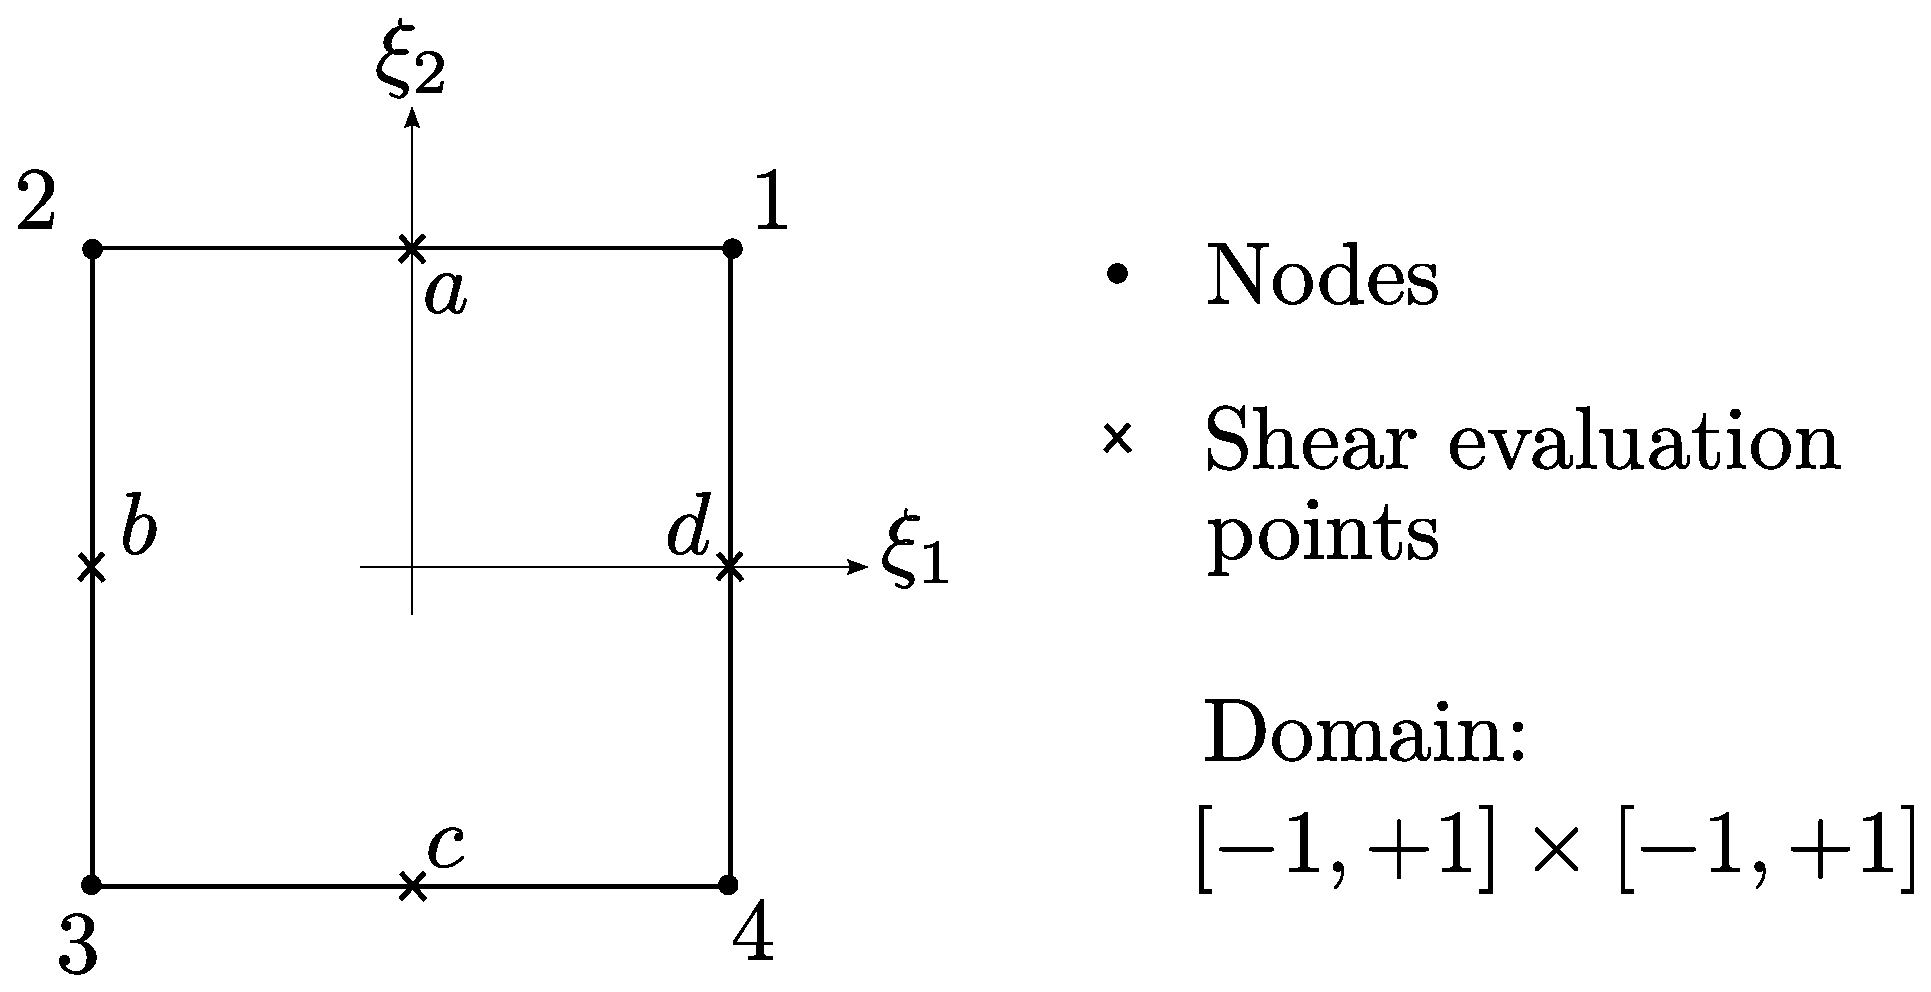
\includegraphics[width=.6\textwidth]{shellPic}
\caption{Shell: definitions}
\label{fig:EL:PLATE:SHELL4:sketch}
\end{figure}

Only linear elastic constitutive properties can be currently modeled.
They consist in a $12 \times 12$ matrix that expresses the force and moment
fluxes as functions of linear and angular strains according to
\begin{align}
	\cubr{\cvvect{
		n_{11} \\
		n_{12} \\
		n_{13} \\
		n_{21} \\
		n_{22} \\
		n_{23} \\
		m_{11} \\
		m_{12} \\
		m_{13} \\
		m_{21} \\
		m_{22} \\
		m_{23}
	}}
	&=
	\sqbr{D}
	\cubr{\cvvect{
		\varepsilon_{11} \\
		\varepsilon_{12} \\
		\varepsilon_{13} \\
		\varepsilon_{21} \\
		\varepsilon_{22} \\
		\varepsilon_{23} \\
		\kappa_{11} \\
		\kappa_{12} \\
		\kappa_{13} \\
		\kappa_{21} \\
		\kappa_{22} \\
		\kappa_{23}
	}}
\end{align}
When the \kw{isotropic} keyword is used, only two of the optional
sub-keywords \kw{E}, \kw{nu} and \kw{G} are required, as the remaining
parameter can be computed from the other two according to the relationship
\begin{align}
	\nt{G}
	&=
	\frac{\nt{E}}{2\plbr{1 + \nt{nu}}}
	.
\end{align}
If all are provided, they must be consistent.
The optional parameters \kw{as} and \kw{at} are not documented yet;
the default should be used.

\textbf{TODO: improve}



\subsection{Membrane4}
\label{sec:EL:PLATE:MEMBRANE4}

\emph{Authors: Marco Morandini and Tommaso Solcia}

The membrane4 element models a four-node membrane.
The syntax is
%\begin{verbatim}
\begin{Verbatim}[commandchars=\\\{\}]
    \bnt{elem_type} ::= \kw{membrane4eas} 

    \bnt{normal_arglist} ::=
        \bnt{node_1_label} , \bnt{node_2_label} , \bnt{node_3_label} , \bnt{node_4_label} ,
        \bnt{membrane_constitutive_law_data}

    \bnt{membrane_constitutive_law_data} ::=
        \{ [ \kw{matr} , ] \bnt{3x3_matrix}
            | \kw{sym} , \bnt{upper_triangular_3x3_matrix}
            | \kw{diag} , \bnt{diagonal_3x3_matrix}
            | \kw{isotropic} , \bnt{isotropic_data} \}
        [ , \kw{prestress} , (\ty{Vec3}) \bnt{prestress} ]

    \bnt{isotropic_data} ::=
        \{ \{ \kw{E} | \kw{Young modulus} \} , \bnt{E}
            | \{ \kw{nu} | \kw{Poisson modulus} \} , \bnt{nu}
            | \{ \kw{G} | \kw{shear modulus} \} , \bnt{G}
            | \kw{thickness} , \bnt{thickness} \}
        [ , ... ]
\end{Verbatim}
%\end{verbatim}
The name \kw{membrane4eas} stands for ``Enhanced Assumed Strain'' (EAS).
Nodes are numbered according to Figure~\ref{fig:EL:PLATE:SHELL4:sketch}.
Only linear elastic constitutive properties can be currently modeled.
They consist in a $3 \times 3$ matrix that expresses the force
fluxes as functions of linear strains according to
\begin{align}
	\cubr{\cvvect{
		n_{11} \\
		n_{22} \\
		n_{12}
	}}
	&=
	\sqbr{D}
	\cubr{\cvvect{
		\varepsilon_{11} \\
		\varepsilon_{22} \\
		\varepsilon_{12}
	}}
\end{align}
When the \kw{isotropic} keyword is used, only two of the optional
sub-keywords \kw{E}, \kw{nu} and \kw{G} are required, as the remaining
parameter can be computed from the other two according to the relationship
\begin{align}
	\nt{G}
	&=
	\frac{\nt{E}}{2\plbr{1 + \nt{nu}}}
	.
\end{align}
If all are provided, they must be consistent.





\section{User-Defined Elements}\label{sec:EL:BASE:USER_DEFINED}

\subsection{Loadable Element}\label{sec:EL:BASE:USER_DEFINED:LOADABLE}
Note: the \kw{loadable} element is deprecated in favor
of the \kw{user defined} element.

The \kw{loadable} element is a wrapper for a user-defined element that is
compiled in a separated module and linked run-time.
The module should provide a comprehensive set of functions according to 
a specified API; default functions are available if no special features
are required.
Implementation of modules can be very easy, but a deep knowledge of the
internals of the code is required when special tasks need to be performed. 
There are virtually no limits on what a loadable element can do.

The syntax is simply:
%\begin{verbatim}
\begin{Verbatim}[commandchars=\\\{\}]
    \bnt{elem_type} ::= \kw{loadable}

    \bnt{normal_arglist} ::= " \bnt{module_name} "
        [ , \kw{name} , " \bnt{calls} " ] 
        [ , \bnt{module_data} ]
\end{Verbatim}
%\end{verbatim}
where \nt{module\_name} is the name of the module file; as soon as the file
is checked and the binding of the structure with function bindings 
succeeded, a function called \texttt{read()} is invoked, passing it the input
stream.
This function is in charge of reading \nt{module\_data} following the
general syntax of the input file.

An alternative form is
%\begin{verbatim}
\begin{Verbatim}[commandchars=\\\{\}]
    \bnt{normal_arglist} ::= \kw{reference} , " \bnt{name} "
        [ , \bnt{module_data} ]
\end{Verbatim}
%\end{verbatim}
where \nt{name} is the name by which the loadable element recorded itself
when registered via the \kw{module load} directive, as described
in Section~\ref{sec:GENERAL:MODULE-LOAD}.
As a consequence, the following forms are equivalent:
\begin{verbatim}
    # direct runtime loading
    loadable: 1, "/some/module.so";
    # "/some/module.so" registers itself as "some_module"
    module load: "/some/module.so";
    loadable: 2, reference, "some_module";
    # works also as joint (might obsolete loadable elements)
    joint: 3, some_module;
\end{verbatim}

It is advisable that the function \texttt{read()} prints some help message
when the first field of \nt{module\_data} is the keyword \kw{help}.
All the helpers and the high-level structures are available, such as
drivers, constitutive laws, reference frames.
Refer to each module for a description (if available) of the features and of
the input/output format.
\nt{module\_name} should be a full path to the module function.
If the name starts with a slash ``/'', the full path name is used.
Otherwise the module is searched in the colon-separated list of directories 
contained in the environment variable \texttt{LD\_LIBRARY}, then among the
libraries listed in \texttt{/etc/ld.so.cache}, and finally in
\texttt{/usr/lib} and in \texttt{/lib} (see \texttt{dlopen(3)}).
At last, it is searched in the current directory, and the extension
\texttt{.so} is added if missing.
The string \nt{calls} represents the name of the structure that contains
the bindings to the functions.
The default is \texttt{calls}.

\noindent
Refer to \texttt{\$(BASE)/mbdyn/base/loadable.h} for a description of the
functions that are allowed.
An example module is given in directory
\begin{verbatim}
    $(BASE)/modules/module-template/
\end{verbatim}
which can be used as a starting point to build a custom module.
% An analogous C/FORTRAN style interface is being planned, at the cost of
% possibly losing some of the fancy C++ features made available by the code.
The \kw{loadable} element interface allows to link modules in different
languages, e.g.\ C or FORTRAN77; simply use \texttt{module-template}
as a guideline to providing callbacks to the \kw{loadable} element
interface and to collect required info from the main program
(e.g.\ node positions, equation indices and everything else that is
required for appropriate connection), then call the functions that
actually do the work in other languages from inside the callbacks.

\subsection{User-Defined Element}
The \kw{user defined} element is a much more streamlined form
of custom element definition than the \kw{loadable} element.
From the point of view of the syntax the differences are minimal;
however, from an implementation point of view, the \kw{user defined}
element is preferable.

The definition of a \kw{user defined} element requires two steps.
In the first step, a run-time loadable module is loaded using the 
\hyperref{\kw{module load} directive}{\kw{module load} directive (see Section~}{)}{sec:GENERAL:MODULE-LOAD}.
This registers a handler to the \kw{user defined} element type
along with a \nt{name} used to reference it.
In the second step, an instance of that \kw{user defined} element type
is created, referencing it by \nt{name}.

The syntax of the \kw{user defined} element is
%\begin{verbatim}
\begin{Verbatim}[commandchars=\\\{\}]
    \bnt{elem_type} ::= \kw{user defined}

    \bnt{normal_arglist} ::= \bnt{name} [ , \bnt{module_data} ]
\end{Verbatim}
%\end{verbatim}
As for the \kw{loadable} element, it is recommended that 
some useful output is given if the first \nt{module\_data}
is the keyword \kw{help}.

An example module is given in directory
\begin{verbatim}
    $(BASE)/modules/module-template2/
\end{verbatim}
which can be used as a starting point to build a custom module.

\paragraph{Example.} \
\begin{verbatim}
    module load: "libmodule-template2"

    user defined: 1000, template2, help;
\end{verbatim}



\subsection{General Discussion on Run-Time Loadable Modules}
In general, to call external functions from C++ one needs
to declare them as
\begin{verbatim}
    #include <sys/types.h>
    extern "C" {
        int a_C_function(int arg, double darg);
        int a_F77_subroutine(int32_t *iarg, double *darg);
    }
\end{verbatim}
The same applies to FORTRAN 77 functions; only, the naming convention
usually is compiler dependent; some compilers turn all the names to 
uppercase or lowercase (remember that FORTRAN 77 is case insensitive);
other compilers add underscores at the beginning or at the end of the
names.
Check what is the behavior of your compiler, by compiling a simple 
program with your favorite FORTRAN 77 compiler, then looking at it
with the utility \texttt{nm(1)}, which will show how the symbols are represented 
internally.

\noindent
For instance, the code
\begin{verbatim}
C This is a compiler test
      SUBROUTINE F77SUB(I, D)
      INTEGER*4 I
      REAL*8 D(*)

      D(I) = 0.0

      END
\end{verbatim}
when compiled with \texttt{g77(1)} on a GNU/Linux system, yields:
\begin{verbatim}
[masarati@mbdyn manual]$ g77 -c f77sub.f
[masarati@mbdyn manual]$ nm f77sub.o
00000000 T f77sub_
\end{verbatim}
That is, \texttt{g77(1)} lowercases all symbols, and adds a trailing 
underscore.
Macros to automatically detect and take care of this behavior 
are planned.


\noindent
To compile loadable modules, one needs to configure
the package as follows:
%\begin{verbatim}
\begin{Verbatim}[commandchars=\\\{\}]
    ./configure --with-module=\bnt{module_name}
\end{Verbatim}
%\end{verbatim}
where \nt{module\_name} is the name of the directory the module
is placed in with the \texttt{module-} part stripped; e.g.\ to compile
the tire module that resides in \texttt{\$(BASE)/modules/module-wheel2} 
one must type
\begin{verbatim}
    ./configure --with-module=wheel2
\end{verbatim}
Multiple modules can be compiled by typing the list of the names
separated by blanks.

\bigskip

\noindent
\fbox{\begin{minipage}{.96\textwidth}
The modules need to resolve some of the symbols that are in the
main executable; until a full working libtool support is implemented,
this must be done by hand.
The \texttt{g++(1)} compiler requires the switch `\texttt{-rdynamic}'
to be added to the loader's flags.
\end{minipage}}

\bigskip

For example,
%\begin{verbatim}
\begin{Verbatim}[commandchars=\\\{\}]
    ./configure --with-module=\bnt{module_name} LDFLAGS="-rdynamic" 
\end{Verbatim}
%\end{verbatim}





\section{Output Elements}
Output elements take care of inter-process communication.
These elements can use specific communication means,
depending on the type of simulation they are used for,
and can communicate specific types of data.

\subsection{Stream output}\label{sec:EL:OUTELEM:STREAM_OUTPUT}
This is a special element which takes care of sending output
to external processes by means of either \kw{local} or \kw{inet} sockets
during batch or real-time simulations.
This topic is under development, so expect frequent changes, and
please do not count too much on backward compatibility.

The syntax is:
%\begin{verbatim}
\begin{Verbatim}[commandchars=\\\{\}]
    \bnt{elem_type} ::= \kw{stream output}

    \bnt{arglist} ::=
        \kw{stream name} , " \bnt{stream_name} " ,
        \kw{create} , \{ \kw{yes} | \kw{no} \} ,
        [ \{ \kw{local} , " \bnt{socket_name} " , |
            [ \kw{port} , \bnt{port_number} , ]
            [ \kw{host} , " \bnt{host_name} " , ] \} ]
        [ \{ [ \kw{no} ] \kw{signal}
            | [ \kw{non} ] \kw{blocking}
            | [ \kw{no} ] \kw{send first}
            | [ \kw{do not} ] \kw{abort if broken} \} [ , ... ] , ]
        [ \kw{output every} , \bnt{steps} , ]
        [ \kw{echo} , \bnt{file_name}
            [ , \kw{precision} , \bnt{precision} ]
            [ , \kw{shift} , \bnt{shift} ] , ]
        \bnt{content}
\end{Verbatim}
%\end{verbatim}
The stream output allows MBDyn to send streamed outputs 
to remote processes during both batch and real-time simulations,
using sockets either in the \texttt{local} or in the \texttt{inet} namespace.
If the simulation is run in real-time using RTAI, RTAI mailboxes
are used instead.

\begin{itemize}
\item \nt{stream\_name} is the name of the RTAI mailbox where 
the output is written  (a unique string no more than six characters long);
it is basically ignored by the \kw{stream output} element
except when using RTAI;

\item the \kw{create} keyword determines whether the socket
must be created or looked-up as already existing on the system;
if \kw{create} is set to \kw{no}, MBDyn will retry for 60 seconds
and then give up;

\item \nt{socket\_name} is the path of the \kw{local} socket 
that is used to communicate between processes;

\item \nt{port\_number} is the port number to be used with a \texttt{inet} socket.
The default port number is 9011 (intentionally unassigned by IANA).
If no \nt{host\_name} is given, \kw{localhost} will be used;

\item \nt{host\_name} is the name or the IP of the remote host where
the mailbox resides; note that if this field is given, \kw{create} must
be set to \kw{no}.
The simulation will not start until the socket is created on the remote host;

\item the flag \kw{no signal} requests that no \texttt{SIGPIPE} be raised
when sending through a socket when the other end is broken
(by default, \texttt{SIGPIPE} is raised);

\item the flag \kw{non blocking} requests that operations on the socket
do not block (or block, in case of \kw{blocking}, the default);

\item the flag \kw{no send first} requests that no send occurs before
the first time step (by default, data is always sent);

\item the flag \kw{do not abort if broken} requests that the simulation
continues in case the connection breaks.
No further data send will occur for the duration of the simulation
(the default);

\item the field \kw{output every} requests output to occur
only every \nt{steps};

\item the field \kw{echo} causes the content that is sent to the peer
to be echoed on file \nt{file\_name}; the optional parameter \nt{precision}
determines the number of digits used in the output; the optional parameter
\nt{shift} is currently unused;

\item the field \nt{content} is detailed in the next section.
\end{itemize}
This element, when used with the \kw{motion} content type,
obsoletes the \kw{stream motion output} element
(see Section~\ref{sec:EL:OUTELEM:STREAM_MOTION_OUTPUT}).
When the simulation is executed in real-time using RTAI,
this element obsoletes the \kw{RTAI output} element
(see Section~\ref{sec:EL:OUTELEM:RTAI_out}).



\subsubsection{Streamed output}
Different types of data can be sent.
The most general form is called \kw{values}, consisting
in an arbitrary set of independent scalar channels.
A form specifically intended to communicate the motion
of a mechanical system is called \kw{motion}, consisting
in a subset of the kinematics of a set of structural nodes:
%\begin{verbatim}
\begin{Verbatim}[commandchars=\\\{\}]
    \bnt{content} ::= \{ \bnt{values} | \bnt{motion} \}

    \bnt{values} ::= [ \kw{values} , ]
        \bnt{channel_number} ,
            \bnt{value}
            [ , ... ]

    \bnt{value} ::=
        \{ [ \kw{nodedof} , ] (\ty{NodeDof}) \bnt{output_dof}
            | \kw{drive} , (\ty{DriveCaller}) \bnt{drive_data} \}

    \bnt{motion} ::= \kw{motion} ,
        [ \kw{output flags} ,
            \{ \kw{position}
                | \kw{orientation matrix}
                | \kw{orientation matrix transpose}
                | \kw{velocity}
                | \kw{angular velocity} \}
             [ , ... ] , ]
        \{ \kw{all} | \bnt{struct_node_label} [ , ... ] \}
\end{Verbatim}
%\end{verbatim}
where
\begin{itemize}
\item the (optional) keyword \kw{values} indicates that a set
of independent scalar channels is output by the element;

\item the number of channels \nt{channel\_number} that are written
determines how many \nt{value} entries must be read.
In case of \kw{nodedof} (the default, deprecated),
they must be valid scalar dof entries, which can be connected
in many ways to nodal degrees of freedom;
in case of \kw{drive}, they can be arbitrary functions,
including node or element private data;

\item the keyword \kw{motion} indicates that a subset of the kinematic
parameters of a set of structural nodes is output by the element.
As opposed to the \nt{values} case, which is intended for generic
interprocess communication output, this content type is intended to ease
and optimize the output of the motion of structural nodes,
to be used for on-line visualization purposes.
By default, only the position of the selected nodes is sent.
This is intended for interoperability with a development version
of EasyAnim which can read the motion info (the so-called ``van'' file)
from a stream.
The optional keyword \kw{output flags} allows to request the output
of specific node kinematics: the node position, orientation matrix
(either row- or column-major), the velocity and the angular velocity.
The default is equivalent to \texttt{\kw{output flags}, \kw{position}}.
\end{itemize}



\subsubsection{Non real-time simulation}
During non real-time simulations, streams operate in blocking mode.
The meaning of the parameters is:
\begin{itemize}
\item \nt{stream\_name} indicates the name the stream would be known as
by RTAI; it must be no more than 6 characters long, and mostly useless;

\item the instruction \kw{create} determines whether MBDyn will create
the socket, or try to connect to an existing one;

\item the keyword \kw{local} indicates that a socket 
in the local namespace will be used; if \kw{create} is set to \kw{yes},
the socket is created, otherwise it must exist.

\item either of the keywords \kw{port} or \kw{host} indicate that a socket
in the internet namespace will be used;

if \kw{create} is set to \kw{yes}, \nt{host\_name} indicates 
the host that is allowed to connect to the socket; it defaults 
to any host (\texttt{0.0.0.0}); if \kw{create} is set to \kw{no},
\nt{host\_name} indicates what host to connect to; the default 
is localhost (\texttt{127.0.0.1}); the default port is \kw{9011}
(intentionally unassigned by IANA);

\item the flag \kw{no signal} is honored;

\item the flag \kw{non blocking} is honored;

\item the flag \kw{no send first} is honored;

\item the flag \kw{do not abort if broken} is honored.
\end{itemize}
If no socket type is specified, i.e.\ none of the \kw{local}, \kw{port} 
and \kw{host} keywords are given, a socket is opened by default 
in the internet namespace with the default IP and port; the \kw{create}
keyword is mandatory.



\subsubsection{Real-time simulation}
During real-time simulations, streams wrap non-blocking RTAI mailboxes.
The meaning of the parameters is:
\begin{itemize}
\item the parameter \nt{stream\_name} indicates the name the stream
will be known as in RTAI's resource namespace; it must be exactly 6 characters long;

\item the instruction \kw{create} determines whether the mailbox will be
created or looked for by MBDyn;

\item the keyword \kw{local} is ignored;

\item the keyword \kw{host} indicates that a mailbox on a remote host 
will be used; it is useless when \kw{create} is set to \kw{yes}, because
RTAI does not provide the possibility to create remote resources;
if none is given, a local mailbox is assumed;

\item the keyword \kw{port} is ignored.

\item the flag \kw{no signal} is ignored;

\item the flag \kw{non blocking} is honored; however, blocking mailboxes
make little sense, and real-time synchronization using RTAI should not rely
on blocking mailboxes;

\item the flag \kw{no send first} is ignored (although it should be honored
when the mailbox is blocking);

\item the flag \kw{do not abort if broken} is ignored;
the program is always terminated if a mailbox is no longer available.
\end{itemize}





\subsection{RTAI output}\label{sec:EL:OUTELEM:RTAI_out}
This element is actually used only when the simulation is scheduled
using RTAI; otherwise, the corresponding \kw{stream output} element
is used (see Section~\ref{sec:EL:OUTELEM:STREAM_OUTPUT}).
As a consequence, its explicit use is discouraged and deprecated.
The \kw{stream output} element should be used instead.




\subsection{Stream motion output}\label{sec:EL:OUTELEM:STREAM_MOTION_OUTPUT}
This element type is obsoleted by the \kw{stream output} element
with the \kw{motion} content type
(see Section~\ref{sec:EL:OUTELEM:STREAM_MOTION_OUTPUT}).
The syntax is:
%\begin{verbatim}
\begin{Verbatim}[commandchars=\\\{\}]
    \bnt{elem_type} ::= \kw{stream motion output}

    \bnt{arglist} ::= 
        \kw{stream name} , " \bnt{stream_name} " ,
        \kw{create} , \{ \kw{yes} | \kw{no} \} ,
        [ \{ \kw{local} , " \bnt{socket_name} " ,
                | [ \kw{port} , \bnt{port_number} , ] [ \kw{host} , " \bnt{host_name} " , ] \} ]
        [ \{ [ \kw{no} ] \kw{signal}
                | [ \kw{non} ] \kw{blocking}
                | [ \kw{no} ] \kw{send first}
                | [ \kw{do not} ] \kw{abort if broken} \}
            [ , ... ] , ]
        \bnt{motion}
\end{Verbatim}
%\end{verbatim}
Its support may be discontinued in the future.


%\subsection{Structural output}
%\label{sec:EL:OUTELEM:STRUCTURAL_OUTPUT}
%TODO.



\section{Miscellaneous}
This section lists some extra cards that do not correspond to any
specific simulation entity, but rather alter the behavior 
of existing entries or cause special operations to be undertaken
during model input.



\subsection{Bind}\label{sec:EL:MISC:BIND}
The statement \kw{bind} does not really define an element.
It is rather used to instruct a
\htmlref{\kw{parameter node}}{sec:NODE:PARAMETER}
about which parameter of an element it is bound to.
The \kw{parameter node} must exist, and the element the node 
is being bound to, of type \nt{elem\_type} and label \nt{element\_label},
must have been already defined.
The complete syntax is:
%\begin{verbatim}
\begin{Verbatim}[commandchars=\\\{\}]
    \bnt{elem_type} ::= \kw{bind}

    \bnt{arglist} ::=
        \bnt{element_label} ,
        \bnt{element_type} ,
        \bnt{parameter_node_label} , 
        \bnt{bind_args}
\end{Verbatim}
%\end{verbatim}
where \nt{bind\_args} depend on the type of parameter node.

\subsubsection{Element}
When binding an element to an 
\htmlref{\kw{element}}{sec:NODE:PARAMETER:ELEMENT} parameter node,
each element makes a number of specific parameters available.
A detailed list is given for each element in the private data section.
In that case:
%\begin{verbatim}
\begin{Verbatim}[commandchars=\\\{\}]
    \bnt{bind_args} ::=
        \{ [ \kw{index} , ] \bnt{parameter_index}
            | \kw{string} , " \bnt{parameter_name} " \}
\end{Verbatim}
%\end{verbatim}
The value of \nt{parameter\_index} must be legal, i.e.\ between 1 and the
maximum number of parameters made available by the element.
The alternative form, using the keyword \kw{string} followed by
the \nt{parameter\_name}, allows more friendly definition of the binding.
The name of the parameter depends on the element whose property
is being bound.
A complete listing of the parameters that a parameter node 
can be bound to can be found in the `Private data' subsection
of each element's specification.

\paragraph{Example.} \
The parameter node \texttt{ANGLE} is bound to the rotation of a 
\hyperref{\kw{revolute hinge}}{\kw{revolute hinge} (see Section~}{)}{sec:EL:STRUCT:JOINT:REVOLUTE_HINGE}.
\begin{verbatim}
    # ... problem block

    begin: control data;
        structural nodes: 2;
        parameter nodes: 1;
        forces: 2;
        # ... other control data
    end: control data;

    set: integer NODE1 = 1000;
    set: integer NODE2 = 2000;
    set: integer ANGLE = 5000;
    set: integer REVOLUTE = 6000;

    begin: nodes;
        structural: NODE1, dynamic, null, eye, null, null;
        structural: NODE2, dynamic, null, eye, null, null;
        parameter: ANGLE, element;

        # ... other nodes
    end: nodes;

    begin: elements;
        joint: REVOLUTE, revolute hinge,
            NODE1,
                position, reference, node, null,
                orientation, reference, node, eye,
            NODE2,
                position, reference, node, null,
                orientation, reference, node, eye;
        bind: REVOLUTE, joint, ANGLE, string, "rx";
        couple: 1, NODE1, 0.,0.,1.,
            dof, ANGLE, parameter, 1, linear, 0.,1.;
        couple: 2, NODE2, 0.,0.,1.,
            element, REVOLUTE, joint, string, "rx", linear, 0.,1.;

        # ... other elements
    end: elements;
\end{verbatim}
Note that the same element data, i.e.\ the revolute hinge
relative rotation angle, is used to drive a couple in two different
ways; the latter, by means of the 
\hyperref{\kw{element} drive}{\kw{element} drive (see Section~}{)}{sec:DRIVE:ELEMENT}
is more direct, but the former, by means of the 
\hyperref{\kw{dof} drive}{\kw{dof} drive (see Section~}{)}{sec:DRIVE:DOF}
through the \kw{bind} mechanism has the additional effect of updating
the \kw{parameter} node, which can be used to connect
\htmlref{\kw{genel}}{sec:EL:GENEL} elements for special purposes.

\subsubsection{Beam strain gage}
When binding an element to a
\htmlref{\kw{beam strain gage}}{sec:NODE:PARAMETER:BEAM_STRAIN_GAGE}
parameter node, the \nt{element\_type} field must be \kw{beam}.
In that case:
%\begin{verbatim}
\begin{Verbatim}[commandchars=\\\{\}]
    \bnt{bind_args} ::= \bnt{beam_evaluation_point}
\end{Verbatim}
%\end{verbatim}
where \nt{beam\_evaluation\_point} is the evaluation point of the beam element
where the internal strain and curvatures must be evaluated.
It must be 1 for 2-node beams, while it can be either 1 or 2
for 3-node beams.

\paragraph{Example.} \
\begin{verbatim}
    # ... problem block

    begin: control data;
        parameter nodes: 1;
        beams: 1;
        # ... other control data
    end: control data;

    set: integer BEAM = 100;
    set: integer STRAIN = 200;

    begin: nodes;
        parameter: STRAIN, beam strain gage, 0.0, 0.1;
        # ... other nodes
    end: nodes;

    begin: elements;
        beam3: BEAM, ...; # beam data
        bind: BEAM, beam, STRAIN, 1;
        # ... other elements
    end: elements;
\end{verbatim}



\subsection{Driven Element}\label{sec:EL:BASE:DRIVEN}
The \kw{driven} type is not an element by itself. It is a wrapper that
masks another element and switches it on and off depending on the (boolean)
value of a drive. It can be used to emulate a variable topology model,
where some elements simply don't contribute to the residual
or to the Jacobian matrices when their drive has a certain value.
Since the drivers can be arbitrary functions of the time, 
or other parameters including the value of any degree of freedom, 
the driven elements can be ``driven'' in a very flexible way.
Every element can be driven, except those that can be instantiated once only.
The syntax for a driven element is:
%\begin{verbatim}
\begin{Verbatim}[commandchars=\\\{\}]
    \bnt{elem_type} ::= \kw{driven}

    \bnt{normal_arglist} ::= (\ty{DriveCaller}) \bnt{element_driver} ,
        [ \kw{hint} , " \bnt{hint} " [ , ... ] ] ,
        \bnt{driven_element}

    \bnt{driven_element} ::=
        \{ \kw{existing} : \bnt{driven_elem_type} , \bnt{driven_elem_label}
            | \bnt{element_card} \}
\end{Verbatim}
%\end{verbatim}
When the keyword \kw{existing} is used, an existing element 
of type \nt{driven\_elem\_type} and label \nt{driven\_elem\_label} is looked for, 
and it is wrapped by the driven element.
In this case, no new element is instantiated.
The label of the element must match that of the driving element given 
at the beginning.
For consistency with the syntax, and for more flexibility, 
even when wrapping an existing element the output flags can be set
at the end of the card.
This flag overrides the one set when the driven element was instantiated.

Otherwise, a regular element is read after the driving element's declaration;
it is then instantiated and wrapped by the \kw{driven} element wrapper.
Note that after the keyword \kw{existing} or after the driven element type,
a colon is used as a separator.
This is probably the only exception to the rule that the colon
can only follow a \nt{description} at the beginning of a card.
The label \nt{driven\_elem\_label} of the driven element must match that
of the driving element used at the beginning of the \kw{driven} card.

\paragraph{Example.} \
A pin constraint between two rigid bodies is released:
\begin{verbatim}
    set: integer BODY_1 = 1;
    set: integer BODY_2 = 2;
    # ...
    structural: BODY_1, dynamic,
        null, eye, null, null;
    structural: BODY_2, dynamic,
        null, eye, null, null;
    # ....
    body: BODY_1, BODY_1,
        1000., null, diag, 100.,100.,1.;
    body: BODY_2, BODY_2,
        10., null, diag, 1.e-1,1.e-1,1.e-3;
    # ...
    # this constraint will be released when Time = 10 s
    driven: 1, string, "Time<10.",
    joint: 1, spherical hinge,
        BODY_1,
            position, null,
        BODY_2,
            position, null;
\end{verbatim}

\paragraph{Example.} \
an
\hyperref{\kw{axial rotation}}{\kw{axial rotation} (see Section~}{)}{sec:EL:STRUCT:JOINT:AXIAL_ROTATION}
joint is replaced by a
\hyperref{\kw{revolute hinge}}{\kw{revolute hinge} (see Section~}{)}{sec:EL:STRUCT:JOINT:REVOLUTE_HINGE}
when the desired spin velocity, measured as the angular velocity
of the second node (assuming, for instance, that the first one is fixed),
is reached.
The value of an abstract node is used to input the angular velocity 
to the \kw{axial rotation} joint.
\begin{verbatim}
    set: integer BODY_1 = 1;
    set: integer BODY_2 = 2;
    set: integer CONTROL_OUTPUT = 3;
    # ...
    structural: BODY_1, static,
        null, eye, null, null;
    structural: BODY_2, dynamic,
        null, eye, null, null;
    abstract: CONTROL_OUTPUT;
    # ....
    driven: 1, node, BODY_2, structural, string, "Omega[3]",
        string, "Var < 100.",
    joint: 1, axial rotation,
        BODY_1,
            position, null,
            orientation, 1, 1.,0.,0., 3, 0.,0.,1.,
        BODY_2,
            position, null,
            orientation, 1, 1.,0.,0., 3, 0.,0.,1.,
        node, CONTROL_OUTPUT, abstract, string, "x",
            linear, 0.,1.;
    driven: 2, node, BODY_2, structural, string, "Omega[3]",
        string, "Var >= 100.",
    joint: 2, revolute hinge,
        BODY_1,
            position, null,
            orientation, 1, 1.,0.,0., 3, 0.,0.,1.,
        BODY_2,
            position, null,
            orientation, 1, 1.,0.,0., 3, 0.,0.,1.;
\end{verbatim}

\subsubsection{Hint}
The \kw{hint} feature consists in allowing the setup of elements
to be computed when they are activated rather than at startup.
For example, a joint that is activated after some simulation time
may need to compute its relative position and orientation
from the parameters of the simulation; a drive that controls
the evolution of the relative configuration of a joint may need
to infer its parameters from the current configuration
of the overall system; and so on.

Currently, only few elements, significantly joints, support 
and honor hints.
The typical syntax is given by a keywork followed by some optional
parameters within curly brackets.
For instance, the hint that instructs a joint to compute the offset
with respect to the second node when it is activated is
\begin{verbatim}
    driven: 10, string, "Time>1.", hint, "offset{2}",
    joint: 10, ...
\end{verbatim}
A similar form is used to instruct a joint to compute the relative
orientation with respect to node 1:
\begin{verbatim}
    driven: 20, string, "Time>1.", hint, "hinge{1}",
    joint: 20, ...
\end{verbatim}
A \kw{distance} joint may be fed a new drive by using:
\begin{verbatim}
    driven: 30, string, "Time>1.",
        hint, "drive{cosine,0.,pi/.1,-.9/2.,half,model::distance(1,2)}",
    joint: 30, distance, ... 
\end{verbatim}
A \kw{drive hinge} joint may be fed a new drive by using:
\begin{verbatim}
    driven: 40, string, "Time>1.",
        # note: the lines wrap for typographical reasons
        # in the actual file, the string has to be a single line
        hint, "drive3{model::xdistance(1,2),\
            model::ydistance(1,2), model::zdistance(1,2),\
            cosine,0.,pi/.1,-.9/2.,half,model::distance(1,2)}",
    joint: 30, drive hinge, ... 
\end{verbatim}

This feature will likely be extended to other elements
and generalized as much as possible.


\subsection{Inertia}\label{sec:EL:MISC:INERTIA}
This card causes the equivalent inertia properties of a subset
of elements to be generated.
%\begin{verbatim}
\begin{Verbatim}[commandchars=\\\{\}]
    \bnt{card} ::= \kw{inertia} : \bnt{label}
        [ , \kw{name} , " \bnt{inertia_name} " ]
        [ , \kw{position} , (\ty{Vec3}) \bnt{reference_position} ]
        [ , \kw{orientation} , (\ty{Mat3x3}) \bnt{reference_orientation} ]
        , \bnt{type_subset} [ , ... ]
        [ , \kw{output} , \{ \kw{no} | \kw{yes} | \kw{log} | \kw{both} \} ] ;

        \bnt{type_subset} ::= \bnt{type} , \{ \kw{all} | \bnt{label} [ , ... ] \}

        \bnt{type} ::= \{ \kw{body} | \kw{joint} | \kw{loadable} \}
\end{Verbatim}
%\end{verbatim}
where \kw{type} currently can be \kw{body}, \kw{joint} and \kw{loadable}, 
although more elements associated to inertia might participate in the future.
All elements whose labels are listed must exist, and duplicates
are detected and considered errors.
The keyword \kw{all} causes all the elements of type \nt{type} 
to be included in the list.

\noindent
The only effect of the \kw{inertia} statement is to log
each \kw{inertia} entry in the \texttt{.log} file in a self explanatory form,
referred both to the \kw{global} reference frame and to a reference frame
originating from \nt{reference\_position} and oriented 
as \nt{reference\_orientation}.
The optional parameter \kw{output} may be used to alter the default 
behavior:
\begin{itemize}
\item \kw{no} disables the output, making the \kw{inertia} 
statement essentially ineffective;
\item \kw{yes} enables output to standard output;
\item \kw{log} enables output to the \texttt{.log} file (the default);
\item \kw{both} enables output to both standard output and \texttt{.log} file.
\end{itemize}



\subsection{Output}\label{sec:EL:MISC:OUTPUT}
This card does not instantiate any \kw{element}; it rather enables
output of selected elements, and it is analogous to that of the
\hyperref{\kw{nodes}}{\kw{nodes} (see Section~}{)}{sec:NODE:MISC:OUTPUT}:
%\begin{verbatim}
\begin{Verbatim}[commandchars=\\\{\}]
    \bnt{card} ::= \kw{output} : \bnt{elem_type} , \bnt{elem_list} ;

    \bnt{elem_list} ::=
        \{ \bnt{elem_label}  [ , ... ]
            | \kw{range} , \bnt{elem_start_label} , \bnt{elem_end_label} \}
\end{Verbatim}
%\end{verbatim}
\nt{elem\_type} is a valid element type that can be read 
as card name in the \kw{elements} block.
In case the keyword \kw{range} is used, all existing elements comprised
between \nt{elem\_start\_label} and \nt{elem\_end\_label}
are set; missing ones are silently ignored.





